%%%%%%%%%%%%%%%%%%%%%
%   AMS packages    %
%%%%%%%%%%%%%%%%%%%%%

\documentclass[10 pt]{amsart}

\usepackage{amsmath}
\usepackage{amsxtra}
\usepackage{amscd}
\usepackage{amsthm}
\usepackage{amsfonts}
\usepackage{amssymb}
\usepackage{eucal}
\usepackage[all]{xy}
\usepackage{graphicx}
\usepackage{comment}
\usepackage{tikz}
\usepackage{tikz-cd}
\usepackage{latexsym,amsmath,amscd,amssymb,epsfig,verbatim}
\usepackage[margin=1in,letterpaper,portrait]{geometry}
\usepackage[colorinlistoftodos, textsize=tiny]{todonotes}
\usepackage{thmtools}
\usepackage{thm-restate}
\usetikzlibrary{matrix,calc, arrows,decorations.pathmorphing}

\addtolength{\oddsidemargin}{.5 in}
	\addtolength{\evensidemargin}{.4 in}
	\addtolength{\textwidth}{-1 in}

	\addtolength{\topmargin}{0 in}
	\addtolength{\textheight}{0 in}

\RequirePackage{color}
\definecolor{myred}{rgb}{0.75,0,0}
\definecolor{mygreen}{rgb}{0,0.5,0}
\definecolor{myblue}{rgb}{0,0,0.65}

\RequirePackage{ifpdf}
\ifpdf
  \IfFileExists{pdfsync.sty}{\RequirePackage{pdfsync}}{}
  \RequirePackage[pdftex,
   colorlinks = true,
   urlcolor = myblue, % \href{...}{...} external (URL)
   citecolor = mygreen, % \cite{...}
   linkcolor = myred, % \ref{...} and \pageref{...}
   pagebackref,
%   pdfpagemode=None,
   bookmarksopen=true]{hyperref}
\else
  \RequirePackage[hypertex]{hyperref}
\fi


\theoremstyle{plain}
  \newtheorem{thm}{Theorem}[section]
  \newtheorem{prop}[thm]{Proposition}
  \newtheorem{lem}[thm]{Lemma}
  \newtheorem{cor}[thm]{Corollary}
  \newtheorem{conjecture}[thm]{Conjecture}
\theoremstyle{definition}
  \newtheorem{defn}[thm]{Definition}
  \newtheorem{rem}[thm]{Remark}
  \newtheorem{eg}[thm]{Example}
  \newtheorem{ex}[thm]{Exercise}
  \newtheorem{question}[thm]{Question}
  \newtheorem{counterexample}[thm]{Counterexample}
  \newtheorem{convention}[thm]{Convention}
\theoremstyle{remark}
  \newtheorem{note}[thm]{Notation}
  \newtheorem*{note*}{Notation}

\numberwithin{equation}{section}

\newtheorem*{conjecture*}{Conjecture}
\newtheorem*{acknowledgement}{ACKNOWLEDGEMENT}

\newcommand\nc{\newcommand}
\nc\on{\operatorname}
\nc\renc{\renewcommand}
\newcommand\ssec{\subsection}
\newcommand\sssec{\subsubsection}
\newcommand\bO{{\mathbf O}}
\newcommand\CC{{\mathcal C}}
\newcommand\BN{{\mathbb N}}
\newcommand\BC{{\mathbb C}}
\newcommand\BF{{\mathbb F}}
\newcommand\BR{{\mathbb R}}
\newcommand\BQ{{\mathbb Q}}
\newcommand\BBZ{{\mathbb Z}}
\newcommand\uR{\underline{R}}
\newcommand\uZ{\underline{\BBZ}}
\newcommand\CF{{\mathcal E}}
\newcommand\uCF{\underline{{\mathcal E}}}
\newcommand\BZ{{\mathbb Z}}
\newcommand\BA{{\mathbb A}}
\newcommand\BP{{\mathbb P}}
\newcommand\fa{{\mathfrak a}}
\newcommand\fp{{\mathfrak p}}
\newcommand\fq{{\mathfrak q}}
\newcommand\fm{{\mathfrak m}}
\newcommand\pt{\mathrm{pt}}
\newcommand\rk{\operatorname{rk}}
\newcommand{\so}{\Rightarrow}
\newcommand{\upo}{\mathring}
\newcommand{\ra}{\rightarrow}
\renewcommand{\iff}{\Leftrightarrow}
\newcommand{\minus}{\backslash}
\renewcommand{\vec}[1]{\overrightarrow{#1}}
\renewcommand{\v}{\mathbf}
\newcommand{\gr}[1]{\langle {#1} \rangle}
\newcommand{\dstyle}{\displaystyle}
\renc{\mod}{\on{-mod}}
\newcommand{\id}{\mathrm{id}}
\nc{\ul}{\underline}



\newcommand\fbn{\mathcal H}
\newcommand \edgequot{\text{edge-quotient bijective }}

\def\Stab{\operatorname{Stab}}
\def\Fix{\operatorname{Fix}}
\newcommand\im{\text{Im}}

\makeatletter
\providecommand\@dotsep{5}
\def\listtodoname{List of Todos}
\def\listoftodos{\@starttoc{tdo}\listtodoname}
\makeatother

\title{Peckness of Edge Posets}
\author{David Hemminger, Aaron Landesman, Zijian Yao}

\address{David Hemminger, Duke University}
\email{david.hemminger@duke.edu}

\address{Aaron Landesman, Harvard University}
\email{aaronlandesman@gmail.com}

\address{Zijian Yao, Brown University}
\email{zijian$\_$yao@brown.edu}

\usepackage{amsmath}
\begin{document}



\begin{abstract}
For any graded poset $P,$ we define a new graded poset, $\mathcal E(P),$ whose elements are the edges in the Hasse diagram of P. For any group, $G,$ acting on the boolean algebra, $B_n,$ we conjecture that $\mathcal E(B_n/G)$ is Peck. We prove that the conjecture holds for ``common cover transitive'' actions. We give some infinite families of common cover transitive actions and show that the common cover transitive actions are closed under direct and semidirect products. We also prove that $\mathcal E(B_n/G)$ is unimodal and symmetric in the case that $G$ is the cyclic group or dihedral group.
\end{abstract}

\maketitle

\tableofcontents
\newpage

\listoftodos
\newpage

%%%%%%%%%%%%%%%%% Introduction %%%%%%%%%%%%%%%%%%
\section{Introduction}\label{sec:introduction}

Let $P$ be a finite graded poset of rank $n$.  In this paper we study the structure of the edges in the Hasse diagram of $P$.  To this end we define the \textit{edge poset construction} $\mathcal{E}$ as follows.

\begin{defn}
\label{defn:functor_of_edges}
For $P$ a finite graded poset, define its graded \textit{edge poset} $\mathcal{E}(P)$ as follows.  The elements of $\mathcal E(P)$ are pairs $(x,y)$ where $x,y\in P$, $x\le_P y$, and $\rk(y) = \rk(x) + 1$. Define the covering relation $\lessdot_{\mathcal E}$ on $\mathcal E(P)$ by $(x, y) \lessdot_{\mathcal E} (x^\prime, y^\prime)$ if $x\lessdot_P x^\prime$ and $y\lessdot_P y^\prime$, and define the relation $\le_{\mathcal E}$ on $\mathcal E(P)$ to be the transitive closure of $\lessdot_{\mathcal E}$.  Finally define a rank function on $\mathcal{E}(P)$ by $\rk_{\mathcal{E}(P)}(x,y) = \rk_P(x)$.
\end{defn}
%Let $Q$ be a finite graded poset of rank $n$.  Given a morphism $f\colon P\rightarrow Q$, define $\mathcal E(f)\colon \mathcal E(P)\rightarrow \mathcal E(Q)$ by $\mathcal E(f)(x,y) = (f(x), f(y))$.


Note that since an edge in the Hasse diagram of $P$ can be identified with a pair $(x,y)\in P\times P$ such that $x\lessdot y$, the edges are in bijection with elements $(x,y)\in \mathcal E(P)$ via this identification.  We will show that $\mathcal{E}(P)$ is a well-defined graded poset in Section \ref{sec:functor_of_edges}. 

\begin{eg}
We give an example of an edge poset in Figure \ref{fig:EP_definition_example}.  Note that it is important we declare the relation $\leq_\mathcal E$ to be the transitive closure of $\lessdot_{\mathcal E}$.  If instead we defined a relation $\le_{\mathcal{E^\prime}}$ on $\mathcal{E}(P)$ by $(x, y) \leq (a, b)$ if $x \leq a, y \leq b$, then $\mathcal{E}(P)$ would not necessarily be a graded poset.  In Figure \ref{fig:EP_definition_example} we give an example of a poset $P$ for which $\mathcal{E}(P)$ is not graded with the relation $\le_{\mathcal{E^\prime}}$.  In the figure it is clear that $\mathcal E(P)$ is a graded poset, with $rk(x,y) = rk(x),$ but the Hasse diagram on the right represents a poset which does not have a grading.

%On the left hand side is the Hasse diagram of a poset $P$ in the middle is the poset $\mathcal E(P)$ and on the right hand side is the poset obtained from the relation 


\begin{figure}[h!]
\begin{center}
\[
\raisebox{1mm}{
\begin{tikzpicture}[scale=.7] at (0,0)
  \node (0) at (0,0) {$0$};
  \node (1) at (-1,2) {$1$};
  \node (2) at (1,2) {$2$};
  \node (3) at (0,4) {$3$};
  \node (4) at (2,4) {$4$};
  \node (5) at (0,6) {$5$};
  \node (6) at (2,6) {$6$};
  \node (7) at (1,8) {$7$};
  \draw (0)--(1);
  \draw (0)--(2);
  \draw (1)--(3);
  \draw (2)--(3);
  \draw (2)--(4);
  \draw (3)--(5);
  \draw (4)--(6);
  \draw (5)--(7);
  \draw (6)--(7);
  \node (8) at (0,-2) {$P$};
\end{tikzpicture}
} \qquad
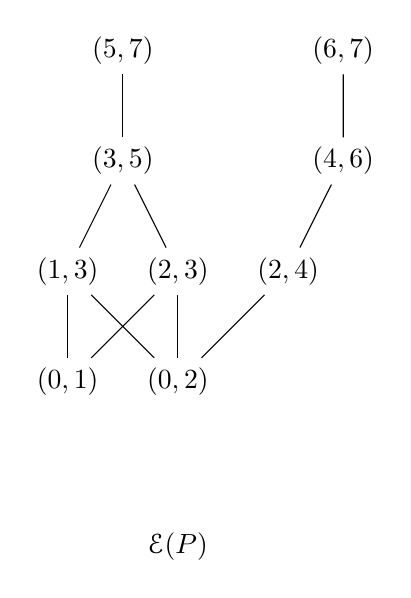
\begin{tikzpicture}[scale = .7]
  \node (0) at (0,1) {$(0,1)$};
  \node (1) at (2,1) {$(0,2)$};
  \node (2) at (0,3) {$(1,3)$};
  \node (3) at (2,3) {$(2,3)$};
  \node (4) at (4,3) {$(2,4)$};
  \node (5) at (1,5) {$(3,5)$};
  \node (6) at (5,5) {$(4,6)$};
  \node (7) at (1,7) {$(5,7)$};
  \node (8) at (5,7) {$(6,7)$};
  \draw (0)--(2);
  \draw (1)--(3);
  \draw (1)--(4);
  \draw (2)--(5);
  \draw (3)--(5);
  \draw (4)--(6);
  \draw (5)--(7);
  \draw (6)--(8);
  \draw (0)--(3);
  \draw (1)--(2);
  \node (9) at (2,-2) {$\mathcal E(P)$};
\end{tikzpicture}
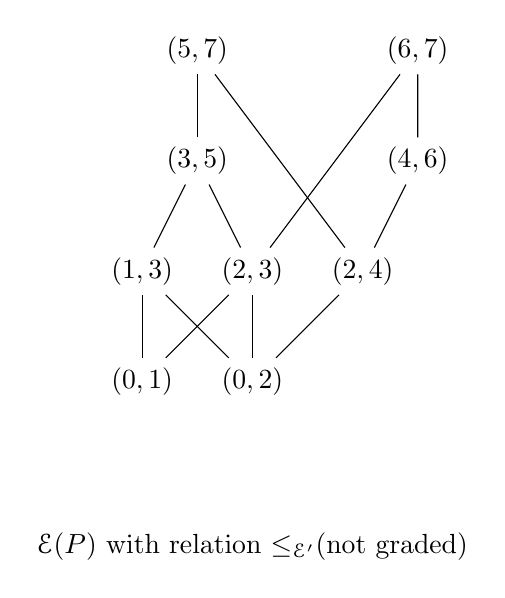
\begin{tikzpicture}[scale = .7]
  \node (0) at (0,1) {$(0,1)$};
  \node (1) at (2,1) {$(0,2)$};
  \node (2) at (0,3) {$(1,3)$};
  \node (3) at (2,3) {$(2,3)$};
  \node (4) at (4,3) {$(2,4)$};
  \node (5) at (1,5) {$(3,5)$};
  \node (6) at (5,5) {$(4,6)$};
  \node (7) at (1,7) {$(5,7)$};
  \node (8) at (5,7) {$(6,7)$};
  \draw (0)--(2);
  \draw (1)--(3);
  \draw (1)--(4);
  \draw (2)--(5);
  \draw (3)--(5);
  \draw (4)--(6);
  \draw (5)--(7);
  \draw (6)--(8);
  \draw (4)--(7);
  \draw (3)--(8);
  \draw (0)--(3);
  \draw (1)--(2);
  \node (9) at (2,-2) {$\mathcal E(P)$ with relation $\le_{\mathcal{E^\prime}}$(not graded)};
\end{tikzpicture}
\]



\iffalse
\newline
\begin{tikzpicture}[scale=.7]
  \node (one) at (90:2cm) {$6$};
  \node (b) at (150:2cm) {$4$};
  \node (a) at (210:2cm) {$2$};
  \node (zero) at (270:2cm) {$1$};
  \node (c) at (330:2cm) {$3$};
  \node (d) at (30:2cm) {$5$};
  \draw (zero) -- (a) -- (b) -- (one) -- (d) -- (c) -- (zero);
\end{tikzpicture}
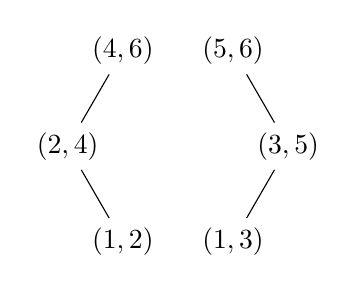
\begin{tikzpicture}[scale=.7]
  \node (one) at (60:2cm) {$(5, 6)$};
  \node (b) at (120:2cm) {$(4, 6)$};
  \node (a) at (180:2cm) {$(2, 4)$};
  \node (zero) at (240:2cm) {$(1, 2)$};
  \node (c) at (300:2cm) {$(1,3)$};
  \node (d) at (0:2cm) {$(3, 5)$};
  \draw (zero) -- (a) -- (b);
  \draw (c)--(d)--(one);
\end{tikzpicture}
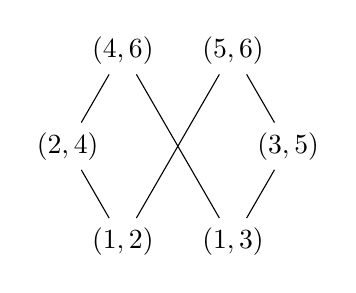
\begin{tikzpicture}[scale=.7]
  \node (one) at (60:2cm) {$(5, 6)$};
  \node (b) at (120:2cm) {$(4, 6)$};
  \node (a) at (180:2cm) {$(2, 4)$};
  \node (zero) at (240:2cm) {$(1, 2)$};
  \node (c) at (300:2cm) {$(1, 3)$};
  \node (d) at (0:2cm) {$(3, 5)$};
  \draw (zero) -- (a) -- (b) -- (c)--(d)--(one) -- (zero);
\end{tikzpicture}
\fi
\caption{\label{fig:EP_definition_example}The definition of $\mathcal E$}
\end{center}
\end{figure}
\end{eg}


We observe that when $P$ has a nice structure, $\mathcal E(P)$ commonly has a nice structure as well.  In particular we examine the \textit{boolean algebra of rank $n$}, denoted $B_n$, which is defined to be the poset whose elements are subsets of $\{1,\ldots,n\}$ with the relation given by containment, i.e. for all $x,y\in B_n$, $x\le y$ if $x$ is a subset of $y$.

Throughout the paper we say a group $G$ acts on $P$ if it acts on the elements of $P$ and that action is order-preserving and rank-preserving, i.e. for all $g \in G$ we have $x \leq y \iff gx \leq gy$ and $\rk(gx) = rk(x)$.  By Theorem \ref{thm:quotients_of_unitary_peck_posets} and the fact that $B_n$ is unitary peck, if $G$ is any action on $B_n,$ then $B_n/G$ is Peck.  We conjecture the following.

\begin{conjecture}\label{conj:F_of_BnG_Peck}
If $G \subset Aut(B_n),$ then $\mathcal E(B_n/G)$ is Peck.
\end{conjecture}

We prove this conjecture holds whenever the group action of $G$ on $B_n$ has the following property.

\begin{defn}
\label{defn:cover_transitive}
A group action of $G$ on $P$ is \textit{common cover transitive} (CCT) if whenever $x,y,z\in P$ such that $x\lessdot z$, $y\lessdot z$, and $y\in Gx$ there exists some $g\in Stab(z)$ such that $g\cdot x = y.$
\end{defn}

\begin{restatable}{thm}{cctpeck}
\label{thm:cover_transitive_implies_Peck}
If a group action of $G$ on $B_n$ is CCT, then $\mathcal E(B_n/G)$ is Peck.
\end{restatable}

A large number of group actions on $B_n$ have the CCT property.  We first prove that some basic group actions on $B_n$ are CCT.  Throughout the paper we let a subgroup $G\subseteq S_n$ act on $B_n$ by letting it act on the elements within subsets of $[n]:= \{1,\ldots, n\}$, i.e. $g\cdot x = \{g\cdot i\colon i\in x\}$  for all $g\in G$, $x\in B_n$.  We also embed the dihedral group $D_{2n}$ into $S_n$ by letting it act on the vertices of an $n$-gon.

\begin{restatable}{prop}{building}
\label{prop:cover_transitive_building_blocks}
Let $p$ be prime.  The following actions are CCT.

\begin{enumerate}
\item The action of $S_n$ on $B_n$.
\item The action of $D_{2p}$ on $B_p$.
\item The action of $D_{4p}$ on $B_{2p}$.
\end{enumerate}
\end{restatable}

We then show that cover transitivity is preserved under semidirect products, allowing us to describe several large families of CCT actions in Section \ref{ssec:CCT_examples}.

\begin{restatable}{prop}{semidirect}
\label{prop:semidirect_product_preservation}
Let $G\subseteq \operatorname{Aut}(P)$, $H\triangleleft G$, $K\subset G$ such that $G = H\rtimes K$.  Suppose that the action of $H$ is on $P$ is CCT and the action of $K$ on $P/H$ is CCT. Then the action of $G$ on $P$ is CCT.
\end{restatable}

The paper is organized as follows. In Section \ref{sec:background} we cover the necessary background for posets and Peck posets.  In Section \ref{sec:functor_of_edges} we show that $\mathcal E$ is well-defined and prove Theorem \ref{thm:cover_transitive_implies_Peck} along with various other nice properties of $\mathcal E$. Section \ref{sec:cover_transitive} contains the proofs of Propositions \ref{prop:cover_transitive_building_blocks} and \ref{prop:semidirect_product_preservation} as well as some examples of families of group actions shown to be CCT by these propositions. In Section \ref{sec:wreath_product}, we demonstrate formulas for certain generalizations of the edge poset applied to the quotient of $B_{m \cdot l}/S_m \wr S_l$ and obtain as a corollary \cite[Theorem 1.1]{pak}. Then, in Section \ref{sec:polya}, we use Polya theory to obtain and investigate formulas for the ranks of the generalized edge posets of $B_n/G.$ In Section \ref{sec:unimodal} we prove that $\mathcal E(B_n/G)$ is rank-unimodal for certain group actions that are not CCT. Then, in Section \ref{sec:unitary_peck_f}, we give a computational proof that $\mathcal E(B_n)$ is unitary Peck. Finally, in Section \ref{sec:additional_stuff}, we describe additional aspects of this problem we examined, an approach that didn't quite pan out, and further questions.



%%%%%%%%%%%%%%%%%  Background   %%%%%%%%%%%%%%%%%%
\section{Background}\label{sec:background}
In this section we review morphisms of graded posets, Peck posets, and a useful theorem about quotients of Posets. 

Throughout the paper we write $x\le_P y$ to denote that $x$ is less than or equal to $y$ under the relation defined on the poset $P$. When the poset is clear we will omit the $P$ and simply write $x\le y$.

A poset $P$ a {\it graded} poset if it there exists a rank function $\rk:P \rightarrow \BZ_{\geq 0}$ satisfying the following conditions.
\begin{enumerate}
	\item If $x\in P_i$ and $x\lessdot y$, then $rk(x) + 1 = rk(y),$
	\item If $x < y$ then $\rk(x) < rk(y)$ 
\end{enumerate}
Then, define the $i$th rank of $P$ to be  $P_i = \{x \in P\colon\rk(x) = i\}.$ Additionally, if for all $x\in P,0 \leq \rk(x) \leq n,$ and there exists $x,y$ with $\rk(x) = 0, rk(y) = n,$ we say $P$ is a graded poset of {\it rank $n$}.

Denote the category of finite graded posets by $\mathcal{P}$, and let $P,Q$ be finite graded posets of rank $n$.  A map $f\colon P\rightarrow Q$ is a \textit{morphism} from $P$ to $Q$ if it is rank-preserving and order preserving, i.e. for all $x,y\in P$, $x\le_P y \Rightarrow f(x)\le_Q f(y)$ and $\rk(x) = \rk(f(x))$.  We say that $f$ is \textit{injective/surjective/bijective} if it is an injection/surjection/bijection from $P$ to $Q$ as sets.

\begin{rem}\label{rem:bijective_morphism_not_isomorphism}
Note that we do not require the implication $f(x)\le_Q f(y) \Rightarrow x\le_P y$ in order for $f$ to be a morphism.  In particular this means a bijective morphism $f$ need not be an isomorphism, since it will not necessarily have a two-sided inverse.  
%There is an important distinction here between bijection and isomorphism. Another way to describe a bijection is that it is an embedding $f:P\rightarrow Q$ which is a bijection on the sets of vertices of $P,Q$. But, an isomorphism also defines a bijection between the edges of the two posets as well.
\end{rem}

Write $p_i = |P_i|$.  If we have

$$p_0\le p_1\le \ldots \le p_k \ge p_{k+1} \ge\ldots \ge p_n$$

\noindent for some $0\le k\le n$, then $P$ is \textit{rank-unimodal}, and if $p_i = p_{n-i}$ for all $1\le i\le n,$ then $P$ is \textit{rank-symmetric}.  An \textit{antichain} in $P$ is a set of elements in $P$ that are pairwise incomparable.  If no antichain in $P$ is larger than the largest rank of $P$, then $P$ is \textit{Sperner}.  More generally, $P$ is \textit{$k$-Sperner} if no union of $k$ antichains in $P$ is larger than the union of the largest $k$ ranks of $P$, and $P$ is \textit{strongly Sperner} if it is $k$-Sperner for all $1\le k\le n$.  We then make the following definition.

\begin{defn}
$P$ is \textit{Peck} if $P$ is rank-symmetric, rank-unimodal, and strongly Sperner.
\end{defn}


Let $V(P)$ and $V(P_i)$ be the complex vector spaces with bases $\{x :x\in P\}$ and $\{x :x\in P_i\}$ respectively.  Note that we will frequently abuse notation and write $P$ and $P_i$ for $V(P)$ and $V(P_i)$ when our meaning is clear.  In determining whether $P$ is Peck, it is often useful to consider certain linear transformations on $V(P)$.

\begin{defn}
\label{defn:lefschetz}
A map $U\colon V(P)\rightarrow V(P)$ is an \textit{order-raising operator} if $U(V(P_n)) = 0$ and for all $0\le i\le n-1$, $x\in P_i$ we have

$$U(x) = \sum_{y\gtrdot x} c_{x,y}y$$

\noindent for some constants $c_{x,y}\in \mathbb{C}$.  We say that $U$ is the \textit{Lefschetz map} if all $c_{x,y}$ on the right hand side are equal to 1.
\end{defn}

\noindent We then have the following well-known characterization of Peck posets.

\begin{lem}[\cite{weyl_groups_stanley}, Lemma 1.1]\label{lem:Peck_poset_characterization}
$P$ is Peck if and only if there exists an order-raising operator $U$ such that for all $0\le i < \frac{n}{2}$, the map $U^{n-2i}\colon V(P_i)\rightarrow V(P_{n-i})$ is an isomorphism.
\end{lem}

\begin{defn}
If the Lefschetz map satisfies the condition for $U$ in Lemma \ref{lem:Peck_poset_characterization}, then $P$ is \textit{unitary Peck}.
\end{defn}


We say that a group $G$ acts on $P$ if the action defines and embedding $G\hookrightarrow \operatorname{Aut}(P)$, and define the \textit{quotient poset} $P/G$ to be the poset whose elements are the orbits of $G$, with the relation $\mathcal{O}\le \mathcal{O}^\prime$ if there exist $x\in \mathcal{O}$, $x^\prime\in \mathcal{O}^\prime$ such that $x\le x^\prime$.  We will use the following result later in the paper.

\begin{thm}[\cite{quotients_stanley}, Theorem 1]
\label{thm:quotients_of_unitary_peck_posets}
If $P$ is unitary Peck and $G\subseteq\operatorname{Aut}(P)$, then $P/G$ is Peck.
\end{thm}


%%%%%%%%%%%%%%%%% The Edge Functor  %%%%%%%%%%%%%%%%%%

\section{The Edge Poset Construction}
\label{sec:functor_of_edges}

In Section \ref{ssec:definition_and_basic_properties} we show that $\mathcal E$ as described in Definition \ref{defn:functor_of_edges} is well-defined and prove some useful properties of $\mathcal E$.  Section \ref{ssec:proof_of_cover_transitive_implies_Peck} is devoted to the proof of Theorem \ref{thm:cover_transitive_implies_Peck}.  In Section \ref{ssec:E_generalization} we discuss a possible generalization for $\mathcal{E}$.

\ssec{Definition and Basic Properties}\label{ssec:definition_and_basic_properties}
First we show that $\mathcal{E}$ is well-defined in Lemmas \ref{lem:f_partial_order} and \ref{lem:FP_graded_poset}.  After showing that $\mathcal E$ is well-defined we then define a natural $G$ action on $\mathcal E(P)$ and define a surjection $\mathcal E(P)/G\rightarrow \mathcal E(P/G)$ that will be important for the proof of Theorem \ref{thm:cover_transitive_implies_Peck}. Finally, we prove the simple result that $\mathcal E$ sends self-dual posets to self-dual posets.

\begin{note*}
When the poset $P$ is clear, we shall simply use $\leq_{\mathcal E},\lessdot_{\mathcal E}$ to refer to $\leq_{\mathcal E(P)},\lessdot_{\mathcal E(P)}.$ Similarly, in Subsection ~\ref{ssec:proof_of_cover_transitive_implies_Peck}, we define an object $\mathcal H(B_n),$ and shall use $\leq_{\mathcal H},\lessdot_{\mathcal H}$ in place of $\leq_{\mathcal H(P)},\lessdot_{\mathcal H(P)}.$
\end{note*}

\begin{lem}\label{lem:f_partial_order}
The relation $\le_{\mathcal E}$ defines a partial order on $\mathcal E(P)$.
\end{lem}

\begin{proof}
We have that $(x, y)\le_{\mathcal E} (x, y)$ and that $\le_{\mathcal E}$ is transitive by definition.  It remains to be shown that $\le_{\mathcal E}$ is antisymmetric.  Suppose $(x, y)\le_{\mathcal E} (x^\prime, y^\prime)$ and $(x^\prime, y^\prime)\le_{\mathcal E} (x, y)$.  Then $x\le_P x^\prime \le_P x$ and $y\le_P y^\prime \le_P y$, so $x = x^\prime$ and $y=y^\prime$ by antisymmetry of $\le_P$, hence $(x, y) = (x^\prime, y^\prime)$.
\end{proof}

\begin{lem}\label{lem:FP_graded_poset}
For $P$ a graded poset, the object $\mathcal E(P)$ is a graded poset.
\end{lem}

\begin{proof}
To show $\mathcal E(P)$ is graded, we must show that $(x, y) \lessdot_{\mathcal E} (x^\prime, y^\prime) \implies \rk(x, y)+1 = \rk(x^\prime , y^\prime)$.  This fact follows immediately from the definition of $\lessdot_{\mathcal E}$ and the definition $\rk_{\mathcal E}(x, y) = \rk_P(x)$.
\end{proof}

%First, if $x\otimes y <_{\mathcal E} a \otimes b$ then by definition of $<_{\mathcal E}$, we must have $x < x^\prime,$ and hence 
%$$rk_{\mathcal E}(x\otimes y) = rk_P(x)<rk_P(x^\prime) = rk_{\mathcal E}(x^\prime\otimes y^\prime).$$
%Second, if $x\otimes y \lessdot_{\mathcal H} x^\prime \otimes y^\prime$ then $x \lessdot_P x^\prime,$ so $rk(x)+1 = rk(x^\prime)$ and then $$rk_{\mathcal E}(x\otimes y)+1 = rk_P(x) +1=rk_P(x^\prime)= rk_{\mathcal E}(x^\prime\otimes y^\prime).$$



In order to define a group action, we will define more generally a way for morphisms of posets to induce morphisms of their edge posets.

\begin{lem}\label{lem:Ff_poset_morphism}
Let $f\colon P\rightarrow Q$ be a morphism of finite graded posets, and define a map $\mathcal E(f)\colon \mathcal E(P)\rightarrow \mathcal E(Q)$ by $\mathcal{E}(f)(x,y) = (f(x),f(y))$ for all $(x,y)\in \mathcal{E}(P)$.  Then

\begin{enumerate}
\item $\mathcal{E}(f)$ is a morphism of finite graded posets
\item $\mathcal{E}(\id_P) = \id_{\mathcal{E}(P)}$
\item If $g\colon Q\rightarrow R$ is a morphism of finite graded posets, then $\mathcal E(g\circ f) = \mathcal E(g)\circ\mathcal E(f)$.
\end{enumerate}
\end{lem}

\begin{proof}

\vskip.1in
\noindent
{\sf Part (1)}
First, $\mathcal E(f)$ is rank-preserving, since for all $(x, y)\in \mathcal E(P)$ we have 
$$\rk_{\mathcal E}(x, y) = \rk_P(x) = \rk_P(f(x)) = \rk_{\mathcal E}(\mathcal E(f)(x, y)).$$
Suppose $(x, y)\le_{\mathcal E} (x^\prime, y^\prime)$.  Then $x\le_P x^\prime$, $y\le_P y^\prime$, and since $f$ is order-preserving, it follows that $f(x)\le_P f(x^\prime)$, $f(y)\le_P f(y^\prime)$. Hence $\mathcal E(f)(x,y) \le_{\mathcal E} \mathcal E(f)(x^\prime , y^\prime)$.  Thus $\mathcal E(f)$ is order-preserving and hence a morphism of finite ordered posets.

\vskip.1in
\noindent
{\sf Part (2)} This is trivial.

\vskip.1in
\noindent
{\sf Part (3)} For all $(x, y)\in \mathcal E(P)$ we have 
$$\mathcal E(g\circ f)(x, y) = (g(f(x)), g(f(y))) = \left(\mathcal E(g)\circ\mathcal E(f)\right)(x, y).$$
\end{proof}

%\begin{prop}\label{prop:F_well_defined}
%The map $\mathcal E(P)$ is an endofunctor on the category of finite graded posets $\mathcal{P}$.
%\end{prop}
%
%\begin{proof}
%By Lemmas \ref{lem:f_partial_order}, \ref{lem:FP_graded_poset}, and \ref{lem:Ff_poset_morphism} we have that $\mathcal E$ takes objects in $\mathcal{P}$ to objects in $\mathcal{P}$ and morphisms of $\mathcal{P}$ to morphisms of $\mathcal{P}$.  Furthermore it is clear that $\mathcal E(\id_P) = \id_{\mathcal E(P)}$, so it remains to be shown that for finite graded posets $P, Q,$ and $R$ with morphisms $f\colon P\rightarrow Q$ and $g\colon Q\rightarrow R$ that $\mathcal E(g\circ f) = \mathcal E(g)\circ\mathcal E(f)$.  This is clear, however, as for all $(x, y)\in \mathcal E(P)$ we have $\mathcal E(g\circ f)(x, y) = (g(f(x)), g(f(y))) = \left(\mathcal E(g)\circ\mathcal E(f)\right)(x, y)$.
%\end{proof}

\begin{rem}
By Lemma \ref{lem:Ff_poset_morphism}, the edge poset construction $\mathcal{E}$ defines an endofunctor on the category finite graded posets with rank-preserving morphisms.
\end{rem}



Given a group action of $G$ on $P$, we can now easily define a natural group action of $G$ on $\mathcal E(P)$ using Lemma \ref{lem:Ff_poset_morphism}.  For all $g\in G$ we have that multiplication by $g$ is an automorphism of $P$, so it follows that $\mathcal E(g)$ is an automorphism of $\mathcal E(P)$ and furthermore that this gives a well-defined group action by Lemma \ref{lem:Ff_poset_morphism}.

\begin{defn}\label{note:G_action_on_FP}
Given a $G$-action on $P$, define a $G$-action on $\mathcal E(P)$ by $g\cdot (x,y) = \mathcal{E}(g)(x,y) = (gx,gy)$.
\end{defn}

We then have a well-defined quotient poset $\mathcal E(P)/G$.  It is natural to ask whether the operation of quotienting out by $G$ commutes with $\mathcal E$, that is, whether $\mathcal E(P/G) \cong \mathcal E(P)/G$.  Unfortunately the two posets are rarely isomorphic, but there is always a surjection $\mathcal E(P)/G\rightarrow \mathcal E(P/G)$, and this surjection is also an injection precisely when the $G$-action on $P$ is CCT.


\begin{prop}\label{prop:surjection_between_F_quotients}
%For any group $G$ acting on $P$ and $0\le i\le \rk(P)$, we have $|\mathcal E(P/G)|_i \le |\mathcal E(P)/G|_i$.
The map $q\colon \mathcal E(P)/G\rightarrow \mathcal E(P/G)$ defined by $q(G(x, y)) = (Gx,Gy)$ is a surjective morphism.
\end{prop}

\begin{proof}
%Let $Gx\otimes Gy\in \mathcal E(P/G)$.  Since the orbits between $Gx$ and $Gy$ form a boolean algebra of size $r$, it is possible to pick a set of representatives from the orbits in $Gx\otimes Gy$ such that the representatives form a boolean subalgebra $x\otimes y$ of size $r$ in $P$.  Then $x\otimes y\in \mathcal E(P)$ and the orbit $G(x\otimes y)$ is in $\mathcal E(P)/G$.  Furthermore, if $Gy^\prime\otimes Gx^\prime \ne Gy\otimes Gx$, then any boolean subalgebra $x^\prime\otimes y^\prime$ given by representatives from orbits lying between $Gx^\prime$ and $Gy^\prime$ will not be an element of $G(x\otimes y)$, since $(Gx,Gy)\ne (Gx^\prime,Gy^\prime)$.  Thus a choice of representatives from each boolean subalgebra of size $r$ in $\mathcal E(P/G)$ gives a rank-preserving injection $\mathcal E(P/G)\rightarrow \mathcal E(P)/G$ and hence $|\mathcal E(P/G)|_i \le |\mathcal E(P)/G|_i$.

%Now consider the case when $r = 1$.  A boolean subalgebra of size 1 simply corresponds to an edge between adjacent ranks defined by a covering relation $x\lessdot y$ for some $x,y\in P$.  Then for every edge $x\otimes y\in \mathcal E(P)$, the orbit $Gx\otimes Gy$ is an element of $\mathcal E(P/G)$, so we get a map $q\colon \mathcal E(P)/G \rightarrow \mathcal E(P/G)$ by defining $q(G(x\otimes y)) = Gx\otimes Gy$. 


Note that $q$ is well defined because if $(x^\prime, y^\prime) = g(x, y) = (g\cdot x, g\cdot y)$ for some $g\in G$, then $x^\prime\in Gx$ and $y^\prime\in Gy$.  Clearly $q$ is rank-preserving and surjective, so it suffices to show that $q$ is order-preserving.  Suppose that $G(x, y) \le G(w, z)$.  Then there exist some $(x_0, y_0)\in G(x, y)$, $(w_0, z_0)\in G(w, z)$ such that $x_0\le w_0$ and $y_0\le z_0$.  We then have that $(Gx, Gy) \le (Gw, Gz)$ by definition, hence $q$ is order-preserving.
\end{proof}

\begin{lem}
\label{lem:cover_transitive_equivalence}
Let $G$ be a group acting on a graded poset $P.$ The following are equivalent:
\begin{enumerate}
	\item The action of $G$ on $P$ is CCT.
	\item Whenever $x \lessdot y,x \lessdot z,$ and $y \in Gz,$ there exists some $g \in Stab(x)$ with $gx = z.$
	\item The map $q\colon \mathcal E(P)/G\rightarrow \mathcal E(P/G)$ defined by $q(G(x, y)) = (Gx,Gy)$ is a bijective morphism (but not necessarily an isomorphism).
%	\item The map $q\colon \mathcal E(P)/G\rightarrow \mathcal E(P/G)$ defined by $q(G(x, y)) = (Gx,Gy)$ is an injective morphism.
	\item For all $i$ there is an equality $|(\mathcal E(P)/G)_i|=| (\mathcal E(P/G))_i|$
\end{enumerate}
\end{lem}
\begin{proof}
First, we shall show $(1) \iff (3)$. Observe that $q$ is a bijection exactly when there do not exist distinct orbits $G(x, y) \ne G(x^\prime, y^\prime)$ with $x^\prime\in Gx$, $y^\prime\in Gy$.  Fix $(x, y), (x^\prime, y^\prime)\in \mathcal E(P)$ such that $x^\prime\in Gx$ and $y^\prime\in Gy$.  Pick a $g\in G$ such that $g\cdot y^\prime = y$.  Then $(g\cdot x^\prime, y)\in G(x^\prime, y^\prime)$, so $G(x, y) = G(x^\prime, y^\prime)$ if and only if there exists some $g^\prime\in G$ such that $g^\prime\cdot x = g\cdot x^\prime$ and $g^\prime\cdot y = y$. Hence $q$ is a bijection if and only if the $G$ action is CCT.

Next, we shall show $(2) \iff (3)$. It is quite analogous to the proof of $(1) \iff (3)$, but we shall include the argument for completeness. 
First, $q$ is a bijection if and only if there do not exist distinct orbits $G(x, y) \neq G(x', y')$ with $x' \in Gx,y'\in Gy.$ Fix $(x, y),(x', y') \in \mathcal E(P)$ such that $x' \in Gx,y'\in Gy$. Choose $g \in G$ with $gx' = x.$ Then, $(x', g\cdot y) \in G(x', y').$ Since $g y' \in Gy,$ and $q$ is a bijection, the statement $(x' , g\cdot y) \in G(x', y')$ is equivalent to $G(x', y') = G(x, y).$ This, in turn is equivalent to the existence of $g' \in G$ with $g'x = x,g'y = gy'.$ So, $g' \in Stab(x),g'y = (gy'),$ which is what was claimed in property $(2)$.

%Next, we check $(3) \iff (4)$by Proposition ~\ref{prop:surjection_between_F_quotients}, the morphism $q$ is always surjective. Since an injective map is a bijection if and only if it is a surjection, it follows that $(3) \iff (4).$

Finally, we check $(3)\iff (4).$ Again using Proposition ~\ref{prop:surjection_between_F_quotients}, the morphism $q$ is always surjective. Since a morphism is always rank preserving, it must map $(\mathcal E(P)/G)_i$ surjectively onto $(\mathcal E(P/G))_i.$ However, since the posets are finite, this surjection is a bijection if and only if the sets have the same cardinality.
\end{proof}


\begin{rem}
While $q$ is a bijection if and only if the action of $G$ on $P$ is CCT, it is {\it not} true that if the action of $G$ on $P$ is CCT, then $q$ is an isomorphism.  For example, take $G=D_{20} \subset S_{10}$ acting by reflections and rotations on $[10]$ and hence acting on $B_{10}.$ From Proposition ~\ref{prop:cover_transitive_building_blocks}, this action is CCT. However, consider $x = \{2,4\},y = \{1,2,4\},a = \{2,4,7\},b = \{2,4,6,7\}.$ Then we may observe $(x , y),(a, b) \in \mathcal E(B_{10})$ and $Gx < Ga, Gy < Gb,$ so $(Gx, Gy) <_{\mathcal E} (Ga, Gb).$ However, it is not true that $G(x, y)<_{\mathcal E} G(a,b)$.
\end{rem}

Finally, we will prove that $\mathcal E(P)$ is self-dual if $P$ is, and deduce that $\mathcal E(B_n/G)$ is always self-dual. 
\begin{defn}
For $P$ a poset, the {\it dual} poset $P^{op}$ is the poset whose elements are the same as those of $P$ with order relation $\le_{P^{op}}$ defined by $x \leq_{P^{op}} y \iff x \geq_P y.$ A poset $P$ is {\it self-dual} if there is an isomorphism of posets $P \cong P^{op}.$
\end{defn}

\begin{prop}
\label{prop:self_dual_preservation}
If $P$ is a self-dual poset, then $\mathcal E(P)$ is also self-dual.
\end{prop}
\begin{proof}
Since $P$ is self-dual, there is an isomorphism $f:P \rightarrow P^{op},$ with inverse $h:P^{op}\rightarrow P.$ Using Lemma \ref{lem:Ff_poset_morphism}, we obtain that $\mathcal E(f):\mathcal E(P) \rightarrow \mathcal E(P^{op})$ is an isomorphism, with inverse $\mathcal E(h).$ Furthermore, $\mathcal E(P^{op})$ is canonically isomorphic to $\mathcal E(P)^{op},$ as given by the map $F:\mathcal E(P^{op}) \rightarrow \mathcal E(P)^{op}$ defined by $(x,y) \mapsto (x,y).$ Then, the composition $F\circ \mathcal E(f):\mathcal E(P) \rightarrow \mathcal E(P)^{op}$ defines an isomorphism, so $\mathcal E(P)$ is self-dual.
\end{proof}

\begin{eg}
Note that while $\mathcal{E}(P)$ is commonly Peck when $P$ is Peck, $\mathcal E(P)$ will not be Peck in general.  Furthermore, adding the condition that $P$ be self-dual does not change this fact.  In Figure \ref{fig:dual_not_unimodal} we give an example of a poset $P$ such that $P$ is unitary Peck and self-dual, but $\mathcal{E}(P)$ is not rank-unimodal.
\end{eg}

\begin{figure}[h]
\label{fig:dual_not_unimodal}

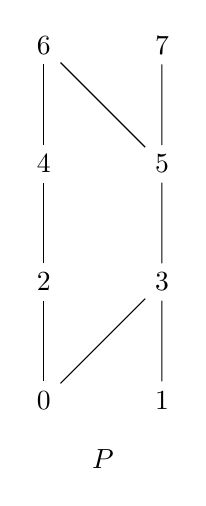
\begin{tikzpicture}[scale = .75]
  \node (0) at (0,0) {0};
  \node (1) at (2,0) {1};
  \node (2) at (0,2) {2};
  \node (3) at (2,2) {3};
  \node (4) at (0,4) {4};
  \node (5) at (2,4) {5};
  \node (6) at (0,6) {6};
  \node (7) at (2,6) {7};
  \draw (0)--(2);
  \draw (0)--(3);
  \draw (1)--(3);
  \draw (2)--(4);
  \draw (3)--(5);
  \draw (4)--(6);
  \draw (5)--(6);
  \draw (5)--(7);
  \node (8) at (1,-1) {$P$};
\end{tikzpicture}\qquad
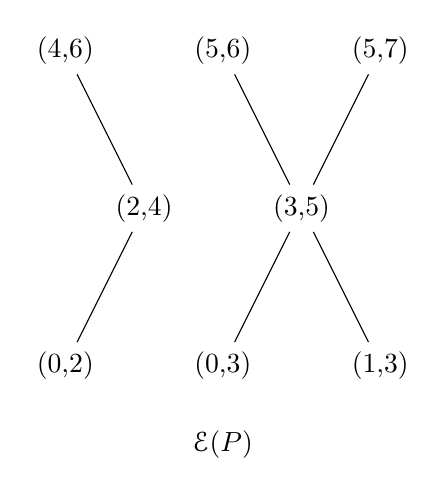
\begin{tikzpicture}
  \node (02) at (0,0) {(0,2)};
  \node (03) at (2,0) {(0,3)};
  \node (13) at (4,0) {(1,3)};
  \node (24) at (1,2) {(2,4)};
  \node (35) at (3,2) {(3,5)};
  \node (46) at (0,4) {(4,6)};
  \node (56) at (2,4) {(5,6)};
  \node (57) at (4,4) {(5,7)};
  \draw (02)--(24);
  \draw (03)--(35);
  \draw (13)--(35);
  \draw (24)--(46);
  \draw (35)--(56);
  \draw (35)--(57);
  \node (0) at (2,-1) {$\mathcal{E}(P)$};
\end{tikzpicture}
\caption{$P$ is self-dual and unitary Peck, but $\mathcal{E}(P)$ is not Peck}
\end{figure}


\begin{rem}
\label{rem:induced_action_bn}
Whenever there is an action $\psi:G \times [n] \rightarrow [n],$ we obtain an induced action $\phi: G \times B_n \rightarrow B_n$ defined by
$$\phi(g,\{x_1,\ldots, x_k\}) = \{\psi(g,x_1),\ldots, \psi(g,x_k)\}.$$
It is well known and easy to see that in fact any action $\phi:G \times B_n \rightarrow B_n$ arises in this way. That is, for any action $\phi$ of $G$ on $B_n$ there exists an action $\psi$ of $G$ on $[n]$ such that $\phi(g,\{x_1,\ldots, x_k\}) = \{\psi(g,x_1),\ldots, \psi(g,x_k)\}.$ Whenever an action $\psi$ of $G$ on $[n]$ is given, we shall refer to the action $\phi$ defined above as the induced action on $B_n.$
\end{rem}



\begin{cor}
For any action $\phi:G \times B_n \rightarrow B_n,$ both $\mathcal E(B_n/G)$ and $\mathcal E(B_n)/G$ are self-dual. In particular, they are both symmetric. 
\end{cor}
\begin{proof}
By Remark \ref{rem:induced_action_bn}, any action of $\phi$ of $G$ on $B_n$ is induced by an action $\psi:G \times [n] \rightarrow [n].$ Using this, observe that for any group action $G,$ the poset $B_n/G$ is self-dual, as there is an isomorphism $f:B_n/G \rightarrow (B_n/G)^{op},G \cdot x \mapsto G \cdot ([n] \setminus x).$ This map is well defined on $G$ orbits because every action on $B_n$ is induced by an action on $[n].$ Then, by Proposition \ref{prop:self_dual_preservation} it follows $\mathcal E(B_n/G)$ is self-dual, and in particular $\mathcal E(B_n)$ is self-dual.

It only remains to prove that $\mathcal E(B_n)/G$ is self-dual. However, we just saw $\mathcal E(B_n)$ is self-dual, with the isomorphism given by $\mathcal E(f):\mathcal E(B_n) \rightarrow \mathcal E(B_n^{op})\cong \mathcal E(B_n)^{op},$ that is, the map sending a pair of elements to the pair of their complements. Once again, since the action on $B_n$ is induced by an action on $[n],$ this isomorphism descends to an isomorphism $\mathcal E(f)^G:\mathcal E(B_n)/G \rightarrow \mathcal (E(B_n)/G)^{op},$ and so $\mathcal E(B_n)/G$ is self-dual.
\end{proof}


\ssec{Proof of Theorem \ref{thm:cover_transitive_implies_Peck}}\label{ssec:proof_of_cover_transitive_implies_Peck}

In this section we prove Theorem \ref{thm:cover_transitive_implies_Peck}, which we recall here:

\cctpeck*

The proof is largely motivated by the following Lemma.

\begin{lem}\label{lem:bijection_peck_implication}
If $f:P\rightarrow Q$ is a bijection (but not necessarily an isomorphism) and $P$ is Peck then $Q$ is Peck.
\end{lem}
\begin{proof}
Let $\rk(P) = \rk(Q) = n$.  Since $P$ is Peck there exists an order-raising operator $U$ such that $U^{n-2i}\colon P_i\rightarrow P_{n-i}$ is an isomorphism.  Since $f$ is a poset morphism, it follows that the map $f\circ U\circ f^{-1}$ is an order-raising operator on $Q$.  We then have that $f\circ U^{n-2i}\circ f^{-1} = \left(f\circ U\circ f^{-1}\right)^{n-2i}\colon Q_i\rightarrow Q_{n-i}$ is an isomorphism since $U^{n-2i}\colon P_i\rightarrow P_{n-i}$ is an isomorphism and $f$ is a bijection.

%Let $rk(P) = rk(Q) = n.$ Since $P$ is Peck, there exists an order raising map $U_i:P_i\rightarrow P_{i+1}$ such that $U_{n-i-1} \cdots U_i:P_i \rightarrow P_{n-i}$ is an isomorphism. Then, define $f(U)_i:P_i\rightarrow P_{i+1}$ by $f(U)_i(x) = f(U_i(f^{-1}(x))).$ This map is well defined because $f$ is a bijection. This map is order raising because $y > x \implies f(y) > f(x),$ by definition of morphisms of posets. It follows that since $U_{n-i-1} \cdots U_i$ is an isomorphism, $f(U)_{n-i-1} \cdots f(U)_i$ is as well, because the vector spaces $V(P_i) \cong V(Q_i)$ since $f$ is a bijection. Therefore, $Q$ is Peck.
\end{proof}

By Lemma \ref{lem:bijection_peck_implication} and Proposition \ref{prop:surjection_between_F_quotients}, in order to prove Theorem \ref{thm:cover_transitive_implies_Peck} it suffices to prove that $\mathcal E(B_n)/G$ is Peck.  One way to do this is to prove that $\mathcal E(B_n)$ is unitary Peck and then apply Theorem \ref{thm:quotients_of_unitary_peck_posets}. We prove that $\mathcal E(B_n)$ is unitary Peck in Section \ref{sec:unitary_peck_f}, but unfortunately the proof is messy and computational.


%At least for the case $r=1$ there is an alternative proof of this fact. It is actually shown in Section ~\ref{sec:unitary_peck_f} that $\mathcal E(B_n)$ is unitary Peck, for $n>2,$ so, by Theorem \ref{thm:quotients_of_unitary_peck_posets}, $\mathcal E(B_n)/G$ is Peck. However, the proof of this is extremely messy and computational.

Fortunately there is a simpler -- albeit less direct -- route.  In order to avoid showing that $\mathcal E(B_n)$ is unitary Peck, we define a graded poset $\mathcal{H}(B_n)$ for all $n$ such that $\mathcal{H}(B_n)$ is easily seen to be unitary Peck in Corollary \ref{cor:HBn_unitary_peck}. Furthermore, we define $\mathcal{H}(B_n)$ such that a group action of $G$ on $B_n$ induces a group action on $\mathcal{H}(B_n)$ (Lemma \ref{lem:G_action_on_HP}) and there is always a bijective morphism $f\colon \mathcal{H}(B_n)/G\rightarrow \mathcal E(B_n)/G$ (Lemma \ref{lem:bijection_h_f}).  By the above discussion, Theorem \ref{thm:cover_transitive_implies_Peck} readily follows.

\begin{defn}
\label{defn:h_map}
For $P$ a graded poset, define the graded poset $\mathcal H(P)$ as follows. Let the elements $(x, y) \in \mathcal H(P)$ to be pairs $(x,y) \in P\times P$ such that $x \lessdot y$.  Define $(x, y) \lessdot_{\mathcal H} (x^\prime, y^\prime)$ if $x \lessdot x^\prime,y\lessdot y^\prime$ and $x^\prime \neq y.$ Then, define $\leq_{\mathcal H}$ to be the transitive closure of $\lessdot_{\mathcal H}.$ and define $\rk_{\mathcal H}(x, y) = \rk_P(x).$
\end{defn}


\begin{eg}
\label{eg:3boolean}
We give an example of the poset $\mathcal H(B_3)$ in Figure \ref{fig:3boolean}. Observe that $\mathcal H(B_3)$ can be written as a disjoint union of three copies of $B_2.$ This is a single case of the more general phenomenon proven in Proposition \ref{prop:computing_HBn}.
\end{eg}

\begin{figure}[h!]
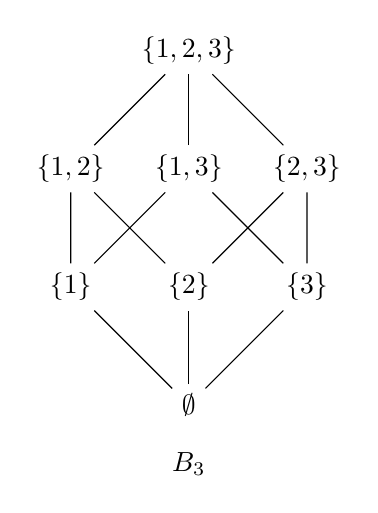
\begin{tikzpicture}[scale = 1.5]
  \node (0) at (0,0) {$\emptyset$};
  \node (1) at (-1,1) {$\{1\}$};
  \node (2) at (0,1) {$\{2\}$};
  \node (3) at (1,1) {$\{3\}$};
  \node (4) at (-1,2) {$\{1,2\}$};
  \node (5) at (0,2) {$\{1,3\}$};
  \node (6) at (1,2) {$\{2,3\}$};
  \node (7) at (0,3) {$\{1,2,3\}$};
  \draw (0)--(1);
  \draw (0)--(2);
  \draw (0)--(3);
  \draw (1)--(4);
  \draw (1)--(5);
  \draw (2)--(4);
  \draw (2)--(6);
  \draw (3)--(5);
  \draw (3)--(6);
  \draw (4)--(7);
  \draw (5)--(7);
  \draw (6)--(7);
  \node (8) at (0,-.5) {$B_3$};
\end{tikzpicture} 

\vspace*{0.3in}

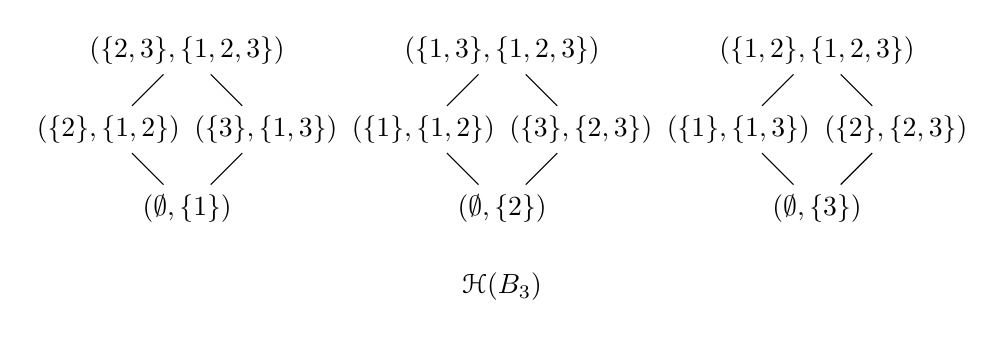
\begin{tikzpicture}[scale = 1]
  \node (0) at (0,0) {$(\emptyset,\{1\})$};
  \node (1) at (4,0) {$(\emptyset,\{2\})$};
  \node (2) at (8,0) {$(\emptyset,\{3\})$};
  \node (3) at (3,1) {$(\{1\},\{1,2\})$};
  \node (4) at (7,1) {$(\{1\},\{1,3\})$};
  \node (5) at (-1,1) {$(\{2\},\{1,2\})$};
  \node (6) at (9,1) {$(\{2\},\{2,3\})$};
  \node (7) at (1,1) {$(\{3\},\{1,3\})$};
  \node (8) at (5,1) {$(\{3\},\{2,3\})$};
  \node (9) at (8,2) {$(\{1,2\},\{1,2,3\})$};
  \node (10) at (4,2) {$(\{1,3\},\{1,2,3\})$};
  \node (11) at (0,2) {$(\{2,3\},\{1,2,3\})$};
  \draw (0)--(5)--(11)--(7)--(0);
  \draw (1)--(3)--(10)--(8)--(1);
  \draw (2)--(4)--(9)--(6)--(2);
  \node (12) at (4,-1) {$\mathcal{H}(B_3)$};
\end{tikzpicture}
\caption{\label{fig:3boolean} $B_3$ and $\mathcal H (B_3)$}
\end{figure}


\begin{rem}\label{rem:order_containment}
Note that by definition $(x,y)\lessdot_{\mathcal{H}} (x^\prime,y^\prime)$ precisely when $(x,y)\lessdot_{\mathcal{E}} (x^\prime,y^\prime)$ and $x^\prime\neq y$, hence $(x, y)\lessdot_{\mathcal{H}} (x^\prime, y^\prime) \Rightarrow (x, y)\lessdot_{\mathcal E} (x^\prime, y^\prime)$.  In other words, $\mathcal{H}(P)$ has the same elements as $\mathcal{E}(P)$ but with a weaker partial order.
\end{rem}


\begin{lem}\label{lem:HP_order}
For $P$ a graded poset, the object $\mathcal{H}(P)$, as defined in Definition ~\ref{defn:h_map} is a graded poset.
\end{lem}

\begin{proof}
This follows immediately from Remark \ref{rem:order_containment} and the fact that $\mathcal E(P)$ is graded.
\end{proof}
%To show $\mathcal H(P)$ is graded, we must show $x\otimes y <_{\mathcal H} a \otimes b \implies rk(x\otimes y)<rk(a \otimes b)$ and $x\otimes y \lessdot_{\mathcal H} a \otimes b \implies rk(x\otimes y)+1 = rk(a \otimes b).$ 

%First, if $x\otimes y <_{\mathcal H} a \otimes b$ then by definition of $<_{\mathcal H},$ in Definition ~\ref{defn:h_map}, we must have $x < a,$ and hence 
%$$rk_{\mathcal H(P)}(x\otimes y) = rk_P(x)<rk_P(a) = rk_{\mathcal H(P)}(a\otimes b).$$
%Second, if $x\otimes y \lessdot_{\mathcal H} a \otimes b$ then $x \lessdot_P a,$ so $rk(x)+1 = rk(a)$ and then $$rk_{\mathcal H(P)}(x\otimes y)+1 = rk_P(x) +1=rk_P(a)= rk_{\mathcal H(P)}(a\otimes b).$$

\begin{rem}
While $\mathcal E:\mathcal P \rightarrow \mathcal P$ is a functor, $\mathcal H$ is not a functor. In particular, we have not specified how $\mathcal H$ acts on morphisms. If, for $f:P \rightarrow Q,$ we attempted to define $\mathcal H(f):\mathcal H(P) \rightarrow \mathcal H(Q),$ we would quickly run into trouble. For example, suppose we took $f$ mapping a diamond $P$ (see Figure \ref{fig:h_morphism}) to a chain of length three $Q$. Then, $\mathcal H(P)$ has four points, with two pairs of edges, whereas $\mathcal H(Q)$ has two disconnected points. It is clear that there can be no order-preserving mapping between these two objects.

\todo{anyone know how to align these evenly?}
\begin{figure}[h!]
\label{fig:h_morphism}
\begin{center}
\begin{tikzpicture}[scale=.7]
  \node (b) at (0:2cm) {$3$};
  \node (a) at (90:2cm) {$4$};
  \node (c) at (180:2cm) {$2$};
  \node (d) at (270:2cm) {$1$};
  \draw (a) -- (b) -- (d) -- (c)--(a);
  \node (e) at (270:3cm) {$P$};
\end{tikzpicture}\quad
\begin{tikzpicture}[scale=.7]
  \node (b) at (90:2cm) {$3$};
  \node (a) at (270:2cm) {$1$};
  \node (c) at (0:0cm) {$2$};
  \draw (a) -- (c) -- (b);
  \node (e) at (270:3cm) {$Q$};
\end{tikzpicture}\quad
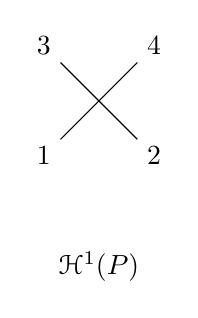
\begin{tikzpicture}[scale=.7]
  \node (b) at (45:1.414cm) {$4$};
  \node (a) at (135:1.414cm) {$3$};
  \node (c) at (225:1.414cm) {$1$};
  \node (d) at (315:1.414cm) {$2$};
  \draw (a) -- (d) ;
  \draw (c) -- (b);
  \node (e) at (270:3cm) {$\mathcal{H}^1(P)$};
\end{tikzpicture} \quad
\begin{tikzpicture}[scale=.7]
  \node (b) at (90:1cm) {$2$};
  \node (a) at (270:1cm) {$1$};
  \node (e) at (270:3cm) {$\mathcal{H}^1(Q)$};
\end{tikzpicture}
\end{center}
\caption{}
\end{figure}
\end{rem}



Given an action of a group $G$ on $P$, we define an action of $G$ on $\mathcal{H}(P)$ as we did for $\mathcal{E}(P)$ by again defining $g\cdot (x,y) = (gx,gy)$ for all $(x,y)\in P$.  We will then have a well-defined quotient poset $\mathcal{H}(P)/G$ with the same elements as $\mathcal{E}(P)/G$.


\begin{lem}
\label{lem:G_action_on_HP}
The function defined by $g\cdot (x, y)= (gx, gy)$ for all $g\in G$, $(x, y)\in \mathcal{H}(P)$ is a well-defined group action of $G$ on $\mathcal{H}(P)$.
\end{lem}

\begin{proof}
Let $g\in G$.  Since $\le_{\mathcal{H}}$ is the transitive closure of $\lessdot_{\mathcal{H}}$ it suffices to show that for all $(x,y),(x^\prime,y^\prime)\in \mathcal{H}(P)$ we have $(x, y) \lessdot_{\mathcal H} (x^\prime,y^\prime) \iff g(x, y) \lessdot_{\mathcal H} g(x^\prime, y^\prime)$.  Since $g$ is an automorphism of $P$, we have $x\le_P x^\prime \iff gx\le_P gx^\prime$, $y\le_P y^\prime \iff gy\le_P gy^\prime$, and $y\neq x^\prime \iff gy\neq gx^\prime$, so the result follows from the definition of $\le_{\mathcal{H}}$.
\end{proof}
%It is rank preserving because $$rk_{\mathcal H(P)}(g\cdot(x, y)) = rk_{\mathcal H(P)}(gx, gy)) = rk_P(gx)=rk_P(x) = rk_{\mathcal H(P)}(x, y).$$

%The fact that the $G$-action is rank-preserving on $\mathcal{H}(P)$ follows from the fact that $G$-action is rank-preserving on $\mathcalH(P)$.  In order to show the action is order preserving, it suffices to show that if $(x, y) \lessdot_{\mathcal H} (a, b)$ then $g(x, y) \lessdot_{\mathcal H} g(a, b),$ because $\leq_{\mathcal H}$ is the transitive closure of $\lessdot_{\mathcal H}.$ By definition of $\lessdot_{\mathcal H},$ we have $x \lessdot_P a,y\lessdot_P b,y \not \leq b$.  Since $g$ is an automorphism of $P$ for all $g\in G$, it follows that $gx \lessdot_P ga,gy \lessdot_P gb, gy \not \leq_P gb$, hence $g(x, y) \lessdot_{\mathcal H} g(a , b).$






\begin{lem}
\label{lem:bijection_h_f}
The map $f:\mathcal H(P)/G \rightarrow \mathcal E(P)/G$ defined by $G(x,y) \mapsto G(x,y)$ is a bijection for any group action of $G$ on $P$.
%Took part below out because it's not true and because I'm not sure how helpful the true version is - David
%(but never an isomorphism for $n-r > 1$)
\end{lem}

\begin{proof}
The elements of $\mathcal H(P)/G,\mathcal E(P)/G$ are the same by definition. Therefore, as long as $f$ is a morphism, it is automatically a bijection. Since $f$ is clearly rank-preserving, to show $f$ is a morphism, it suffices to show $f$ is order-preserving. This is immediate from Remark ~\ref{rem:order_containment}.
\end{proof}

The remaining ingredient to the proof of Theorem \ref{thm:cover_transitive_implies_Peck} is to show that $\mathcal{H}(B_n)$ is unitary Peck, which we do by generalizing Example \ref{eg:3boolean} and showing that $\mathcal{H}(B_n)$ is isomorphic to the disjoint union of boolean algebras.

\begin{prop}\label{prop:computing_HBn}
$\mathcal{H}(B_n)$ is isomorphic to $n$ disjoint copies of $B_{n-1}$.
\end{prop}

\begin{proof}

Suppose we have $(x, y),(x', y') \in \mathcal H(B_n)$ with $(x, y) \lessdot (x', y').$ Let $j\in [n]$ such that $y^\prime = y\cup\{j\}$, and let $i\in [n]$ such that $x^\prime = x\cup \{i\}$. If $i \ne j,$ then $x' \leq y,$ contradicting the assumption that $(x, y) \lessdot_{\mathcal H} (x', y').$ Thus $x^\prime = x\cup\{i\}$ and $y^\prime = y\cup\{i\}$ for some $i\in [n]$.

Conversely we can easily check that if $i\not\in y$, then $(x, y)\lessdot_{\mathcal{H}} (x\cup\{i\}, y\cup\{i\})$.  It follows that for all subsets $w \subset [n]$ such that $|w| = 1$, there is an isomorphism from the subposet of elements $\{(x, y)\colon y\setminus x = w\}$ to $B_{n-1}$ defined by $(x,y)\mapsto (x\setminus w,y\setminus w)$.  Furthermore if $y\setminus x \ne y^\prime \setminus x^\prime$, then $(x, y)$ and $(x^\prime, y^\prime)$ are incomparable, so these subposets indexed by $w$ are pairwise disjoint, and $\mathcal H(B_n)$ is isomorphic to $n$ copies of $B_{n}$.
\end{proof}

\begin{cor}\label{cor:HBn_unitary_peck}
$\mathcal H(B_n)$ is unitary Peck for all $n\ge 0$.
\end{cor}

\begin{proof}
This follows immediately from Proposition \ref{prop:computing_HBn} and the fact that $B_{n-1}$ is unitary Peck.  The latter is shown, for instance in \cite[Theorem 2a]{quotients_stanley} by noting that $B_k = (B_1)^k$ and that $B_1$ is clearly unitary Peck.
\end{proof}

\begin{cor}\label{cor:quotients_of_HBn_peck}
$\mathcal H(B_n)/G$ is Peck for any subgroup $G\subset S_n$.
\end{cor}

\begin{proof}
This follows from Corollary \ref{cor:HBn_unitary_peck} and Theorem \ref{thm:quotients_of_unitary_peck_posets}.
\end{proof}




\begin{cor}
\label{cor:quotiented_edge_peck}
$\mathcal E(B_n)/G$ is Peck for any subgroup $G\subset S_n$.
\end{cor}
\begin{proof}
By Corollary ~\ref{cor:quotients_of_HBn_peck}, $\mathcal H(B_n)/G$ is Peck. By Lemma ~\ref{lem:bijection_h_f}, the map $f:\mathcal H(P) \rightarrow \mathcal E(P),G(x, y) \mapsto G(x, y)$ is a bijection. Then, by Lemma ~\ref{lem:bijection_peck_implication}, it follows that $\mathcal E(B_n)/G$ is Peck.
\end{proof}

\begin{proof}[Proof of Theorem \ref{thm:cover_transitive_implies_Peck}]
By Corollary \ref{cor:quotiented_edge_peck}, $\mathcal{E}(B_n)/G$ is Peck for any group action of $G$ on $B_n.$ Since the $G$-action is CCT, there is a bijective morphism from $\mathcal{E}(B_n)/G$ to $\mathcal{E}(B_n/G)$, hence $\mathcal{E}(B_n/G)$ is Peck by Lemma \ref{lem:bijection_h_f}.
\end{proof}


\subsection{A Generalization of $\mathcal H,\mathcal E$}\label{ssec:E_generalization}

Although for the most part, we shall investigate \linebreak
$\mathcal E(P/G),\mathcal E(P)/G,$ there is a natural generalization of $\mathcal E,\mathcal H,$ to what we shall call $\mathcal E^{\vec r},\mathcal H^{\vec r},$ where $\vec r = r_1,r_2,\ldots, r_k$ is an integer valued sequence. The results holding for these generalizations are analogous to those developed above. The purpose of developing these generalizations notion will be to give a more general application to Polya theory than could be given with $\mathcal E.$

\begin{defn}
Let $\vec r = r_1,\ldots,r_k.$ For a graded poset $P,$ define the graded poset $\mathcal H^{r_1,\ldots, r_k}(P),$ also notated $\mathcal H^{\vec r}(P),$ whose elements are formal symbols $(x_1, x_2, \cdots, x_{k+1})$ such that $rk(x_i)+r_i = rk(x_{i+1}),$ for all $i \in [k].$ Say 
$$(x_1, x_2, \cdots, x_{k+1})\lessdot_{\mathcal H^{\vec r}} (y_1, y_2, \cdots, y_{k+1})$$
if $x_i \lessdot_P y_i,y_{i} \not \leq_P x_{i+1}$ for all $i \in [k+1].$ Then, define a relation $<_{\mathcal H^{\vec r}}$ on $\mathcal H^{r_1,\ldots, r_k}(P),$ to be the transitive closure of $\lessdot_{\mathcal H^{\vec r}}.$ Finally, define 
$$rk_{\mathcal H^{\vec r}(P)}(x_1,\ldots, x_{k+1}) = rk_P(x_1).$$
\end{defn}

\begin{defn}
Let $\vec r = r_1,\ldots,r_k,$ with $r_i \in \BN$ for all $i \in [k].$ Let $\mathcal P$ be the category of graded posets. Define the functor $\mathcal E^{\vec r}:\mathcal P \rightarrow \mathcal P,$ also notated $\mathcal E^{r_1,\ldots, r_k}.$ For a graded poset $P,$ define the graded poset $\mathcal E^{r_1,\ldots, r_k}(P),$ also notated whose elements are formal symbols $(x_1, x_2, \cdots, x_{k+1})$ such that $rk(x_i)+r_i = rk(x_{i+1}),$ for all $i \in [k].$ Say 
$$(x_1, x_2, \cdots, x_{k+1})\lessdot_{\mathcal H^{\vec r}} (y_1, y_2, \cdots , y_{k+1})$$ if $x_i \lessdot_P y_i$ for all $i \in [k+1]$. Then, define a relation $\leq_{\mathcal E^{\vec r}}$ on $\mathcal E^{r_1,\ldots, r_k}(P),$ to be the transitive closure of $\lessdot_{\mathcal E^{\vec r}}.$ Finally, define 
$$rk_{\mathcal E^{\vec r}(P)}(x_1,\ldots, x_{k+1}) = rk_P(x_1).$$
\end{defn}

Observe that under this notation, $\mathcal E^1 = \mathcal E, \mathcal H^1 = \mathcal H.$

\begin{rem}
For all $\vec r,\mathcal E^{\vec r}$ is a functor, for the same reasons that $\mathcal E$ is a functor. This generalization is essentially taking the nerves of the poset $P.$ See \cite{babson} for some related constructions, although their constructions are not completely analogous.
\end{rem}

In the next Lemmas, we cite analogous results which hold for $\mathcal H^{\vec r}.$ The proofs are almost identical to those for $\mathcal H.$

\begin{lem}
Given a group action $\phi:G \times P \rightarrow P$ there are well defined group actions 
$$\phi_{\mathcal E}:G\times \mathcal E^{\vec r}(P) \rightarrow \mathcal E^{\vec r}(P),$$
$$\phi_{\mathcal H}:G\times \mathcal H^{\vec r}(P) \rightarrow \mathcal H^{\vec r}(P),$$ 
both given by 
$$g \cdot (x_1, \cdots, x_{k+1}) =(g\cdot x_1, \cdots, g \cdot x_{k+1}).$$
\end{lem}
\begin{proof}
The proof is analogous to that of Lemma ~\ref{lem:G_action_on_HP}.
\end{proof}

\begin{lem}
\label{lem:peck_quotients_vector_f}
The poset $\mathcal H^{r_1,\ldots, r_k}(B_n)$ is isomorphic to the multinomial coefficient \linebreak $\binom n {r_1,r_2,\ldots, r_k}$ disjoint copies of $B_{n- \sum_{i=1}^k r_i}.$ Consequently, $\mathcal H^{\vec r}(B_n)$ is unitary Peck and \linebreak
$\mathcal H^{\vec r}(B_n)/G$ is Peck.
\end{lem}
\begin{proof}
Once again, the proof of the above three statements is analogous to those of ~\ref{prop:computing_HBn}, Corollary ~\ref{cor:HBn_unitary_peck}, and Corollary ~\ref{cor:quotients_of_HBn_peck}. The reason there are multinomial coefficients here instead of binomial coefficients, is that an element $(x_1, x_2, \cdots, x_{k+1})$ lies in the copy of $B_{n -\sum_{i=1}^k r_i}$ determined by the ordered tuple of subsets $(x_2 \setminus x_1,x_3 \setminus x_2, \ldots, x_{k+1} \setminus x_k).$ The first consists of $r_1$ elements, the next of $r_2$ elements, up through the last which consists of $r_k$ elements. Since the total number of ways to choose $r_1,\ldots, r_k$ in $k$ distinct groups is $\binom n {r_1,r_2,\ldots, r_k},$ there are exactly this many disjoint copies of $B_{n- \sum_{i=1}^k r_i}.$
\end{proof}





%%%%%%%%%%%%%%%%%  CCT actions  %%%%%%%%%%%%%%%%%%
\section{Common Cover Transitive Actions}
\label{sec:cover_transitive}
In this section, we develop the theory of CCT actions $\phi$ where $G$ is a group, $P$ is a poset, and $\phi:G\times P \rightarrow P$ is an action. Recall Definition ~\ref{defn:cover_transitive}, that $\phi$ is CCT if whenever $x,y,z \in P,x\lessdot y,y\lessdot z,x \in Gy$ then there exists $g \in Stab(z)$ with $gx = y.$ For CCT actions $\phi:G\times P \rightarrow P,$ we shall show that, $\mathcal E(P/G)$ is Peck. Additionally, we shall show the CCT property is closed under semidirect products, in the appropriate sense. From Proposition ~\ref{prop:cover_transitive_building_blocks}, which shall be proven in subsection \ref{ssec:dihedral}, the action of $S_n$ on $B_n$ and the action of certain dihedral groups are CCT. We can then use these as building blocks to construct other CCT groups. In particular, we shall show in this section that automorphism groups of rooted trees are CCT.

\begin{rem}
Before continuing with the description of cover transitive, it is worth noting that the notion of cover transitivity generalizes to $\mathcal E$ and even $\mathcal E^{\vec r}.$ Letting $\vec r = r_1,\ldots, r_k,$ one would call a group action $\phi:G\times P \rightarrow P,$ {\it $\vec r$ common cover transitive} if for any chains $(x_0,\ldots, x_k),(y_0,\ldots, y_k),$ such that there exists $g_i \in G$ with $x_i = g_i y_i,$ for all $i,0\leq i \leq k,$ then there exists a single $g \in G$ with $x_i = g y_i.$ It is trivial to see that $1$ common cover transitive agrees with our definition of common cover transitive. Furthermore, it is also simple to see that an action is $\vec r$ common cover transitive if and only if the natural surjection $q:\mathcal E^{\vec r}(P)/G \rightarrow \mathcal E^{\vec r}(P/G)$ is a bijection. Additionally, very many of the properties developed in this section will also hold for this generalized notion of $\vec r$ common cover transitive.
\end{rem}

\begin{eg}
\label{eg:trivial_edgequot}
Two rather trivial examples of CCT actions are $\phi:S_n\times B_n \rightarrow B_n,\psi:G\times B_n\rightarrow B_n$ where $G$ is arbitrary, $\phi$ is the action induced by $S_n$ permuting the elements of $[n]$, and $\psi$ is the trivial action. In the former case, $\mathcal E(B_n/S_l)$ is simply a chain with $n-1$ points, and so is $\mathcal E(B_n)/S_l,$ since all $(x, y)$ are identified under the $S_l$ action. In the latter case, since $G$ acts trivially by $\phi,$ both  $\mathcal E(B_n/G) \cong \mathcal E(B_n)$ and $\mathcal E(B_n)/G \cong \mathcal E(B_n).$ So again, $\psi$ is CCT.
\end{eg}

\begin{thm}
If an action $\phi:G \times P \rightarrow P$ is CCT, and $\mathcal E(P)$ is Peck, then $\mathcal E(P/G)$ is Peck.
\end{thm}
\begin{proof}
By Proposition ~\ref{prop:surjection_between_F_quotients}, there is a surjection $q:\mathcal E(P)/G \rightarrow \mathcal E(P/G).$ Additionally, by Lemma ~\ref{prop:surjection_between_F_quotients}, if $\phi$ is CCT, $q$ is a bijection. Finally, by Lemma ~\ref{lem:bijection_peck_implication}, since $q:\mathcal E(P)/G \rightarrow \mathcal E(P/G)$ is a bijection and $\mathcal E(P)/G$ is Peck, it follows that $\mathcal E(P/G)$ is Peck.
\end{proof}


\ssec{Preservation Under Semidirect Products}
\label{ssec:semidirect_product_preservation}
Recall Proposition ~\ref{prop:semidirect_product_preservation}, as stated in the introduction. This Proposition essentially says the CCT property is preserved under semidirect products. We shall use this to obtain simple proofs that CCT actions are also preserved under direct products and wreath products.

\semidirect*

\begin{proof}
Since $G = H\rtimes K$, every element $g\in G$ can be written uniquely as a product $hk$ for some $h\in H$, $k\in K$.  Let $x,y,z\in P$ such that $x\lessdot z$, $y\lessdot z$ and such that there exists some $h_0k_0\in G$ such that $h_0k_0\cdot x = y$.  It suffices to show that there exists some $g\in \Stab(z)$ such that $g\cdot x = y$.

The orbits $Hx, Hy, Hz\in P/H$ satisfy $Hx\lessdot Hz$, $Hy\lessdot Hz$ such that $k_0\cdot Hx = Hy$, so since the action of $K$ on $P/H$ is CCT there exists some $k_1\in K$ such that $k_1\in \Stab(Hz)$ and $k_1\cdot Hx = Hy$.  It follows that there exists some $h_1\in H$ such that $h_1k_1h_0\in \Stab(z)$ and $h_1k_1h_0\cdot x\in Hy$.

Write $x^\prime = h_1k_1h_0\cdot x$.  Since the group action of $G$ must be order-preserving by definition, we have that $x^\prime \lessdot z$.  We already had that $y\lessdot z$ and $x^\prime\in Hy$, hence there exists some $h_2\in \Stab(z)$ such that $h_2\cdot x^\prime = y$ by the fact that the action of $H$ on $P$ is CCT.  Then we have that $h_2h_1k_1h_0\cdot x = h_2\cdot x^\prime = y$ and $h_2h_1k_1h_0\cdot z = h_2\cdot z = z$, as desired.
\end{proof}

\begin{prop}
\label{prop:direct_product_preservation}
For $\phi:G\times P\rightarrow P,\psi:H \times Q \rightarrow Q$ two CCT actions, then the direct product 
$$\phi \times \psi:(G\times H)\times (P\times Q) \rightarrow (P\times Q),(g,h)\cdot (x,y) \mapsto (gx,hy)$$
is also CCT.
\end{prop}
\begin{proof}
First, by definition of CCT, if either $G$ or $H$ acts trivially, it is clear the action of $G\times H$ is CCT. To see this, suppose $G$ acts trivially, the case of $H$ acting trivially is similar. Then, if $(x,y) \lessdot (a,b),(r,s)\lessdot (a,b),(x,y) \in (G\times H)(r,s),$ then $x \in Gr$ so $x = r.$ There are now two cases, either $b = y = s$ or $x = r = a.$ First, if $b = y = s,$ then $(e,e) \in Stab(x,y)$ and $(e,e)(x,y) = (r,s).$ Second, if $x = r = a,$ and then $y \lessdot b,s \lessdot b,y \in Hs,$ and so by cover transitivity of $G,$ there exists $g \in G$ so that $(e,g)(x,y) = (r,s)$ and $(e,g) \in Stab(a,b).$

Next, Observe that $G \times H$ can be viewed as the semidirect product of $(G\times \{e\}) \rtimes (\{e\} \times H).$ Since the action of $G$ on $P$ is CCT, by the above paragraph, the action of $G\times \{e\}$ on $P \times Q$ is CCT. Also, since the action of $H$ on $Q$ is CCT, it follows that the action of $\{e\}\times H$ on $(P/G) \times Q$ is CCT. Therefore, the action of $(G\times \{e\}) \rtimes (\{e\} \times H)$ satisfies the conditions of Proposition ~\ref{prop:semidirect_product_preservation} and so the action of $G\times H$ is CCT.
\end{proof}

Next, we use Proposition ~\ref{prop:semidirect_product_preservation} to prove in Proposition ~\ref{prop:wreath_preservation} that the CCT property is preserved under wreath products with the symmetric group. First, we need some definitions of wreath product.

\begin{defn}
For $G, H$ groups, with $H \subset S_l,$ the {\it wreath product}, notated $G \wr H,$ is the group whose elements are pairs $(g,h) \in G^l\times H$ with multiplication defined by
\begin{align*}
((g_1',\ldots, g_l'),h') \cdot ((g_1,\ldots, g_l) ,h) =((g'_{h'(1)}g_1,\ldots, g'_{h'(l)}g_l),hh')
\end{align*}
where $h \in H$ acts on $[l]$ by the restricting of the action of $S_l$ on $[l]$ by all permutations to $H.$
\end{defn}

In other words, $G\wr H$ can be viewed as a certain semidirect product of $G^l \rtimes H.$

\begin{note}
\label{note:wreath_action}
For any group $G$ with a given action $\psi:G\times P \rightarrow P,$ we obtain an induced action of $G \wr H,$ $\phi:G \wr H \times P^l \rightarrow P^l$ defined by 
$$((g_1,\ldots, g_l),h)(a_1,\ldots, a_l) = (g_{h^{-1}(1)}\cdot a_{h^{-1}(1)},\ldots,g_{h^{-1}(l)} \cdot a_{h^{-1}(l)}).$$
\end{note}

\begin{rem}
Heuristically, one may think of the above action as obtained by first having $G$ act separately on the $l$ distinct copies of $P,$ and then letting $H$ act by permuting the copies.
\end{rem}

\begin{lem}
\label{lem:symmetric_group_product_action}
For $P$ a poset, the action 
$$\phi:S_l \times P^l \rightarrow P^l,\sigma \cdot(x_1,\ldots, x_l) = (x_{\sigma(1)},\ldots, x_{\sigma(l)})$$
is CCT.
\end{lem}
\begin{proof}
For $a \in P^l$ notate $a = (a_1,\ldots, a_l).$ Suppose $x,y,z \in P^l$ with $x\lessdot z,y\lessdot z,$ and $x \in S_ly.$ This means there is a unique $i$ such that $x_i \lessdot z_i,x_k = z_k$ for $k \neq i.$ Additionally, there is a unique $j$ for which $y_j \lessdot z_j,y_k =z_k$ for $k \neq j.$ Since $x \in S_ly,$ we obtain the equality of multisets $\{x_1,\ldots, x_l\}=\{y_1,\ldots,y_l\}.$ But for $k \neq i,j,x_k = z_k = y_k$, we also obtain equality of sets $\{x_i,x_j\} = \{y_i,y_j\}.$ Since $rk(y_j) \lessdot rk(x_j),$ we obtain $y_j = x_i,y_i = x_j.$ Then, taking the transposition $\sigma  = (ij) \in S_l,$ it follows that $\sigma \in Stab(z)$ and $\sigma \cdot x = y.$
\end{proof}

\begin{prop}
\label{prop:wreath_preservation}
If $\psi:G\times P \rightarrow P$ is CCT, then $\phi:G\wr S_l \times P^l \rightarrow P^l$ where $\phi$ is the induced action defined in Notation \ref{note:wreath_action} is also CCT.
\end{prop}
\begin{proof}
First, the wreath product $G \wr S_l$ can be viewed as the semidirect product $G^l \rtimes S_l.$ Observe that since the action of $G$ on $P$ is CCT, using Proposition ~\ref{prop:direct_product_preservation}, we obtain the action of $G^l$ on $P^l$ is CCT. Explicitly, this action is $(g_1,\ldots, g_l)(x_1,\ldots, x_l) = (g_1 \cdot x_1,\ldots, g_l \cdot x_l).$ Additionally, since $P^l/G^l \cong (P/G)^l.$ So, for $\sigma \in S_l,x_i \in P/G,$ the action $S_l \times (P/G)^l \rightarrow (P/G)^l,(\sigma ,(x_1,\ldots, x_l)) \mapsto (x_{\sigma(1)},\ldots, x_{\sigma(l)})$ is CCT by Lemma ~\ref{lem:symmetric_group_product_action}. So, the action $\phi,$ satisfies the conditions of Proposition ~\ref{prop:semidirect_product_preservation} and so $\phi$ is CCT.
\end{proof}

\ssec{Examples of Cover Transitive Actions}\label{ssec:CCT_examples}

In this subsection, we describe several classes of cover transitive actions. First, we show that the automorphism group of any rooted tree is cover transitive. Second, we show linear automorphisms of simplices and octahedra are cover transitive. Third, we show that the left multiplication action is cover transitive if and only if the group is $\BZ_2^k,$ and that any action of $\BZ_2^k$ on $[n]$ induces a cover transitive action on $B_n.$

\sssec{An application to rooted trees}
\label{ssec:rooted_trees}
In this subsubsection, we prove that the automorphism group of rooted trees is always CCT. To do this we will apply Proposition ~\ref{prop:wreath_preservation} and Proposition ~\ref{prop:direct_product_preservation}, since the automorphism group of rooted trees is essentially built from direct products and wreath products with a symmetric group. To this aim, we first give definitions relating to rooted trees, then characterize their automorphisms, and finally show that such automorphism groups are always CCT. Our examination of of rooted trees automorphisms here, together with the examination of polytopes in subsubsection \ref{sssec:polytopes} was somewhat motivated by \cite[Section 5]{permutation_polytopes}.

\begin{defn}
A graded poset $P$ is a {\it rooted tree} if there is a unique element $x \in P$ of maximal rank, called the {\it root}, and for all $x \in P,$ other than the root, there exists a unique $y \in P$ with $y \gtrdot x.$
\end{defn}

\begin{eg}
In Figure \ref{fig:tree1} and Figure \ref{fig:tree2}, we give two examples of rooted trees.
\end{eg}

\begin{figure}[h!]
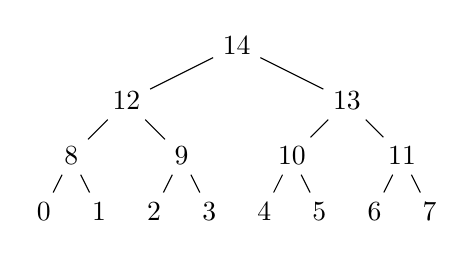
\begin{tikzpicture}[scale=.7]
  \node (0) at (-4,0) {$0$};
  \node (1) at (-3,0) {$1$};
  \node (2) at (-2,0) {$2$};
  \node (3) at (-1,0) {$3$};
    \node (4) at (0,0) {$4$};
  \node (5) at (1,0) {$5$};
  \node (6) at (2,0) {$6$};
  \node (7) at (3,0) {$7$};
  \node (8) at (-3.5,1) {$8$};
  \node (9) at (-1.5,1) {$9$};
  \node (10) at (.5,1) {$10$};
  \node (11) at (2.5,1) {$11$};
    \node (12) at (-2.5,2) {$12$};
  \node (13) at (1.5,2) {$13$};
  \node (14) at (-.5,3) {$14$};
  \draw (0)--(8);
  \draw (1)--(8);
  \draw (2)--(9);
  \draw (3)--(9);
  \draw (4)--(10);
  \draw (5)--(10);
  \draw (6)--(11);
  \draw (7)--(11);
  \draw (8)--(12);
  \draw (9)--(12);
  \draw (10)--(13);
  \draw (11)--(13);
  \draw (12)--(14);
  \draw (13)--(14);
\end{tikzpicture}
\caption{\label{fig:tree1}}
\end{figure}

\todo{Add this picture and example}
\begin{figure}[h!]
Add picture
\caption{\label{fig:tree2}}
\end{figure}

\begin{defn}
For $P$ a rooted tree, an element $x \in P$ is a {\it leaf} if there is no $z \in P$ with $x > z.$ Denote the set of all leaves of $P$ by $L(P).$
\end{defn}

\begin{lem}
\label{lem:induced_tree_action}
Let $P$ be a rooted tree. Then, the action of $Aut(P)$ on $P$ induces an action of $Aut(P)$ on $L(P).$ Furthermore, there is also an induced action of $Aut(P)$ on $B_n$ where $n = |L(P)|.$ 
\end{lem}
\begin{proof}
First, we must show that $Aut(P)$ induces an action on $L(P).$ That is, we must show that for any $g \in Aut(P),x \in L(P),$ then $gx \in L(P).$ If $x \in L(P)$ but $gx \notin L(P),$ then there exists $y < gx.$ However, then $g^{-1}y < x,$ contradicting the assumption that $x$ is a leaf. We then obtain the induced action $Aut(P)\times L(P) \rightarrow L(P),(g,x)\mapsto gx.$

Finally, to obtain the induced action of $Aut(P)$ on $B_n$ identify $L(P) \cong [n]$ as sets, where $|L(P)| = n$, and from this we get of action of $Aut(P)$ on $B_n.$
\end{proof}

\begin{convention}
For the rest of this section only, fix a rooted tree $P$ and denote by $G$ the group of automorphisms $Aut(P).$ Let $G$ act on $B_n,$ where $n = |L(P)|$ by the induced action $\phi:G \times P \rightarrow P,$ given by restricting $Aut(P)$ to $Aut(L(P)),$ as described in the proof of Claim ~\ref{lem:induced_tree_action}.
\end{convention}

\begin{note}
For $x \in P,$ denote $D(x) = \{y \in P: y \leq x\}.$
\end{note}
\begin{prop}
\label{prop:automorphism_trees}
Let $P$ be a rooted tree with root vertex labeled $r$. Let $\{A_1,\ldots,A_m\}$ denote the set of isomorphism classes of $\{D(x):x\lessdot r\}.$ For $T \in A_j,$ denote $G_j = Aut(T).$ Then, 
\begin{equation}
\label{eq:level_expansion}
Aut(P) = (G_1 \wr S_{i_1}) \times (G_2 \wr S_{i_2}) \times \cdots \times (G_m\wr S_{i_m}),
\end{equation}
In particular, $Aut(P)$ can be expressed as a sequence of direct products and wreath products of symmetric groups.
\end{prop}

\begin{proof}
It is clear that if $P$ is rank 0, then $Aut(P)$ is trivial. So, let us proceed by induction. That is, label the vertices of $P$ by $\{0,1,\ldots, s\}$ such that the root is labeled $0$ and the vertices just below the root are labeled $1, \ldots, k.$ Let $A_1,\ldots, A_m$ denote the distinct isomorphism classes of trees in the set $\{D(1),\ldots, D(k)\}.$ For $T \in A_j,$ denote $G_j = Aut(T).$ 
Let $T_j = \{t:t\lessdot 0,D(t) \cong A_j\}.$ Then, letting $Q_j$ be the subtree of $P$ whose elements lie in the set $0 \cup (\cup_{t \in T_j} D(t)),$ it follows $Aut(Q_j) \cong G_j \wr S_{i_j},$ because after choosing a permutation of the elements of $T_j,$ we are free to choose any element of $G_j$ to permute each $D(t),t \in T_j$. If $t_1 \lessdot 0,t_2 \lessdot 0,g \cdot t_1 = t_2,$ then it must be that $D(t_1) = D(t_2).$ Therefore, $Aut(P)$ must permute these isomorphism classes of trees, and the full automorphism groups is simply the direct product, 
\begin{equation}
\label{eq:level_expansion}
Aut(P) = (G_1 \wr S_{i_1}) \times (G_2 \wr S_{i_2}) \times \cdots \times (G_m\wr S_{i_m}),
\end{equation}
Since each $G_j$ is a sequence of direct products and wreath products with symmetric groups by the inductive assumption, it follows from ~\eqref{eq:level_expansion} that so is $Aut(P).$
\end{proof}
\todo{finish this example}
\begin{eg}
Let $P_1$ be the rooted tree  in Figure \ref{fig:tree1} and $P_2$ be the rooted in Figure \ref{fig:tree2}, the proposition says that $Aut (P_1) = (S_2 \wr S_2)\wr S_2;$ and $Aut(P_2) = $ %%%% Finish . 
\end{eg}

\begin{cor}
For $P$ the automorphism group of a rooted tree, $Aut(P)$ is CCT.
\end{cor}
\begin{proof}
By Proposition ~\ref{prop:wreath_preservation}, wreath products with symmetric groups preserve the CCT property, and by Proposition ~\ref{prop:direct_product_preservation} the direct product of two CCT groups is again CCT. Therefore, by Proposition ~\ref{prop:automorphism_trees}, all groups of the form $Aut(P)$ are built up from these operations, and so $Aut(P)$ is also CCT.
\end{proof}

\sssec{Automorphisms of Polytopes}
\label{sssec:polytopes}

As another class of CCT actions, we describe several linear automorphism groups of polytopes whose actions are CCT. In particular, we prove that the linear automorphism group of simplices, and octahedra are common cover transitive, although both of these are fairly straightforward.
Later in Proposition ~\ref{prop:cover_transitive_building_blocks}, we shall also see that the action of the dihedral group on a regular $n$-gon, for $n = p,2p,$ is cover transitive. This is the group of linear automorphisms of the regular $n$-gon. This action gives yet another example of automorphisms of the linear automorphism group of polytopes being CCT.

\begin{defn}
Let $M$ be a polytope, with a particular embedding in $\BR^n.$ The {\it group of linear automorphisms of M} is the subgroup of $GL_n$ whose elements are $\{g \in GL_n:g \cdot M = M\}.$
\end{defn}

\begin{prop}
Let $G$ be the group linear automorphisms of the $n-1$ simplex, whose vertices lie at the standard basis vectors in $\BR^n.$ The action of $G$ on the $n-1$-simplex induces an action on $[n],$ given by identifying $[n]$ with the $n$ vertices of the $n-1$ simplex. Hence, it induces an action on $B_n.$ This induced action on $B_n$ is CCT.
\end{prop}
\begin{proof}
The group of linear automorphisms in this case induces the usual action of $S_n$ on $B_n,$ because any permutation matrix defines a linear map on $\BR^n.$ However, we know the action of $S_n$ on $B_n$ is CCT from Example ~\ref{eg:trivial_edgequot}
\end{proof}

\begin{prop}
Let $G$ be the group of linear automorphisms of the n-octahedron, embedded inside $\BR^n,$ whose vertices are located at $\pm e_i,$ where $e_1,\ldots e_n$ are the standard basis vectors of $\BR^n.$ Then, the action of $G$ on the octahedron induces an action of $G$ on the $2n$ vertices of the octahedron, and hence on $B_{2n}.$ This induced action on $B_{2n}$ is common cover transitive. 
\end{prop}
\begin{proof}
It is simple to see that the group of linear automorphisms of the n-octahedron with vertices at $\pm e_i,$ where $e_1,\ldots e_n$ is the hyperoctahedral group, since it is generated by the permutation matrices, together with the matrix $A$ with $A_{1,1} = -1,A_{i,i} = 1,A_{j,k} = 0$ where $i \neq 1, j \neq k.$ (The hyperoctahedral group is commonly notated $B_n,$ since it is the type $B$ Coexeter group, but we do not use this here to avoid confusing with the boolean algebra.) It is well know that they hyperoctahedral group can be written as $S_2 \wr S_n.$ Then, by Proposition ~\ref{prop:wreath_preservation}, it follows that $S_2 \wr S_n$ is CCT.
\end{proof}

\sssec{Cover Transitive Actions of $\BZ_2^k$}

In this subsubsection, we show that any embedding of $\BBZ_2^k$ into $S_n$ defines an action on $B_n$ which is CCT. In particular, this implies that the left multiplication action of $\BBZ_2^k,$ is CCT. However, it turns out that this is the only class of groups for which the left multiplication action is CCT.

\begin{lem}
\label{lem:order_2_CCT}
Let $n,k$ be arbitrary. Let $G = \BBZ_2^k$ and pick any group action $\phi:G\times [n] \rightarrow [n].$ Then the induced action $\phi:G \times B_n \rightarrow B_n$ is CCT.
\end{lem}
\begin{proof}
First, observe that all elements $g \in G$ have order 2. Suppose $x \lessdot z, y \lessdot z, x = gy.$ We will show $g \in Stab(z).$ By definition, this would imply that $\phi$ is common cover transitive. 

Let $a$ be the unique element such that $a \in y, a \notin x.$ Certainly $g(y\setminus a) \subset gx=y \subset z.$ So, to show $g \in Stab(z),$ it suffices to show that $ga \in x.$ Let $b = g^{-1}a.$ We know $b \in x.$ However, since $g$ has order 2, it must be that $ga = g^2 b = b \in x.$ Hence, $g \in Stab(z),$ and $\phi$ is CCT.
\end{proof}

\begin{cor}
\label{cor:regular_order_2_CCT}
Let $\BBZ_2^k$ act on itself by left multiplication $\psi:\BBZ_2^k \times \BBZ_2^k \rightarrow \BBZ_2^k,(g,h) \mapsto g\cdot h.$ By identifying $\BBZ_2^k \cong [2^k]$ as sets, we obtain an induced action $\phi:\BBZ_2^k \times B_{2^k} \rightarrow B_{2^k}$ which is cover transitive.
\end{cor}
\begin{proof}
By Lemma ~\ref{lem:order_2_CCT}, any embedding of $\BBZ_2^k \rightarrow S_n$ defines a CCT action on $B_n.$ So, this particular embedding defines a CCT action.
\end{proof}

\begin{prop}
\label{prop:regular_action_CCT}
Let $G$ be a finite group, acting on itself by left multiplication, $\psi:G\times G \rightarrow G,(g,h)\mapsto g\cdot h$, with $|G| = n.$ By identifying $G \cong [n]$ as sets, $\psi$ this induces an action $\phi:G\times B_n \rightarrow B_n.$ Then, $\phi$ is cover transitive if and only if $G \cong \BBZ_2^k$ for some $k.$
\end{prop}
\begin{proof}
If $G\cong \BBZ_2^k,$ then by Corollary ~\ref{cor:regular_order_2_CCT}, we know the action $\phi:G\times B_{2^k} \rightarrow B_{2^k}$ is indeed CCT.

Next, we prove the converse. First, let us show $G \cong \BBZ_2^k \iff \forall g \in G,g^2 = e.$ The forward implication is obvious. To see the converse, first note that if $\forall g \in G, g^2 = e,$ then $G$ is abelian because $aba^{-1}b^{-1} = abab = (ab)^2 = e.$ Then, $G$ is an abelian group, all of whose elements have order two, the structure theorem of finite abelian groups tells us $G \cong \BBZ_2^k.$

So, Suppose $G \not \cong \BBZ_2^k.$ Then, there exists $g \in G,g^2 \neq e.$ Clearly $\{e\}\lessdot \{e \cup g\},\{g\} \lessdot \{e \cup g\},\{g\} \in G\{e\}.$ So, to show the induced action $\phi: G \times B_n \rightarrow B_n$ is not cover transitive, it suffices to show there is no $h \in G,h \in Stab(\{e \cup g\}),h\cdot \{e\} =\{g\}.$  If $h \in Stab(\{e \cup g\})$ then $h \cdot e = e$ or $h \cdot e = g.$ In both cases, it is simple to see that $g^2 = e.$ Therefore, there does not exist such an $h$ and left multiplication is not CCT.
\end{proof}

\begin{rem}
One nice way of restating the above results is that for $G$ an abstract group, there exists some $n$ and some embedding $G \subset S_n$ such that the induced action of $G$ on $B_n$ is not CCT if and only if $G \not \cong Z_2^k$ for some $k.$ If $G\cong Z_2^k,$ we have seen this holds in Lemma ~\ref{lem:order_2_CCT}. If $G \not \cong Z_2^k,$ then by Proposition ~\ref{prop:regular_action_CCT}, the left multiplication action of $G$ on $B_{|G|}$ defines an action which is not CCT.
\end{rem}
\iffalse
\begin{prop}
Let $G$ be the group of linear automorphisms of the cube, embedded in $\BR^n,$ whose vertices are located at the points $(\pm 1, \ldots, \pm 1).$ Then, the action of $G$ on the cube induces an action of $G$ on the $2^n$ vertices of the octahedron, and hence on $B_{2^n}.$ This induced action on $B_{2^n}$ is CCT. 
\end{prop}
\begin{proof}
It is easy to see that the group of linear automorphisms of the cube can be written as the semidirect product $\BZ^n_2 \rtimes S_n.$ The generator of the $i^{th}$ copy of $\BZ_2$ in $\BZ^n_2,$ acts by changing the sign of the $i^{th}$ coordinate, while $S_n$ acts by permuting the coordinates. Using Proposition ~\ref{prop:semidirect_product_preservation}, it suffices to show that the action of $\BZ_2^n$ on $B_{2^n}$ is CCT and the action of $S_n$ on $B_{2^n}/(\BZ_2^n)$ is CCT.

First, by Lemma ~\ref{lem:order_2_CCT}, we know the action of $\BZ_2^n$ on $B_{2^n}$ is CCT. Second, we wish to examine the action of $S_n$ on the quotient poset $B_{2^n}/(\BZ_2^n).$ 
\end{proof}
\fi






%%%%%%%%%%%%%%%%% Wreath Product  S_m with S_l %%%%%%%%%%%%%%%%%%
\section{Wreath Product of two Symmetric Groups}\label{sec:wreath_product}

In this section,we prove a result similar to that of \cite[Theorem 1.1]{pak}. We shall construct a certain sequence which is not only unimodal, but can even be exhibited as the ranks of a Peck poset. It shall give an alternate proof of Theorem 1.1 in the case that $r = 1.$

\begin{note}
We shall now show 
For this section, fix $l,m$ with $n = l \cdot m$ and fix $G = S_m \wr S_l.$ Let $S_m$ act on $B_m$ by the permutation representation, and then let $G$ act on $B_{m}^l\cong B_{m \cdot l}$ by the action defined in Notation ~\ref{note:wreath_action}.
\end{note}

\ssec{Recalling Pak and Panova's Result}
We first review the necessary definitions and then state \cite[Theorem 1.1]{pak}:

A {\it partition} is a sequence of numbers $\lambda = (\lambda_1,\ldots, \lambda_k)$ such that $\lambda_1 \geq \lambda_2 \geq \cdots \geq \lambda_k.$ If $\sum_{i=1}^k \lambda_i = n$ then $\lambda$ is a {\it partition of $n$}, notated $\lambda \vdash n.$ A {\it composition} is a sequence of numbers $\lambda = (\lambda_1,\ldots, \lambda_k).$ That is, it is a partition where order matters. If $\sum_{i=1}^k \lambda_i = n$ then $\lambda$ is a {\it composition of $n$}. Let $P_n(l,m)$ denote the set of partitions $\lambda = (\lambda_1,\ldots, \lambda_k) \vdash n,$ such that $\lambda_1 \leq m,k \leq l.$ That is, $P_n(l,m)$ is the partitions which fit inside an $l \times m$ rectangle.

\begin{note}
\cite[Section 1]{pak} For $\lambda$ a partition, let $\nu(\lambda)$ be the number of distinct nonzero part sizes of $\lambda.$
\end{note}

\begin{note}
\cite[Section 1]{pak}
Let $p_k(l,m,r) = \sum_{\lambda \in P_k(l,m)} \binom{\nu(\lambda)}{r}.$
\end{note}

\begin{thm}
\label{thm:pak_thm}
\cite[Theorem 1.1]{pak}
The sequence $p_r(l,m,r), p_{r+1}(l,m,r),\ldots, p_{l\cdot m}(l,m,r)$ is unimodal and symmetric.
\end{thm}

\ssec{The Poset $\mathcal E^r(B_n)/G$}
Now that we have managed to state Pak and Panova's Theorem, we will begin the trek toward showing how the $p_1(l,m,1)$ are actually ranks of $\mathcal E(B_n/G).$ The first step is to describe the Peck poset $\mathcal E(B_n)/G.$ In particular, we shall obtain an explicit formula for the sizes of its ranks in Theorem ~\ref{thm:quotiented_edge_wreath}. To do this, we will first describe representatives for the vertices of $B_n/G$ and then analogous representatives for vertices of $\mathcal E(B_n)/G.$

\begin{defn}
For $x \subset [l \cdot m]$ we shall say $x$ is {\it left justified} if whenever $a \in x,$ such that $a \neq 1 \pmod l,$ then $a -1 \in x.$ In other words, when we pick out the boxes of the $l\times m$ rectangle which lie in $x$ the resulting diagram is left justified.
\end{defn}

\begin{defn}
For $x \subset [l\cdot m],$ define the {\it composition of $x,$} denoted $comp(x) = \lambda_1 ,\ldots, \lambda_l$ where $\lambda_i = |\{a \in x\colon\cdot (m-1)< a \leq i \cdot m\}|.$ That is, if we pick out the boxes of the $l \times m$ rectangle which lie in $x,$ the composition is just the sequence of the number of boxes in each row. Similarly, define the {\it partition of $x$,} notated $part(x)$ as follows. Let $\pi \in S_l$ be a permutation such that $\pi(i) \geq \pi(i+1)$ for all $i,1\leq i \leq l-1.$ Then  $part(x) = (\lambda_{\pi(1)},\ldots, \lambda_{\pi(l)}).$ That is, $part(x)$ is the $comp(x)$, written in decreasing order.
\end{defn}

\begin{lem}
\label{lem:comp_invariance}
For any $g \in G, x \in B_n,$ it follows that $part(x) = part(gx).$
\end{lem}
\begin{proof}
It suffices to show this holds for any generator $g.$ Then. $G$ is generated by elements which permute rows, and elements that swap rows. It is clear that if $g$ only permutes elements in a single row, then $comp(gx) = comp(x)$, so in particular, $part(gx) = part(x).$ If $g$ swaps two rows, then $comp(gx)$ is simply a reordering of the parts of $comp(x)$, and so again $part(gx) = part(x).$
\end{proof}

\begin{defn}
For $x \subset [l\cdot m],$ say $x$ is a {\it Young Diagram} if $x$ is left justified and $comp(x)$ is a partition.
\end{defn}

\begin{lem}
\label{lem:young_diag_reps}
For each $x \in B_{l\cdot m}$ there exists a unique representative $z \in Gx$ such that $z$ is a Young Diagram.
\end{lem}
\begin{proof}
Uniqueness is clear, because for any $g \in G,$ by Claim ~\ref{lem:comp_invariance}, $part(gx) = part(x).$ So, to we only have to show there is some $g \in G$ for which $gx$ is a Young Diagram. Indeed, first, choose $h_1 \in G$ so that $h_1x$ is left justified. This can be done because every permutation of a single row in the $l\times m$ rectangle lies in the wreath product, so, we can take $h_1$ to be the product of the elements that left justify each individual row. Then, let $h_2$ be the element that swaps the rows of $h_1x$ so that they increase going down. Finally, taking $g = h_2 h_1,$ it follows that $gx$ is a Young diagram. 
\end{proof}

\begin{note}
For $x \in B_n$ denote by $\overline{x}$ the unique element in $Gx$ such that $\overline{x}$ is a Young Diagram.
\end{note}1

Now that representatives for each $G$ orbit in $B_n$ have been described, we shall move on to describing representatives for each $G$ orbit in $\mathcal E(B_n).$

\begin{note}
For $\lambda = (\lambda_1,\ldots, \lambda_k)$ a partition, introduce the alternate notation $\lambda = a_1^{b_1} \cdots a_s^{b_s}$ if the first $b_1$ parts of $\lambda$ are equal to $a_1,$ the next $b_2$ parts of $\lambda$ are equal to $b_2$, and in general, for $1 \leq h\leq b_j$, the parts $ \lambda_{h+\sum_{i=1}^{j-1} b_i}$ are all equal to $a_j.$ Furthermore, all $a_j$ must be distinct.
\end{note}

\begin{lem}
\label{lem:young_diag_reduction}
If $(x, y), (w, y) \in\mathcal E^r(B_n)_i$ then $(x, y) \in G(w, y)$ if and only if for all $g \in G$ such that $gy$ is a Young diagram, we have $(gx, gy) \in G(gw, gy).$ In particular, if $gy = \overline y$ then $(x, y) \in G(w, y)$ if and only if $(gx, \overline y) \in (gw, \overline y).$
\end{lem}
\begin{proof}
Clearly $g(x, y) \in G(g(w, y))$ if and only if $(x, y) \in G(w, y).$
\end{proof}

The point of the proceeding Lemma is that in order to determine when two elements are identified, we may assume that $y$ is a young diagram.

\begin{note}
For $y$ a Young Diagram with $part(y) = comp(y) = a_1^{b_1}\cdots a_s^{b_s},$ and $x \subset y,$ for all $i,1 \leq i \leq s,$ define $y_i$ to be the $a_i \times b_i$ rectangle consisting of the rows $1+\sum_{j = 1}^{i-1} b_j,2+\sum_{j = 1}^{i-1} b_j,\ldots, \sum_{j = 1}^{i} b_j.$ That is, $y_i$ is just the rectangle of all parts of $y$ which are of length $a_i.$
\end{note}

\begin{prop}
\label{prop:wreath_orbits}
If $y$ is a Young Diagram so that $part(y) = comp(y) =a_1^{b_1}\cdots a_s^{b_s}$, and $(x, y), (w, y) \in\mathcal E^r(B_n)_j$ then $(x, y) \in G(w, y)$ if and only if for all $i,1 \leq i \leq s,$ it holds that $part(x\cap y_i) = part(w \cap y_i).$
\end{prop}
\begin{proof}
First, suppose for all $i,1 \leq i \leq s,$ that $part(x\cap y_i) = part(w\cap y_i).$ We know both $x\subset y, w \subset y$. Further, since $y_i$ is a rectangle, there exists some $g \in \Stab(y_i)$ so that $gx = w.$ Then, for each $i,$ there exists some $g_{1,i} \in \Stab(y_i)$ so $g_{1,i}(x \cap y_i)=\overline{x \cap y_i},$ which only interchange elements in $y_i.$ Similarly, there exists $g_{2,i} \in \Stab(y_i),g_{2,i}(w \cap y_i) = \overline{w\cap y_i}.$ However, the assumption $part(x\cap y_i) = part(w\cap y_i)$ precisely means $\overline{x \cap y_i}= \overline{w\cap y_i}.$ Therefore, $g_{2,i}^{-1}g_{1,i} \in \Stab(y)$ and $g_{2,i}^{-1}g_{2,i}(x \cap y_i) = (w \cap y_i).$ Applying this same procedure for all $i$ and multiplying the corresponding group elements together gives an element $g \in \Stab(y)$ with $gx = w.$ Therefore, $g(x, y) = (gx, gy) = (gx, y) = (w, y),$ so $(x, y) \in G(w, y).$

Conversely, note that $(x, y) \in G(w, y)$ is equivalent to the existence of a $g \in \Stab(y)$ with $gx = w.$ However, any $g \in \Stab(y)$ can only interchange rows of the same length. Therefore, we obtain the stronger result that we can write $g = h_1 \cdots h_s$ where $h_i \in \Stab(y_i),$ and $h_i(p) = p$ for all $p \notin y_i.$ Then, it follows that $h_i(x \cap y_i) = w \cap y_i$ and so $part(x\cap y_i) = part(w\cap y_i),$ as claimed.
\end{proof}

\begin{rem}
So, one way of viewing $G$ orbits of an element $(x, y) \in \mathcal E^r(B_n)$ is as ``outer'' Young Diagrams, made up of a sequence of rectangles stacked on top of one another, each one wider than the next, which form the Young diagram $\bar y.$ Then, to each such rectangle we associate an ``inner'' Young Diagram. The inner young diagram corresponds to the elements in that rectangle in $y$ but not in $x.$ Two elements are in the same $G$ orbit if and only if their ``outer'' Young Diagram and ``inner'' Young Diagrams are all the same.
\end{rem}

The next step is to give explicitly formulas for the ranks of $\mathcal E^r(B_n).$

\begin{note}
For $p(x) = \sum_{i=0}^N c_ix^i,$ a polynomial, define the notation $[p(x)]_r = c_r.$
\end{note}

Now, we briefly introduce notation for $q$ binomial coefficients, so that we can state the next propositions. Let $q \in \BR$ and let $[n]_q = \sum_{i=0}^{n-1} q^i.$ Then, denote $[n]_q! = \prod_{i=1}^n [i]_q.$ Finally, let $\binom n k_q = \frac{[n]_q!}{[k]_q![n-k]_q!}.$

\begin{note}
For $\lambda = (a_1^{b_1} \cdots a_s^{b_s})$ a partition, denote $\eta(\lambda,r) = \left[\prod_{i=1}^s \binom{a_i+b_i}{a_i}_q\right]_r.$
\end{note}

\begin{prop}
\cite[Proposition 1.3.19]{enumerative_comb}
\label{prop:counting_box_partitions}
There is an equality $[\binom {a+b} b_q]_j = |P_j(l,m)|.$
\end{prop}

\begin{thm}
\label{thm:quotiented_edge_wreath}
The sizes of the ranks of $\mathcal E^r(B_n)/G$ can be written as 
$$|(\mathcal E^r(B_n)/G)_i| = \sum_{\lambda \in P_i(l,m)} \eta(\lambda,r).$$
\end{thm}
\begin{proof}

By Proposition ~\ref{prop:wreath_orbits} each orbit $(x, y)$ has a representative such that $y$ is a Young Diagram, with $part(y) = \prod_{i=1}^s a_i^{b_i},$ and each $x \cap y_i$ is a Young Diagram. Therefore, for a fixed $y,$ the number of orbits $(x, y)$ with $|x|+r = |y|$ is exactly determined by the Young Diagrams of $\overline{x \cap y_i},$ for $1 \leq i \leq s.$ Equivalently, it is determined by the Young Diagrams $[y_i \setminus x],$ for $1 \leq i \leq s.$ So, we wish to calculate the number of tuples of Young Diagrams of the form $(\overline{y_1 \setminus x},\overline{y_2 \setminus x},\ldots, \overline{y_s \setminus x})$ so that $\sum_{i=1}^s |y_i \setminus x| = r.$ Now, define $j_i$ by $j_i = |y_i \setminus x|,$ still of course with, $\sum_{i=1}^s j_i = r.$ Then, by Proposition ~\ref{prop:counting_box_partitions}, the number of such partitions is $[\binom {a_i+b_i} {b_i}_q]_{j_i}.$ Therefore, the number of elements $G(x, y)$ with $j_i = |y_i \setminus x|,$ is simply the product $\prod_{i=1}^s [\binom {a_i+b_i} {b_i}_q]_{j_i}.$ Therefore, since $j_i$ were chosen arbitrarily, only subject to the constraint that $\sum_{i=1}^s j_i = r,$ It follows that the total number of elements $G(x, y),$ for $y$ fixed, is equal to 
\begin{align*}
\sum_{\substack{{(j_1,\ldots, j_s),}\\{\sum_{i=1}^s j_i = r}}} \prod_{i=1}^s \left[\binom {a_i+b_i} {b_i}_q\right]_{j_i} = \left[\prod_{i=1}^s \binom {a_i+b_i} {b_i}_q\right]_{r} = \eta(\lambda,r).
\end{align*}
Then, summing this over all Young Diagrams $y,$ gives that

\begin{align*}
|\mathcal E^r(B_n)/G|_i = \sum_{\lambda \in P_i(l,m)}  \left[\prod_{i=1}^s \binom {a_i+b_i} {b_i}_q\right]_{r} = \sum_{\lambda \in P_i(l,m)} \eta(\lambda,r).
\end{align*}

\end{proof}

\ssec{Ensuing Conclusions}
We now reap the fruits of our labor in order to draw some nice results.

\begin{cor}
\label{cor:unimodal_wreath_r_sequence}
The sequence 
$$\sum_{\lambda \in P_r(l,m)} \eta(\lambda,r),\ldots,\sum_{\lambda \in P_n(l,m)} \eta(\lambda,r),$$
is the sequence of ranks of the Peck poset $\mathcal E^r(B_{l\cdot m})/G.$ In particular, the sequence is symmetric and unimodal.
\end{cor}
\begin{proof}
By Theorem ~\ref{thm:quotiented_edge_wreath}, $\sum_{\lambda \in P_i(l,m)} \eta(\lambda,r)$ is the size of the $i-r$th rank of the Peck poset $\mathcal E^r(B_{l\cdot m})/G.$ Since Peck posets are unimodal and symmetric, this sequence is as well.
\end{proof}

We now obtain an easy proof of Theorem ~\ref{thm:pak_thm} for the case $r = 1.$ Using the fact that $S_m\wr S_l$ is CCT. Namely,

\begin{cor}
\label{cor:rank_gen_fn_wreath_1}
The sequence $p_1(l,m,1), p_{r+1}(l,m,1),\ldots, p_{l\cdot m}(l,m,1)$ is the rank generating function of $\mathcal E(B_{l\cdot m})/G.$ In particular, the sequence is unimodal and symmetric.
\end{cor}
\begin{proof}
First, we know $F^1(B_{l\cdot m})/G$ is Peck, since it is the quotient of a unitary Peck poset by a group action. However, it is easy to see that $\eta(\lambda,1) = \nu(\lambda),$ since both count the number Young Diagrams of size $|\lambda|-1$ fitting inside the Young Diagram corresponding to $\lambda.$ Therefore, 
$$\sum_{\lambda \in P_i(l,m)} \eta(\lambda,r) = \sum_{\lambda \in P_i(l,m)}\nu(\lambda) = p_i(l,m,1).$$
However, by Corollary ~\ref{cor:unimodal_wreath_r_sequence}, 
$$\sum_{\lambda \in P_r(l,m)} \eta(\lambda,r),\ldots,\sum_{\lambda \in P_n(l,m)} \eta(\lambda,r),$$
are the ranks of $\mathcal E(B_{l\cdot m})/G.$ Therefore, $p_i(l,m,1)$ are also the ranks of $\mathcal E(B_{l\cdot m})/G$, hence symmetric and unimodal.
\end{proof}






%%%%%%%%%%%%%%%%% Polya Theory  %%%%%%%%%%%%%%%%%%

\section{Relations to Polya Theory}
\label{sec:polya}
In this section, we obtain summation formulas for the ranks of $\mathcal E^{\vec r}(B_n)/G,$ in the case that the action of $G$ on $\mathcal E^{\vec r}$ is induced by some action of $G$ on $[n].$ These formulas are given by certain polynomials in Polya theory. In particular, we obtain polynomials from Polya theory which are the rank generating functions of $\mathcal E^{\vec r}(B_n)/G,$ which implies that these polynomials have symmetric, unimodal coefficients. The result we prove is a generalization of \cite[Corollary 7.16]{algebraic_stanley}. 

\ssec{A Brief Review of Polya Theory}

We shall follow the treatment from \cite[Chapter 7]{algebraic_stanley}. First, we build up some definitions to state Polya's Theorem.

\begin{defn}
Let $G \subset S_n$ act on $[n]$ by the restriction of the action of $S_n$ on $[n]$ by all permutations. For $\pi \in G,$ the action of $\pi$ on $[n]$ can be written in cycle notation so that there are $c_i$ cycles of length $i.$ Define the {\it cycle indicator} of $\pi$ to be the monomial $Z_\pi(z_1,\ldots, z_n) = z_1^{c_1}z_2^{c_2}\cdots z_n^{c_n}.$
\end{defn}

\begin{defn}
The {\it cycle indicator} for a group $G \subset S_n,$ is the polynomial $$Z_G(z_1,\ldots, z_k) = \frac{1}{|G|}\sum_{\pi \in G} Z_\pi(z_1,\ldots, z_k).$$
\end{defn}

\begin{defn}
A {\it coloring} of a set $S$ by the colors $R = \{r_1,\ldots, r_k\}$ is a map $S \rightarrow R.$ Heuristically, a coloring of $S$ can be thought of as an assignment of a ``color'' from the set $R$ to each of the elements of $S.$
\end{defn}

\begin{note}
For $A,B$ sets, let $A^B = Hom_{\text{sets}}(B,A).$ Let $G \subset S_n$ act on $B_n.$ Then, $G$ acts on $R^{B_n} = Hom_{\text{sets}}(B_n,R)$ by $g \cdot f(S) = f(g\cdot S)$ where $g \in G,S \in B_n, f \in R^{B_n}.$ Then, let $R^{B_n}/G$ denote the quotient of $R^{B_n}$ by the action of $G$ defined above.

Suppose $R = \{r_1,\ldots, r_k\},$ and define the map $c:R^{S}\rightarrow \BBZ^k,$ by sending $f \in R^S$ to $c(f) = (i_1,\ldots, i_k)$ if $|\{s \in S\colon f(s) = r_j\}| = i_j$ for $1 \leq j \leq k.$ Observe that if $f \in Gh$ then $c(f) = c(h),$ so the map $color$ descends to a map on $G$ orbits.

Define $$\kappa(i_1,\ldots, i_k) = |\{Gf \in R^{B_n}/G \text{ such that } c(f) = (i_1,\ldots, i_k) \}|.$$

Finally, let 
$$F_G(r_1,\ldots, r_k) = \sum_{i_1,\ldots, i_k} \kappa(i_1,\ldots, i_k)r_1^{i_1} \cdots r_k^{i_k}.$$
\end{note}

\begin{rem}
The above notation may seem extremely cumbersome. It is simply a formal way of saying that $\kappa(i_1,\ldots, i_k)$ is the number of inequivalent colorings of subsets of $B_n,$ under the $G$ action. Once again, see \cite[Chapter 7]{algebraic_stanley} for a more lengthy exposition.
\end{rem}

\begin{thm}
\label{thm:polya}
(Polya's Theorem)
 Let $G \subset S_n$ act on $B_n.$ With $F_G,Z_G$ as defined above, the following equality holds.
$$F_G(r_1,\ldots, r_k) = Z_G\left(\sum_{j=1}^k r_j,\sum_{j=1}^k r_j^2,\ldots, \sum_{j=1}^k r_j^n\right).$$
\end{thm}


\ssec{A Rank Generating Function}
Next, we produce rank generating functions for $\mathcal E^{i_2,\ldots,i_{k-1}}(B_n)/G.$ The reason for starting at $i_2$ and ending at $i_{k-1}$ is that we shall include additional numbers $i_1$ and $i_k$ to be colored by the first color and the $k$th color. Given an element $x_2,\ldots,x_k \in \mathcal E^{i_2,\ldots, i_{k-1}},$ the first color will be used to color the elements in $x_2$ and the $k$th color will be used to color the elements in $[n]\setminus x_k.$

\begin{note}
Let $[f(x_1,\ldots, x_k)]_{x_{j_1}^{i_1}\cdots x_{j_l}^{i_l}}$ denote the coefficient of $x_{j_1}^{i_1}\cdots x_{j_l}^{i_l}$ in $f(x_1,\ldots, x_k),$ which may itself be a polynomial.
\end{note}

\begin{lem}
\label{lem:polya_faces_equivlence}
The number $\kappa(i_1,\ldots, i_k)$ is equal to $|(\mathcal E^{i_2,\ldots, i_{k-1}}(B_n)/G)_{i_1}|.$ Consequently, 

$$\left[Z_G \left(\sum_{j=1}^k r_j,\sum_{j=1}^k r_j^2,\ldots, \sum_{j=1}^k r_j^n \right)\right]_{r_1^{i_1} \cdots r_k^{i_k}}=|(\mathcal E^{i_2,\ldots, i_{k-1}}(B_n)/G)_{i_1}|.$$
\end{lem}
\begin{proof}
Define a map $m:(\mathcal E^{r_2,\ldots, r_{k-1}}(B_n))_{i_1} \rightarrow \{f \in R^{B_n}:c(f) =(i_1,\ldots, i_k)\}$ as follows. For $(x_2,\ldots, x_{k}) \in \mathcal E^{r_2,\ldots, r_{k-1}}(B_n),$ let $m(x_2,\ldots, x_{k}) = f,$ where 
$$f(t) = \begin{cases} r_1 &\text{ if } t\in x_2\\
r_j &\text{ if } t \in x_{j+1}\setminus x_j\\
r_k &\text{ if } t \notin x_k
\end{cases}.$$
Observe that $m$ is in fact a bijection, as we can easily define an inverse map by sending a coloring $f$ to $(x_2,\ldots, x_{k}),$ where $x_j$ is the set of all elements $t \in [n]$ for which there exists $l < j$ with $f(t) = r_l.$
Next, the two group actions were defined so that so that, 
$$g(x_1,\ldots, x_{k-1}) = (y_2,\ldots, y_{k-1}) \iff g\cdot m(x_1,\ldots, x_{k-1}) = m(y_2, \cdots, y_{k-1})$$
Therefore, $m$ descends to a bijection $m^G:(\mathcal E^{r_2,\ldots, r_{k-1}}(B_n))_{i_1}/G \rightarrow R^{B_n}/G,$ This implies $\kappa(i_1,\ldots, i_k)$ is equal to $|(\mathcal E^{i_2,\ldots, i_{k-1}}(B_n)/G)_{i_1}|.$ 

Then, by Polya's Theorem ~\ref{thm:polya},  
$$\left[Z_G\left(\sum_{j=1}^k r_j,\sum_{j=1}^k r_j^2,\ldots, \sum_{j=1}^k r_j^n\right)\right]_{r_1^{i_1} \cdots r_k^{i_k}}=\kappa(i_1,\ldots, i_k)=|(\mathcal E^{i_2,\ldots, i_{k-1}}(B_n)/G)_{i_1}|.$$
\end{proof}

Now we arrive at our main result of the section. The following result provides a rank generating function for $\mathcal E^{\vec r}(B_n)/G.$

\begin{prop}
\label{prop:rank_gen_fn}
Let $z_j = \sum_{j = 1}^k r_j^j.$ Let $$Z_G^{i_2,\ldots,i_{k-1}}(r_1) =[Z_G(z_1,\ldots, z_{k-1},1)]_{r_2^{i_2}\cdots r_{k-1}^{i_{k-1}}}= \sum_{t}^{}c_tr_1^t,$$ be a polynomial in $r_1.$ Then, the coefficients $c_t$  are the ranks of the Peck poset \linebreak
$\mathcal E^{i_2,\ldots, i_{k-1}}(B_n)/G.$ In particular, the coefficients form a symmetric, unimodal sequence.
\end{prop}
\begin{proof}
In Lemma ~\ref{lem:polya_faces_equivlence}, we saw $$[Z_G(z_1,\ldots, z_k)]_{r_1^{i_1} \cdots r_k^{i_k}}=|(\mathcal E^{i_2,\ldots, i_{k-1}}(B_n)/G)_{i_1}|.$$
However, since $\sum_{j = 1}^k i_j = n,$ it follows that $i_k$ is determined by the numbers $i_1,\ldots, i_{k-1},$ and so 
$$[Z_G(z_1,\ldots, 1)]_{r_1^{i_1} \cdots r_k^{i_k}}=|(\mathcal E^{i_2,\ldots, i_{k-1}}(B_n)/G)_{i_1}|.$$
Next, write $Z_G^{i_2,\ldots,i_{k-1}}(r_1) = \sum_{t} c_t (r_1)^t.$ We have just shown that $c_t = |(\mathcal E^{i_2,\ldots, i_{k-1}}(B_n)/G)_{i_1}|.$ Since $\mathcal E^{i_2,\ldots, i_{k-1}}(B_n)/G$ is a Peck poset by Lemma ~\ref{lem:peck_quotients_vector_f}, its rank sizes form a symmetric and unimodal sequence. Therefore, the coefficients of $Z_G^{i_2,\ldots,i_{k-1}}(r_1)$ form a symmetric, unimodal sequence.
\end{proof}

\begin{rem}
Note that in the case $\vec r = 0,$ the above result precisely becomes \cite[Corollary 7.16]{algebraic_stanley}.
\end{rem}

\ssec{Further Identities for the Wreath Product}
In this section, we draw on the methods developed earlier in this section to write down some interesting generating functions for the case that $G = S_m \wr S_l.$
First, we shall use Proposition ~\ref{prop:rank_gen_fn} to obtain an explicit generating function for $p_i(l,m,1),$ and then we shall relate the sum $\sum_{\pi \in G} \binom{\Fix(\pi)}{t}$ to counting certain types of set partitions, which also count $|(\mathcal E^{\vec r}(B_n)/G)_0|,$ where $\vec r$ is of the form $\vec r = 1,\ldots, 1$.

\begin{note}
For this section only, fix $m,l \in \BN$ and fix $G = S_m \wr S_l.$ Additionally, fix $n = m \cdot l.$
\end{note}

\sssec{A Generating Function for $p_i(l,m,1)$}

\begin{prop}
Let $c_i$ be the number of $i$ cycles in $\pi$ and define $$W_\pi(z_1,\ldots, z_n) = \begin{cases}\frac {Z_\pi(z_1,\ldots,z_n)}{z_1} &\text{ if } c_1 > 0 \\
0 &\text{ if } c_1 = 0
\end{cases}.$$

Then, there is an equality
$$\sum_{i=0}^n p_i(l,m,1) r_1^ir_3^{n-i-1} = \sum_{\pi \in G} |\Fix(g)|W_\pi(r_1 + r_3,r_1^2+r_3^2,\ldots,r_1^n + r_3^n).$$
\end{prop}
\begin{proof}
Recall from Corollary ~\ref{cor:rank_gen_fn_wreath_1} that $p_i(l,m,1)$ is the rank generating function of \linebreak $\mathcal E(B_{l\cdot m})/G$. 

As was seen in Proposition ~\ref{prop:rank_gen_fn}, it is also the case that $$[Z_G(r_1+r_2+r_3,\ldots, r_1^n+r_2^n+r_3^n)]_{r_2}$$ is the rank generating function of $|\mathcal E^{1}(B_n)/G|.$
Therefore, 
$$p_i(l,m,1)=[Z_G(r_1+r_2 + r_3,\ldots, r_1^n+ r_2^n + r_3^n)]_{r_2}.$$
So, to complete the proof, it suffices to show
$$[Z_G(r_1+r_2 + r_3,\ldots, r_1^n+ r_2^n + r_3^n)]_{r_2} = \sum_{\pi \in G} |\Fix(g)|W_\pi(r_1 + r_3,r_1^2+r_3^2,\ldots,r_1^n + r_3^n).$$

To show this, it further suffices to show that for all $\pi \in G,$
$$Z_\pi(r_1+r_2 + r_3,\ldots, r_1^n+ r_2^n + r_3^n)]_{r_2} =  |\Fix(\pi)|W_\pi(r_1 + r_3,r_1^2+r_3^2,\ldots,r_1^n + r_3^n).$$

To see, we may note that $r_2$ must have a nonzero coefficient in the expansion of $r_2$ in $Z_\pi.$ First, if $r_2$ has a nonzero coefficient, $\pi$ must have some 1-cycle, as otherwise, no variable could appear in the expansion of $Z_\pi$ raised only to the first power. Second, if $\pi$ has some 1-cycle, then the coefficient of $r_2$ in $$Z_\pi(r_1 + r_2+r_3,r_1^2+r_2^2+r_3^2,\ldots,r_1^n + r_2^n+r_3^n) = \prod_{i=1}^n (r_1^i+r_2^i+r_3^i)^{c_i}$$ is precisely 
$$c_1 \cdot W_\pi(r_1 + r_3,r_1^2+r_3^2,\ldots,r_1^n + r_3^n) = |\Fix(\pi)|W_\pi(r_1 + r_3,r_1^2+r_3^2,\ldots,r_1^n + r_3^n)$$ because $c_1$ is the number of 1-cycles in $\pi,$ which is by definition the number of fixed points of $\pi.$ This is exactly what we wanted to show.
\end{proof}

\sssec{Bounded Partition Sizes}
This subsubsection is an application of Polya theory, and is moderately tangential to the rest of the paper. However, it relates to the functor $\mathcal E^{\vec r},$ in that it counts the $|(\mathcal E^{\vec r}(B_n)/G)_0| =  |(\mathcal E^{\vec s}(B_n)/G)_1|,$ as described in Remark ~\ref{rem:box_partitions_relation_to_f}.

\begin{note}
Let $P_{[t]}[l,m]$ denote the set of partitions of the set $[t]$ into at most $l$ blocks, such that each block has size at most $m.$ Let $P[l,m] = \cup_{t \in \BN} P_{[t]}[l,m].$ Denote $p_{[t]}[l,m] = |P_{[t]}[l,m]|,$ and $p[l,m] = |P[l,m]|.$
\end{note}

\begin{rem}
The numbers $p_{[t]}[l,m]$ satisfy the recursive formula
$$p_{[t]}[l,m] = \sum_{k=1}^l \binom {t-1} {k-1} p_{[t-k]}[l-1,m].$$
This formula can be shown by splitting up the set $P_{[t]}[l,m]$ based on how many elements appear in the first row. The reason for including $t-1$ instead of $t$ is that $1$ must always appear in the first row.
\end{rem}

\begin{prop}
\label{prop:box_partition_by_size}
There is an equality $p_{[t]}[l,m] = \frac {t!}{l!(m!)^l}\sum_{\pi \in G} \binom {\Fix(\pi)} t.$
\end{prop}
\begin{proof}
Using Polya's Theorem ~\ref{thm:polya}, we know 
$$F_G(r_1,\ldots, r_k) = \frac 1 {|G|}Z_G\left(\sum_{j=1}^k r_j,\sum_{j=1}^k r_j^2,\ldots, \sum_{j=1}^k r_j^n \right).$$ In particular, 
$$
\left[F_G\left(r_1,\ldots, r_k \right)\right]_{i_1 i_2 \cdots i_t i_{t+1}^{m\cdot l-t}} = \left[\frac 1 {|G|}Z_G\left(\sum_{j=1}^k r_j,\sum_{j=1}^k r_j^2,\ldots, \sum_{j=1}^k r_j^n \right)\right]_{i_1 i_2 \cdots i_t i_{t+1}^{m\cdot l - t}}.$$

Of course, by definition of $F_G,$ we know 
$$[F_G(r_1,\ldots, r_k)]_{i_1 i_2 \cdots i_t i_{t+1}^{m\cdot l-t}} = \kappa(1,1,\ldots, 1,m \cdot l - t,0,\ldots, 0)$$
where there are $t$ 1's in the above expression. By definition, $\kappa$ is just the number of inequivalent ways to distinctly color $t$ numbers in an $l \times m$ rectangle, up to the action of $G = S_m \wr S_l.$
For any such coloring, let square $a_i$ be colored with color $r_i.$ Each $G$ orbit of colorings has a unique representative such that the colors are sorted in increasing order along each row, and in increasing order down the first column. Then, the colorings defined above are in bijection with partitions of $[t]$ so that this partition has at most $l$ blocks, and each block has at most $m$ elements. The set of such partitions is exactly  $P_{[t]}[l,m].$ Therefore, the number of such partitions is $p_{[t]}[l,m].$ Then, it follows that
$$p_{[t]}[l,m] = \kappa(1,1,\ldots, 1,m \cdot l - t,0,\ldots, 0) = \left[\frac 1 {|G|}Z_G\left(\sum_{j=1}^k r_j,\sum_{j=1}^k r_j^2,\ldots, \sum_{j=1}^k r_j^n \right)\right]_{i_1 i_2 \cdots i_t i_{t+1}^{m\cdot l - t}}.$$

Of course, $\frac 1 {|G|} = \frac 1 {l!(m!)^l}$ when $G = S_m \wr S_l.$ So, to complete the proof, we just need to show that 
\begin{equation}
\label{eqn:cycle_fix_sum}
\left[Z_G\left(\sum_{j=1}^k r_j,\sum_{j=1}^k r_j^2,\ldots, \sum_{j=1}^k r_j^n \right)\right]_{i_1 i_2 \cdots i_t i_{t+1}^{m\cdot l - t}} =  t!\sum_{\pi \in G} \binom {\Fix(\pi)} t.
\end{equation}
We reduce this problem to showing $Z_G$ it is the sum over all the cycle indicators \linebreak $\sum_{\pi \in G}Z_\pi(\sum_{i=1}^k r_i,\sum_{i=1}^k r_i^2,\ldots, \sum_{i=1}^k r_i^n).$ So, to show Equation \eqref{eqn:cycle_fix_sum} holds, it suffices to show that
\begin{equation}
\label{eqn:single_cycle_fix_sum}
\left[Z_\pi\left(\sum_{j=1}^k r_j,\sum_{j=1}^k r_j^2,\ldots, \sum_{j=1}^k r_j^n \right)\right]_{i_1 i_2 \cdots i_t i_{t+1}^{m\cdot l - t}} =  t! \binom {\Fix(\pi)} t
\end{equation}

This is now apparent, because $Z_\pi = \prod_{i < m \cdot l} (\sum_j r_j^i)^{c_i},$ where $c_i$ is the number of $i$ cycles in $\pi.$ The only way we can obtain a monomial of the form $r_1 r_2 \cdots r_t r_{t+1}^{m\cdot l - t}$ is if $c_1 \geq t.$ Then, the coefficient of such a term will exactly be the number of ways to choose an ordered set of $t$ elements from $c_1$ terms. That is, it is precisely $t!\binom {c_1} t.$ However, $c_1$ is the number of 1-cycles, that is $c_1 = |\Fix(\pi)|.$ Hence, \eqref{eqn:single_cycle_fix_sum} holds.
\end{proof}

\begin{rem}
\label{rem:box_partitions_relation_to_f}
Thanks to Proposition ~\ref{prop:rank_gen_fn}, an equivalent way to state the above Proposition ~\ref{prop:box_partition_by_size} is that $\sum_{\pi \in G} \binom {\Fix(\pi)} t = |(\mathcal E^{\vec r}(B_n)/G)_0|,$ if $\vec r$ is the vector consisting of $t$ ones. Also, letting $\vec s$ be the vector with $t-1$ ones, we may note $ |(\mathcal E^{\vec r}(B_n)/G)_0| =  |(\mathcal E^{\vec s}(B_n)/G)_1|,$ since one may think of elements of 
$\mathcal E^{\vec s}(B_n)/G$ as tuples of $t-1$ elements, each contained in the next, whose lowest element is of rank 1, and one may think of elements of $(\mathcal E^{\vec r}(B_n)/G)_0$ as tuples of $t$ elements, each contained in the next, whose lowest element is of rank 0. There is an obvious bijection between these two sets, given by adding or removing the element $\emptyset$ or rank 0 in $B_n.$ Therefore, we also obtain $\sum_{\pi \in G} \binom {\Fix(\pi)} t = |(\mathcal E^{\vec s}(B_n)/G)_1|.$
\end{rem}

We can also obtain a formula for the size of the whole set $p[l,m],$ by simply summing over all possible values of $t.$

\begin{prop}
\label{prop:all_box_partitions}
Define the function $f:\BN \cup 0 \rightarrow \BN,$ by $$f(x) = \begin{cases} \lfloor e\cdot n!\rfloor &\text{ if } n > 0 \\ 1 &\text{ if } n = 0\end{cases}.$$
Then, $$p[l,m] = \frac 1 {l!(m!)^l}\sum_{\pi \in G} f(|\Fix(\pi)|).$$
\end{prop}
\begin{proof}
First, note that $\sum_{i=1}^k i! \binom k i = f(k).$ This can be seen fairly easily, because $\sum_{i=1}^k i! \binom k i = k!\sum_{i=0}^k \frac 1 {i!},$ while $k! \cdot e = k!\sum_{i=0}^\infty \frac 1 {i!}.$ For $k > 1,$ it is easy to bound the difference $\sum_{i=k+1}^\infty \frac 1 {i!} < \frac 1 {k!},$ which implies   $\sum_{i=1}^k i! \binom k i  = \lfloor k! \cdot e \rfloor = f(k)$ for $k > 1.$

By definition, $p[l,m] = \sum_{t = 0}^{l\cdot m} p_{[t]}(l,m)$. Therefore, by Proposition ~\ref{prop:box_partition_by_size},
\begin{align*}
p[l,m] &= \sum_{t = 0}^{l\cdot m} p_{[t]}(l,m)\\
&=\sum_{t = 0}^{l\cdot m}\frac {t!}{l!(m!)^l}\sum_{\pi \in G} \binom {\Fix(\pi)} t\\
&= \frac {1}{l!(m!)^l}\sum_{t = 0}^{l\cdot m}\sum_{\pi \in G} t!\binom {\Fix(\pi)} t\\
&=  \frac {1}{l!(m!)^l}\sum_{\pi \in G}\sum_{t = 0}^{l\cdot m} t!\binom {\Fix(\pi)} t\\
&= \frac {1}{l!(m!)^l}\sum_{\pi \in G} f(|\Fix(\pi)|).
\end{align*}
\end{proof}




%%%%%%%%%%%%%%%%% regular actions %%%%%%%%%%%%%%%%%%
\section{Unimodal Quotients}
\label{sec:unimodal}

In this section, show that several important posets $\mathcal E(B_n/G)$ are rank symmetric and rank unimodal. First, we examine left multiplication actions, showing that for $|G| = n,$ the action of $G$ on itself by left multiplication induces an action of $G$ on $B_n$ such that $|(\mathcal E(B_n)/G)_i| = \binom {n-1} i.$ Using this result, we show that the left multiplication action of the cyclic group, $C_n$ on itself, which can also be thought of as $C_n$ acting on the vertices of an $n$-gon by rotation, induces an action on $B_n$ such that $\mathcal E(B_n/C_n)$ is rank unimodal and symmetric. Then, letting the dihedral group act on the vertices of an $n$-gon by rotations and reflections, we obtain an induced action on $B_n$ so that $\mathcal E(B_n/D_{2n})$ is rank unimodal and symmetric. Furthermore, in the case that $n = p,2p$ for $p$ a prime, the action of $D_{2n}$ on $B_n$ is CCT.

\ssec{Groups of order $n.$}

In this subsection, we shall show that for any group $G$ such that $|G| = n,$ with a transitive action on $B_n$, then $$|(\mathcal E(B_n)/G)_i| = \binom {n-1}{i}.$$ The most important example of such an action is the left multiplication action $$\phi: G\times G \rightarrow G,(g,h)\mapsto g \cdot h.$$ By identifying $G \cong [n]$ as sets, this induces an action of $G$ on $B_n.$ We can then use a simple result in group theory to calculate the ranks of $\mathcal E(B_n)/G$ for all transitive actions $\phi:G\times P \rightarrow P,$ where $G$ is abelian.

For the rest of this section, fix a group $G$ with $|G| = n,$ and a transitive action of $G$ on $[n],$ which induces an action of $G$ on $B_n.$

\begin{lem}
\label{lem:stabilizer_one}
For $G$ a group acting transitively on $[n],$ it follows that $\Stab(x) = \{e\}.$
\end{lem}
\begin{proof}
Since $G$ acts transitively on $n$ we have the number of orbits $|[n]/G| = 1,$ Therefore, using Burnside's Lemma, together with the observation that $e \in \Stab(x)$,
$$|G| = \sum_{x\in X}|\Stab(x)|\geq \sum_{x \in X} 1=|X|= |G|.$$
Then, the above string of inequalities tells us that we must have $|\Stab(x)| = 1$ for all $x,$ or in other words, $\Stab(x) = \{e\}.$
\end{proof}

\begin{prop}
\label{prop:stabilizer_edge}
For any element $(x , y) \in \mathcal E(B_n),$ then $\Stab(x, y) = e.$
\end{prop}
\begin{proof}
From Lemma ~\ref{lem:stabilizer_one} for any $x \in B_n$ with $|x| = 1,$ we have $\Stab(x) = \{e\}.$ Then, by definition $\Stab(x, y) = \Stab(x) \cap \Stab(y) = \Stab(x) \cap \Stab(y \setminus x).$ However, $\Stab(y \setminus x)$ is by assumption a 1 element set, because $|y| = |x| +1,x \subset y.$ This implies that $\Stab(x, y)=\Stab(x) \cap \Stab(y \setminus x) = \Stab(x) \cap \{e\} = \{e\},$ for all $(x, y) \in \mathcal E(B_n),$ as claimed.
\end{proof}

\begin{lem}
\label{lem:q_counts}
The number $\displaystyle |(\mathcal E(B_n)/G)_i| = \binom{n-1}{i}.$
\end{lem}
\begin{proof}
Since there are $\binom{n}{i}$ elements $x\in(B_n)_i,$ each with $n-i$ elements $y \in (B_n)_{i+1}$ with $x \subset y,$ there are a total of $\binom{n}{i}\cdot (n-i)$ elements $(x, y) \in \mathcal E^r(B_n)_i.$ By Proposition ~\ref{prop:stabilizer_edge}, we have $|\Stab(x, y)| = 1.$ Therefore, by the Orbit Stabilizer Theorem, it follows $|G(x, y)| = n.$ So, all orbits have the same size. From this,
\begin{align*}
|\mathcal E(B_n)_i/G| = |\mathcal E(B_n)_i|/|G| = \frac{\binom{n}{i}\cdot (n-i)}{n} = \binom {n-1}{i}.
\end{align*}
\end{proof}

\begin{lem}
\label{lem:faithful_action}
For $G$ a group let $H \subset G$ be the subgroup such that $hx = x$ for all $x \in X,h \in H.$ Then, $H$ is a normal subgroup of $G$ and if $|G/H| = n,$ then $\mathcal E(B_n)/G =\mathcal E(B_n)/(G/H).$
\end{lem}
\begin{proof}
First, we check $H$ is normal. For any $g \in G,x \in x$ it follows $ghg^{-1}x = gh(g^{-1}x) = g(g^{-1}x) = (gg^{-1})x = x$, and so $ghg^{-1} \in H.$ Hence, $G/H$ is a group.

Then, observe $Gx = (G/H)x$ because $H$ acts trivially. Therefore, $\mathcal E(B_n)/G \cong \mathcal E(B_n)/(G/H),$ since $G,G/H$ have exactly the same orbits.
\end{proof}

\begin{lem}
\label{lem:transitive_abelian}
All faithful transitive abelian groups $A$ acting on the set $[n]$ have $|A| = n.$
\end{lem}

\begin{cor}
\label{cor:transitive_abelian_ranks}
Any abelian group $A$ which acts transitively on $[n]$ has $$|(\mathcal E (B_n)/A)_i|= \binom{n-1}{i}.$$
\end{cor}
\begin{proof}
By Lemma ~\ref{lem:faithful_action}, we can assume $A$ acts faithfully as well.
By Lemma ~\ref{lem:transitive_abelian}, $|A| = n.$ Then, by Lemma ~\ref{lem:q_counts}, $ \displaystyle |(\mathcal E (B_n)/A)_i| = \binom{n-1}{i}.$
\end{proof}






%%%%%%%%%%%%%%%%%  Cyclic  %%%%%%%%%%%%%%%%%%
\ssec{Quotient by the Cyclic Group}
\label{sec:cyclic}

In this subsection, let $G = C_n$ and let $G$ act on $[n]$ identifying the $[n]$ with the vertices of a regular $n$-gon, and having $C_n$ act by rotating these vertices. Then, let $G$ act on $B_n$ by the induced action. We show the poset $ \mathcal E(B_n/G)$ is rank symmetric and rank unimodal. In fact, for any action of $G$ on $B_n$ induced by an action of $G$ on $[n],$ $\mathcal E(B_n/G)$ is rank symmetric because one can define a bijection between ranks $i$ and $n-i-1$ by complementation, taking $(x,y)$ to $([n]\setminus y,[n]\setminus x)$. The unimodality part is much more difficult, however, and it is what we shall prove in this subsection. From Corollary ~\ref{cor:transitive_abelian_ranks}, we know that for $G = C_n$, the size of the $i^{th}$ rank of the poset $ \mathcal E (B_n)/C_n$ is $$|( \mathcal E (B_n)/C_n)_i| = \binom{n-1}{i}.$$
We will bound $|( \mathcal E(B_n/C_n))_i|$ by  $|( \mathcal E (B_n)/C_n)_i|$ to obtain the unimodality. 

\begin{rem}
Since he action of $G$ on $[n]$ by rotation of the vertices of an $n$-gon can also be viewed as the action of $G$ on itself by left multiplication, by Proposition \ref{prop:regular_action_CCT}, we know this action of $G$ on $B_n$ is not CCT for $n > 2.$
\end{rem}


\begin{note} We fix an arbitrary $n$ to start with,  set $$Q(n) =  \mathcal E (B_n)/C_{n}, \quad P(n) =  \mathcal E(B_n/C_{n})$$ and let $$q (i, n) =|Q(n)_i|, \quad p (i, n) =|P(n)_i|. $$  When there is no ambiguity of which $n$ we are referring to, we denote $Q(n), P(n)$ respectively by $Q, P$, and write $q_i = q(i, n), p_i = p (i, n)$.
\end{note}

The quotient $B_n /C_n$ is the well-studied necklace poset. The elements in the poset are represented by $n$ filled or empty beads ordered cyclically. Label the positions of the beads in the necklace by $1, 2, ..., n$. More specifically, since each element $x \in B_n$ is represented by a sequence of empty or filled beads, an element $G(x) \in B_n/C_n$ is represented by such a sequence up to rotational equivalence.  Similarly, an element $(Gx, Gy) \in \big( \mathcal E(B_n)/C_n\big)_{i}$ where $x \lessdot y$ can be regarded as a necklace where $i+1$ beads out of $n$ are filled (which represent $y$), and $1$ of the filled bead is distinct from all others (so the other $i$ beads represent $x$).
 
\begin{note}
We fix $\sigma_0 = (1 \: 2 \: ... \: n),$ the generator of the group $C_n$.
\end{note}


\begin{note}
We shall abuse notation by writing $(Gx, Gy)$ in place of $(Gx, Gy) \cap  \mathcal E(B_n)$ as sets, and hence, viewing $(Gx, Gy) = (Gx, Gy) \cap  \mathcal E(B_n)\subset  \mathcal E(B_n).$ Namely, $$(Gx, Gy) = \left\{ (\sigma x, \tau y) \in  \mathcal E (B_n) : \sigma, \tau \in G; \, \, \sigma x \lessdot \tau y  \right\}.$$ Similarly, we view $$G(x, y) = \left\{ (gx , g y) \in  \mathcal E (B_n) : g \in G \right\} $$
\end{note}

\begin{defn}
Let  $\sigma \in G.$ We call each subset $s \subset x \in B_n$ that is fixed by $\sigma$ a \textit{full cycle} (under the action of $\sigma$). Let $\mathcal S$ be the set of all full cycles in $x$, we call   $ x \setminus \left(\cup_{s \in \mathcal S}  s \right)$ a \textit{tail cycle} (under the action of $\sigma$).  
\end{defn}


\begin{lem}{\label{lem:cyclic_bound_r}}
Suppose that $\sigma_0^r x \lessdot y$ for some $(x,y)$, where $x \lessdot y$ and $r < n/2$. Also suppose that there is no $g \in G$ such that $g x = \sigma_0^r (x)$ and $gy = y$. Then $r$ is the only integer $1 \le r < n/2$ such that $\sigma_0^r (x) \lessdot y$. 
\end{lem}
\begin{proof}

By assumption, $x$ has a tail cycle under the action of $\sigma_0^{r}$, for otherwise $x$ is fixed by $\sigma_0^r,$ because then $g = id$ satisfies $gx = \sigma_0^rx,gy = y.$ Additionally, $y$ must have some tail cycle under the action of $\sigma_0^r$, for otherwise $y$ is fixed under $\sigma_0^r$  and we can take $g = \sigma_0^r$.  Call $\gamma$ the tail cycle of $y$, so $\gamma$ consists of some filled beads in the necklace, one of which is the element $z = y \minus x$. Let $\sigma$ be any rotation such that $\sigma x \lessdot y$. then $\sigma$ has to take a full cycle of $x$ (under $\sigma_0^r$) to another full cycle (under $\sigma_0^r$), so $\sigma (\gamma \minus z) \lessdot \gamma$. Recall that $\sigma_0^r (\gamma \minus z) \lessdot \gamma$ by assumption, so the elements in $\gamma$ are $r$-positions away from each other, namely $\gamma = \{ z, z-r, z-2r, ... z -l r\}$, but $z+r \notin \gamma,$ since $\gamma$ a tail cycle. Since $\sigma (\gamma \minus z) \lessdot \gamma$, there is some $m$ for which $\sigma(z - m r) = z$. But then, $z-(m-1)r \in x,$ and $\sigma(z - (m-1)r) = z+r \notin y$, a contradiction. 
\end{proof}

\begin{lem}{\label{lem:cyclic_counting_difference}} 
Let $G= C_n$, and $q_i = q(i, n), p_i = p(i, n)$ as usual, 
then $$q_i - p_i = |\left\{G{(x, y)} : \exists \: \, \sigma_0^r x \lessdot y \text{ where } r < n/2, \text{ but } \nexists \:  g \text{ s.t. } g x = \sigma_0 ^r x, g y = y \right\}|.$$
\end{lem}


\begin{proof}
From definition, $q_i$ counts  number of the disjoint subsets $G(x, y)$ in $ \mathcal E (B_n)$ and $p_i$ counts the number of disjoint subsets $(Gx, Gy)$. Hence difference of $q_i - p_i$ is counting the difference of the number of $G$-orbits $G (x ,y)$ and the number of $(Gx,Gy) \in  \mathcal E(B_n/C_n)$.  Note that as subsets of $ \mathcal E (B_n)$, $G(x, y) \subset (Gx, Gy)$, so the problem of counting $q_i - p_i$ is the same as that of counting the number of distinct $G$-orbits $G(x , y)$  with non-identity $\sigma \in G$ such that $\sigma x < y$. 


It is clear that the $G$-orbits correspond to the (rotational equivalence classes of) fillings of the necklaces, where we fill $i+1$ elements with $1$ of them being marked as the distinct element. Lemma \ref{lem:cyclic_bound_r} tells us that each subset $(Gx, Gy) \subset  \mathcal E (B_n)$, contains at most two $G$-orbits (also regarded as subsets of $ \mathcal E (B_n)$). The number of $(Gx, Gy)$ containing exactly two $G$ orbits is precisely the number of pairs of $G$-orbits $(G (x, y),G(\sigma x, y ))$ (where $ x \lessdot y$ and $\sigma x \lessdot y$) with $G(x, y) \neq G(\sigma x, y).$ The number of such pairs is then the number of $G(x, y)$ such that $ \exists r,r<\frac n 2, G(\sigma_0^r x, y)\neq G(x, y),\sigma_0^r x \lessdot y.$ We restrict $r < n/2$ to avoid double counting pairs. This proves the Lemma.
\end{proof}

For the unimodality of $p_i$, we first consider a special case where $n = p$ is a prime, for which we have a simple formula for $p_i$ based on the formula for $q_i$.

\begin{lem}{\label{lem:cyclicprime}}
Let $G = C_p$ where $p$ is a prime, then $q_i - p_i = (p-1)/2$ for $ 1 \le i \le p-2$. 
\end{lem}

\begin{proof}  By Lemma \ref{lem:cyclic_counting_difference}, we need to prove that the number of $G$-orbits $G(x,y)$ such that there is some $r < n/2$ with $\sigma_0^r x \lessdot y$ but there does not exist $g \in \text{stab}(y)$ such that $gx = \sigma_0^r x$ is $(p-1)/2.$ 

 We consider the action of $G$ on $B_p$. 
 Note that $p$ being a prime guarantees that the action of any nontrivial $\sigma \in G$ has no fixed points, since $\sigma$ is always an $p$-cycle in its cycle decomposition. Now suppose $(x, y) \in  \mathcal E(B_p)_i$  is an element such that $\sigma x =y$ for some $\sigma \neq e$. Then, there is no $g \in C_p$ such that $gx = \sigma x$ and $g y = y$, since $gx = \sigma x \so g = \sigma $ and $g y = y \so g = e$. Therefore, in the case where $p$ is a prime,  we have: 
 $$q_i - p_i = |\left\{G{(x, y)} : \exists \: \, \sigma_0^r x \lessdot y \text{ where } 1 \le r < n/2 \right\}|.$$

%Let $(Gx, Gy)$  be an element in $( \mathcal E(B_p/G))_i$, in other words, an edge class in the necklace poset with representative $(x, y)$. Note that we view $G(x , y)$ as a subset of $ \mathcal E (B_p)$, namely $G(x, y) = \{(gx, g y) : g \in G \}$. Clearly $G(x , y) \subset (Gx,Gy)$ as subsets of $ \mathcal E (B_p)$. It is clear that the number of distinct $\sigma \in G$ such that $\sigma x \lessdot y$ is precisely the number of $G$-orbits in $(Gx, Gy)$. In particular, if the only $\sigma $ such that $\sigma x \lessdot y$ is identity, then $(Gx, Gy)=G(x, y)$ as subsets of $ \mathcal E (B_p)$. 

We claim that for each $r$ such that $1 \le r < p/2$, there is precisely one $G$ orbit $G(x, y)$ such that $\sigma_0^r x \lessdot y$. 

First consider $r = 1$, so $\sigma = \sigma_0$. Suppose there is $(x,y) \in  \mathcal E(B_n)$ such that $x \lessdot y$ and $\sigma x \lessdot y$, i.e., we take out the distinct filled bead from $y$ in the necklace, and rotate $y$ by a $1$-click rotation, then the remaining $i$ filled beads remain in $\sigma y$. It is clear that the only possibility for this to occur is if we have $i+1$ consecutive filled beads, which gives the same $G$-orbit as $G(x, y)$.

The same construction apply to all cases where $1 \le r < p/2$, so for each $r = 1, 2, ..., (p-1)/2$, there is a precisely one orbit $G(x_r,y_r)$ such that $x_r \lessdot y_r$ and $\sigma_0^r  x < y$. This proves the lemma.
\end{proof}

\begin{cor}{\label{cor:cyclic_prime_unimodal}} Let $G = C_n$ where $n$ is a prime, and $p_i$ as defined above. Then the sequence $p_i$ is unimodal. 
\end{cor}

\begin{proof}
By the Proposition and the symmetry of $p_i$, we only need to show $p_0 \le p_1$, but $p_0 = 1$, so the claim holds.
\end{proof}

A similar method can be used to bound $q_i - p_i$ for $n$ not necessarily prime. Let $\lambda_i = q_i - p_i$, our next goal in the section is to show that,  for sufficiently large $n$, the difference $\lambda_{i+1} - \lambda_{i}$ is bounded above by  $q_{i+1} - q_i$. (cf. Lemma \ref{lem:cyclic_bounding_lambda}). 

Note that this suffices to show that the $p_i$ are unimodal, since $$p_{i+1} - p_{i} = (q_{i+1} - \lambda_{i+1}) - (q_i - \lambda_i) = (q_{i+1} - q_i) - (\lambda_{i+1}- \lambda_i) \ge 0.$$ 


\begin{defn}
Fix $r < n/2$ to be an integer and let $ G(x, y)$ be an $G$-orbit of edges. We call $G(x , y)$ an {\it isolated pair} if  $ \sigma_0^r x \lessdot y, \, \, \text{ but  there does not exist } g \in C_n \text{ such that } g x = \sigma_0 ^r x,  \text{ and }g y = y$. 
\end{defn}

First we prove several sub-lemmas. 

\begin{lem} \label{lem:bounding_sublemma1}
$\lambda_i = p_i - q_i$ is equal to the number of $G(x, y)$ such that there exists $r < n/2$ with $\sigma_0^r x \lessdot y$ and $y$ has a tail cycle under the action of $\sigma_0^r$.
\end{lem}

\begin{proof}

Let $$S_1 = \left\{G{(x, y)} : \exists \: \, \sigma_0^r x \lessdot y \text{ where } r < n/2, \text{ but } \nexists \:  g \text{ s.t. } g x = \sigma_0 ^r x, g y = y \right\} $$ and $$S_2= \left\{ G(x, y):  \exists \: \, \sigma_0^r x \lessdot y \text{ where } r < n/2,  \text{ and } y \text{ has a tail cycle}  \right\}.$$

From Lemma \ref{lem:cyclic_counting_difference} we know that,  $\lambda_i = q_i - p_i = |S_1|$. We want to show that $S_1 = S_2$. It is clear that $S_2 \subset S_1$, so it remains to show that $S_1 \subset S_2$. 

For each $r < n/2$ such that $(r, n) = 1$, there is precisely one such $G$-orbit for each $i$, since in this case $\sigma_0^r$ is a full $n$-cycle and the argument in Lemma \ref{lem:cyclicprime} applies. In this case, suppose that $\sigma_0^r x \lessdot y$ then $y$ is automatically a tail cycle. 

Now consider $r < n/2$ such that $(r, n) > 1$. In this case, $\sigma_0^r$ fixes elements of the form $\{s, s+r, s+2r, ..., \}$ for any starting point $s$, which are proper subsets of $[n]$. For $y \in B_n,$ one may write $y$ as the union of full cycles and at most one tail cycle under the action of $\sigma_0^r$. Now, if $y \in B_n$ has no tail cycles under the action of $\sigma_0^r$ then $(\sigma_0^rx , \sigma_0^ry)= (\sigma_0^rx , y) \in G(x, y).$ Hence $G(x, y) \notin S_1$, and this proves the lemma. 
\end{proof}


\begin{lem} \label{lem:bounding_sublemma2}
$$\lambda_{i+1} - \lambda_i \le | \left\{ G(x, y) \in S_2(i+1) : \text{ the tail cycle in } y \text{ has only } 2 \text{ element}\right\}|.$$
\end{lem}

\begin{proof}

By the previous lemma, $\lambda_i = q_i - p_i$ is equal to the number of $G(x, y)$ such that there exists $r$ with $x\lessdot y,\sigma_0^r x \lessdot y$ and $y$ has a tail cycle under the action of $\sigma_0^r$ where $r < n/2$, in other words, $\lambda_i = |S_2(i)|.$ Therefore, $\lambda_{i+1} - \lambda_i = |S_2(i+1)| - |S_2(i)|$. 

Now for each $i$ we define two subsets $S_3(i) \subset S_2(i)$ and $S_4(i) \subset S_2(i)$ as follows: 
$$S_3 (i) = \left\{ G(x, y) \in S_2(i) : \text{ the tail cycle in } y \text{ has only } 2 \text{ elements}\right\};$$ and $$S_4(i)= \left\{ G(x, y) \in S_2(i) : \text{ the tail cycle in } y \text{ has at least } 3\text{ elements}\right\}.$$  

It is clear that $S_3$ and $S_4$ are disjoint subsets of $S_2$ and that $S_2 = s_3 \cup S_4$. In particular, we know that $|S_2(i+1)| = |S_3(i+1)| +|S_4(i+1)|.$ Thus $$\lambda_{i+1} - \lambda_i = |S_3(i+1)| + |S_4(i+1)| - |S_2(i)|.$$

Our goal is to show that $|S_4(i+1) | - |S_2(i)| \le 0$ and then the lemma follows.

We create an injective map $\phi$ from $S_4(i+1)$ to $S_2(i)$. For each orbit $G(x, y) \in S_4(i+1)$ with $\sigma_0^r x \lessdot y $ for some $r < n/2$, by construction we know that there is a tail cycle in $y$ which consists of at least two elements in $[n]$. Let the tail cycle be $w := \{s,s+r,s+2r,\ldots,s+lr\}$  for some $l \ge 1$, and $x = y \minus \{s+lr\} $. We define $\phi(G(x, y)) = G(x', y')$ where $x' = x \minus \{s\}$ and $y' = y \minus \{s\}$. It is clear that $x' \lessdot y'$ and $\sigma_0^r x' \lessdot y'$, and that $y'$ has a tail cycle, namely $w' = \{s+r, ..., s+lr\}$. This shows that $\phi: S_4(i+1) \rightarrow S_2(i)$ is a well defined map. The map is easily seen to be injective, since on the image $\phi(S_4(i+1))$ there is a well defined right sided inverse $\phi^{-1}$, by adding an element in a similar fashion to both $x', y'$ where $G(x', y') \in \im \phi$. We remark that the map $\phi$ is not necessarily surjective. 
\end{proof}

\begin{lem}{\label{lem:cyclic_bounding_lambda}} 
Let $G =C_n$ and $q(i,m)$ be as defined above,  then $$\lambda_{i+1} - \lambda_i \le \sum_{\substack{k | (n , i) \\ 3 \le k }} k \cdot q \left(\frac{i}{k},\frac{n}{k}\right) .$$ 
\end{lem}

\begin{proof} 


By Lemma \ref{lem:bounding_sublemma2} we need to show that $\displaystyle |S_3(i+1)| \le \sum_{\substack{d | (n , i) \\ 3 \le d }} d \cdot q \left(\frac{i}{d},\frac{n}{d}\right)  .$ 


For any $G(x, y) \in S_3(i+1)$, $y$ consists of several full cycles with $2$ addition element being its tail cycle. The full cycles in $y$ are $d$ rotationally symmetric for some $d | n$ and $d | i$ since $|y| = i+2$. We count the number of such $G(x,y)$ according to the number $d$. For each $d| (i, n)$, we define $$V_d = \left\{G(x, y) \in S_3(i+1) : \text{ the full cycles in $y$ is $d$-rotationally symmetric} \right\}.$$ Note that $V_2 = \O$, for otherwise for any $G(x, y) \in V_2$, $y$ would have only full cycles where each cycle consists of $2$ elements. Therefore, $$|S_3(i+1)| \le \displaystyle \sum_{\substack{d| (i, n) \\ 3 \le d}} |V_d|,$$ since $S_3(i+1) = \bigcup_{\substack{d| (i, n) \\ 3 \le d}} V_d$ though the union of the right hand side is in general not disjoint. 

Now we give an upper bound for $|V_d|$ for each $d | (n, i)$. Namely, we show that $|V_d| \le d \cdot q (i/d, n/d)$. It is clear that this suffices to prove the lemma.

Note that for any $G(x, y) \in V_d$, there exists some $r$ such that $\sigma_0^r x \lessdot y$, and from construction we know that $d | r$. For a given $d | (i, n)$, we consider the number of possible $G$-orbits $Gx$ such that there is some $y$ with $G(x, y) \in V_d$. By definition we know that such $x$ consists of full cycles and a tail cycle of $1$ element under $\sigma_0^r$ for any $r$ such that $d |r$, and each full cycle has $d$ elements. Let $\{s, s+d, ..., s+(n-d)\}$ be a full cycle in $x$, the number of $Gx$ is then the number of the possible ways to choose $i/d -1$ elements between $s$ and $s+d$ to form the starting points of other full cycles and $1$ additional element to form the unique tail cycle. This is precisely count the number of $G(a,b) \in \mathcal E (B_{n/d})_{i/d}$, which is $q(i/d, n/d)$ by definition. For any such $x$ as described, there is at most $d-1$ different $y$ such that $G(x,y) \in V_d$, since the rotation $r$ has to be a multiple of $d$. This finishes the proof of the lemma.
\end{proof}


\begin{thm}{\label{cor:cyclic_unimodal}} 
The poset $\mathcal E(B_n/C_n)$ is rank symmetric and rank unimodal.
\end{thm}

\begin{proof}
We need to show that for $G= C_n$, the $p_i$ are unimodal. So, we only need to bound $ \dstyle \sum_{\substack{k | (n , i)\\ 3 \le k < n/2 }} k \cdot q (\frac{i}{k}, \frac{n}{k}) $. It is clear that for sufficiently large $n$, say for $n \ge 9$, $$q((i)/k, n/k) = {n/k - 1 \choose i/k -1} \le {\lceil n/3-1 \rceil \choose \lceil i/3 -1 \rceil }.$$ Since $k \leq i,$ and $ i < n/2$, we coarsely bound the sum by $$\sum_{\substack{k | (n , i)\\ 3 \le k < n/2 }} k  \cdot {\lceil n/3-1 \rceil \choose \lceil i/3 -1 \rceil } \le (\frac{n}{2})^2  {\lceil n/3-1 \rceil \choose \lceil i/3 -1 \rceil }. $$ We want to show that this is smaller than the difference of $$q_i - q_{i-1} = \frac{(n-1)!}{(i)! (n-i)!} - \frac{(n-1)!}{(i-1)!(n-i+1)!}= {n \choose i } \frac{n-2i}{n} \ge  {n \choose i } \frac{2}{n} .$$
Namely, we want to show that, for sufficiently large $n$, 
$$ \left(\frac{n}{2}\right)^3 \cdot {\lceil n/3-1 \rceil \choose \lceil i/3 -1 \rceil }  \le   {n \choose i}.$$

This bound works for $n$ sufficiently large. For smaller $n$ the claim can be easily checked. 

Now, by Lemma \ref{lem:cyclic_bounding_lambda}, we know that $$p_{i+1} - p_{i} =  (q_{i+1} - q_i) - (\lambda_{i+1}- \lambda_i) \ge 0,$$  which proves that the $p_i$ are increasing for $i < n/2$. By symmetry, the $p_i$ are unimodal.
\end{proof}






%%%%%%%%%%%%%%%%% Dihedral  %%%%%%%%%%%%%%%%%%
\ssec{Quotient by the Dihedral Group}
\label{ssec:dihedral}

In this subsection, we show a similar result for the Dihedral groups that act naturally on $B_n$. Namely, for $G = D_{2n}$ the dihedral group of order $2n$, the poset $\mathcal E(B_n/G)$ is rank symmetric and rank unimodal.


\begin{note} In this section, we fix an arbitrary $n$ again, set $$Q = \mathcal E (B_n)/D_{2n}, \quad P = \mathcal E(B_n/D_{2n})$$ and let $$q_i = |\big( \mathcal E (B_n)/D_{2n} \big)_i|, \quad p_i = |\big( \mathcal E(B_n/D_{2n}) \big)_i|. $$ 
\end{note}

\building*

\begin{proof}
We have already seen that the first part holds trivially. The proof of the second part is similar to the proof of Lemma \ref{lem:cyclicprime}. For example, the group $G = D_{2n}$ contains $C_n$ as a subgroup and is generated by $C_n$ with arbitrary reflections. The additional reflections guarantee that there are no special orbits $G(x , y)$ for any $r < n/2$, which implies $p_i = q_i$. Then, by part 4 of Lemma \ref{lem:cover_transitive_equivalence}, the action of $C_{2n}$ is CCT. Similarly, $D_{4n}$ is generated by the rotational subgroup $C_{2n}$ and reflections, and it is not hard to see that for any pair of elements $(x, z), (y, z) \in \mathcal E(B_n)$ such that $x$ and $y$ differ by a rotation, which does not fix $z$, then there always exists a reflection $\tau$ such that $\tau x = y$ and $\tau$ fixes $z$.
\todo{This proof needs more work (self)} Following the proof of \ref{lem:cyclicprime}, we know that the action of $D_{4n}$ on $B_n$ is CCT.
\end{proof}

\begin{rem}
Let $G$ be as in point 2 of Proposition \ref{prop:cover_transitive_building_blocks} We remark that, in addition to unimodality, Theorem ~\ref{thm:cover_transitive_implies_Peck} implies that the poset $\mathcal E(B_n/G)$ is Peck.
\end{rem}

\begin{rem}
It is easy to see that if $n \neq p,n \neq 2p, n >1$ for any prime $p$, then the action of $D_{2n}$ on $B_n$ then $p_i<q_i$, and so the action is not CCT.
\end{rem}

\begin{lem}{\label{dihedral002}}
 We have an explicit formula for $q_i = |\big(\mathcal E (B_n)/D_{2n} \big)_i|$:
 $$q_i = \frac{1}{2} \Big( {n-1 \choose i } + \frac{1}{2} [(-1)^{n(i+1)}+1] \cdot { \lceil \frac n 2\rceil -1  \choose \lceil \frac{i+1} 2 \rceil - 1}  \Big)$$
\end{lem}

\begin{proof}
Consider an element $(x , y( \in \mathcal E(B_n)$ where $x \lessdot y$. Note that any element $\tau $ that fixes both $x$ and $y$ has to fix the difference $y\minus x$, which is a one-element set. Since $G = D_{2n}$, 
we know that $1\leq |\Stab (x , y)| \leq 2$.   
Let $\mu_1$ be the number of $G$-orbits with the trivial stabilizer and $\mu_2$ be the number of $G$-orbits with the stabilizer of size $2$, which contains the identity and a reflection. By the Orbit-Stabilizer Theorem, each orbit with the trivial stabilizer is of size $|D_{2n}| /1 = 2n $, while all other orbit is of size $|D_{2n}|/2 = n$.  Therefore $$\mu_1 \cdot 2n + \mu_2 \cdot n = |\{(x, y)\}| = {n \choose {i+1}}  \cdot {{i+1} \choose 1} = n {n-1 \choose i }.$$

Our goal is to calculate $q_i = \mu_1 + \mu_2$, so it remains to calculate $\mu_2$, which counts the number of $G$-orbits such that the reflection also fixes $x$. Without loss of generality, we may assume that $y\minus x = \{1\}$. 
We break into cases:
\begin{enumerate}
\item If $n$ is odd and $i+1$ is even, then it is clear that no reflections fix $x$ for any $x$, so $\mu_2=0$. 
\item For all other cases, there are precisely $\lceil \frac n 2 -1\rceil$ places to insert $\lceil \frac {i+1} 2 - 1 \rceil$ elements of $[n]$ to form $x$. 
\end{enumerate}
This gives the desired formula $\dstyle \mu_2 =  \frac{1}{2} [(-1)^{n(i+2)}+1] \cdot { \lceil \frac n 2\rceil -1  \choose \lceil \frac{i+1} 2 \rceil - 1}   $. Therefore, 
$$q_i = \frac{1}{2} \Big( {n-1 \choose i } + \frac{1}{2} [(-1)^{n(i+2)}+1] \cdot { \lceil \frac n 2\rceil -1  \choose \lceil \frac{i+1} 2 \rceil - 1}    \Big)$$
\end{proof}
\begin{rem}
An alternate proof of Lemma ~\ref{dihedral002} follows directly from Polya's Theorem ~\ref{thm:polya}, by counting the number of ways to color $n$ elements with three colors, so that there are $i$ of the first color, $1$ of the second color, and $n-i-1$ of the third color.
\end{rem}

\begin{cor}{\label{dihedral003}} 
The poset $\mathcal E(B_n/D_{2n})$ is rank symmetric and rank unimodal.
\end{cor}

\begin{proof}
The proof is similar to the proof of Lemma \ref{lem:cyclic_bounding_lambda} and Corollary \ref{cor:cyclic_unimodal}. In fact, we can bound the difference of $\lambda_{i+1} - \lambda_i$ by precisely the same bound used in Lemma \ref{lem:cyclic_bounding_lambda}, since the difference we get here (where $G = D_{2n}$) is smaller than the previous difference (where $G= C_n$). Then, a similar proof shows that the difference of $q_{i+1} - q_i$ obtained in Lemma \ref{dihedral002}is significantly larger than the upper bound.
\end{proof}












%%%%%%%%%%%%%%%%% Unitary Peckness of E^1(B_n) %%%%%%%%%%%%%%%%%%
\section{The object $\mathcal E(B_n).$}
\label{sec:unitary_peck_f}
In this section, we explicitly compute the raising operators corresponding to both \linebreak $\mathcal H(B_n),\mathcal E(B_n)$ and explicitly show that $\mathcal E(B_n)$ is unitary Peck by showing certain raising maps are invertible.

\ssec{Computation of Order Raising Maps}

In this subsection, we give explicit formulas for compositions of the order raising maps on $\mathcal H(B_n)$ and $\mathcal E(B_n)$

\begin{note}
For this section, we will use $M^{n-2i-1} = \mathcal E(U)^{n-2i-1},$ where $\mathcal E(U)^{n-2i-1}:\mathcal E(B_n)_i \rightarrow \mathcal E(B_n)_{n-i-1}$ is the Lefschetz map, as defined in ~\ref{defn:lefschetz}.
\end{note}
\begin{note}
For the remainder of this section, we shall take $|a| = n-i-1,|b|= n-i,|x| = i,|y| = i+1.$ Let $k = n-2i-1,$ that is, $k = |a| - |x|.$ Additionally, whenever we write an expression of the form $(x, y)$ or $(a, b),$ it is assumed that $x \lessdot y,a \lessdot b.$
\end{note}

\begin{prop}
\label{prop:explicit_gbn_lefchetz}
Defining $L$ to be the Lefschetz map $\mathcal H(B_n) \rightarrow \mathcal H(B_n),$ we have $L^{n-2i-1}:\fbn^1(B_n)_i \rightarrow \fbn^1(B_n)_{n-i-1},$ and explicitly 
\begin{align*}
	L^{n-2i-1}(x, y)= k!\sum_{\substack{{y \not \subset a,}\\{x\subset a,}\\{y \subset b}}}^{}(a, b).
\end{align*}
\end{prop}
\begin{proof}
Note that the conditions $y \not \subset a, x\subset a, y\subset b$ are equivalent to $(a, b) >_{ \mathcal H(B_n)} (x, y).$ Clearly, if $(a, b) \not >_{ \mathcal H(B_n)} (x, y),$ then the coefficient of $(a, b)$ in $	L^{n-2i-1}(x, y)$ is 0. So, to complete the proof, it suffices to show that if  $(a, b) >_{ \mathcal H(B_n)} (x, y)$ then the coefficient of $(a, b)$ in $	L^{n-2i-1}(x, y)$ is $k!$. However, this coefficient is precisely the number of sequences 
$$(x, y) = (x_0, y_0) \lessdot_{ \mathcal H(B_n)} (x_1, y_1) \lessdot_{ \mathcal H(B_n)}  \cdots \lessdot_{ \mathcal H(B_n)}  (x_k, y_k) = (a, b).$$
By definition of $ \mathcal H,$ we must have that $y_k \setminus x_k = y\setminus x$ for all $k.$ Therefore, the number of such sequences is equal to the number of sequences $x=x_0 \lessdot_{B_n} x_1 \lessdot_{B_n} \cdots \lessdot_{B_n} x_k = a,$ since choosing the $x_i$ determine $y_i$ because $y_i = x_i \cup (y \setminus x).$ Finally, the number of such sequences  
$$x=x_0 \lessdot_{B_n} x_1 \lessdot_{B_n} \cdots \lessdot_{B_n} x_k = a,$$
is equivalent to the number of ways to add the elements in $a \setminus x$ to $x$. This is because each sequence 
$$x=x_0 \lessdot_{B_n} x_1 \lessdot_{B_n} \cdots \lessdot_{B_n} x_k = a$$
is determined uniquely by the singletons $x_{i+1} \setminus x_i, 1 \leq i \leq k.$ Since in total we are adding $k$ elements to $x$ in order to obtain $a,$ there are $k!$ ways to do this. Therefore, coefficient of $(a, b)$ in $	L^{n-2i-1}(x, y)$ is $k!$
\end{proof}

\begin{prop}
The map $M$ satisfies 
\begin{align*}
	M^{n-2i-1}(x, y) = (2^k - 1)(k-1)!\sum_{y \subset a}^{}(a, b) +k! \sum_{\substack{{y \not \subset a,}\\{x\subset a,}\\{y \subset b}}}^{}(a, b)
\end{align*}
\end{prop}
\begin{proof}

For a particular $(x, y),(a , b)$, if either $y \subset a$ or $y \not \subset a, x\subset a, y\subset b,$ then $(a, b) \not >_{ \mathcal H(B_n)} (x, y),$ and so the coefficient of $(a, b)$ in $M^{n-2i-1}(x, y)$ is 0.

Clearly, we cannot have both $y \subset a$ and $y \not \subset a, x\subset a, y\subset b,$ hold at the same time. So, suppose  $y \not \subset a, x\subset a, y\subset b.$ This implies that $b\setminus a = y\setminus x.$ Then, the coefficient of $(a, b)$ in $M^{n-2i-1}(x, y)$ is precisely the number of sequences 
\begin{equation}
\label{eqn:f_seq}
(x, y) = (x_0, y_0) \lessdot_{\mathcal E(B_n)} (x_1, y_1) \lessdot_{\mathcal E(B_n)}  \cdots \lessdot_{\mathcal E(B_n)}  (x_k, y_k) = (a, b)
\end{equation}
 However, since $y \setminus x = b\setminus a,$ it must be that $y_k \setminus x_k = y\setminus x$ as well. Therefore, the number of such sequences is equal to $k!,$ as was shown in the proof of Proposition ~\ref{prop:explicit_gbn_lefchetz}.

To complete the proof, we need to show that if $y \subset a$ then the coefficient of $(a, b)$ in $M^{n-2i-1}(x, y)$ is $(2^k - 1)(k-1)!$. Equivalently, we need to show that the number of sequences as in \eqref{eqn:f_seq}
is $(2^k - 1)(k-1)!.$

For the moment, fix $j$ and consider the set of all sequences of the form in Equation ~\eqref{eqn:f_seq} such that $(a\setminus b) \cup y_{j-1} = y_j$ First, let us show the number of such with this $j$ fixed is $(k-1)!2^j.$ To do this, start by considering the number of sequence $y_0,\ldots, y_k$ such that $y=y_0 \lessdot_{B_n} y_1 \lessdot_{B_n} \cdots \lessdot_{B_n} y_k = b.$ Since we enforce $y_j = y_{j-1} \cup (a \setminus b),$ the number of such sequences is precisely the number of ways to order the elements $a \setminus y.$ Since $|y| - |a| = k-1,$ there are $(k-1)!$ such ways. Additionally, for $l <j$ we must have $x_{l+1} = x_l \cup (y_{l+1} \setminus y_l)$ or $x_{l+1} = x_l \cup (y_l \setminus x_l).$ 
Either of these is possible at every step. Additionally, for $l \geq j,$ we must have $x_{l+1} = x_l \cup (y_{l+1} \setminus y_l).$ So for any fixed sequence of $y_k$ with so that $j$ is minimal with $(a\setminus b) \in y_j,$ 
there are precisely $2^{j-1}$ possible sequences 
$$x=x_0 \lessdot_{B_n} x_1 \lessdot_{B_n} \cdots \lessdot_{B_n} x_k = a$$
so that 
$$(x, y) = (x_0, y_0) \lessdot_{\mathcal E(B_n)} (x_1, y_1) \lessdot_{\mathcal E(B_n)}  \cdots \lessdot_{\mathcal E(B_n)}  (x_k, y_k) = (a, b).$$

So, in total, there are $2^j(k-1)!$ sequences of the form in ~\eqref{eqn:f_seq} with $(a\setminus b) \cup y_{j-1} = y_j$. Now, there clearly must be some such $j,1 \leq j \leq k.$ Therefore, the coefficient we are looking for is 
$$\sum_{j = 1}^k 2^{j-1}(k-1)! = (2^k - 1)(k-1)!,$$
as claimed.

\end{proof}



\ssec{Proof that $\mathcal E(B_n)$ is unitary Peck}

In this subsection, we will show the rows of $M$ form a basis by showing we can make a change of basis to a map which is takes $M^{n-2i-1}$ to $L^{n-2i-1}.$ Since we know $L^{n-2i-1}$ is an isomorphism, it will follow that $M^{n-2i-1}$ is as well.

\begin{note}

Let $\beta = \frac{2^k-1}{k}.$ Denote 
\begin{align*}
	v_{(a, b)} =\beta \sum_{y \subset a}^{}(x, y) + \sum_{y\subset b,x \subset a,y\not\subset a}^{}(x, y).
\end{align*}
Note that $v_{(a, b)}$ are simply the rows of $M^{n-2i-1},$ each divided by the constant $k!.$
\end{note}

\begin{note}
For any set $s$ of size at least $n-i,$
\begin{align*}
	z_s = \frac{1}{\beta\binom {|s|-i-1}{n-2i-2}(|s|-n+i+1)+\binom{|s|-i-1}{n-2i-1}} \sum_{b\subset s,a \subset b}^{}v_{(a, b)}
\end{align*}
\end{note}



\begin{lem}
\label{z_equivalence}
For any set $s$ of size at least $n-i,$ we have $z_s = \sum_{y \subset s}^{}(x, y).$ In particular, $\sum_{y \subset s}^{}(x, y)$ lies in the span of $v_{(a, b)}$
\end{lem}
\begin{proof}
We have 
\begin{align*}
	&\left(\beta\binom {|s|-i-1}{n-2i-2}(|s|-n+i+1)+\binom{|s|-i-1}{n-2i-1}\right) z_s \\
	&= \sum_{b\subset s,a \subset b}^{}v_{(a, b)}\\
	&=\sum_{b\subset s,a \subset b}^{} \left(\beta \sum_{y \subset a}^{}(x, y) + \sum_{y\subset b,x \subset a,y\not\subset a}^{}(x, y)\right)\\
	&= \sum_{b\subset s,a \subset b}^{} \beta \sum_{y \subset a}^{}(x, y) + \sum_{b\subset s,a \subset b}^{} \sum_{y\subset b,x \subset a,y\not\subset a}^{}(x, y).\\
	&= \beta\binom {|s|-i-1}{n-2i-2}(|s|-n+i+1) \sum_{y \subset s}^{}(x ,y)+ \sum_{b\subset s,a \subset b}^{} \sum_{y\subset b,x \subset a,y\not\subset a}^{}(x, y).\\
	&= \beta\binom {|s|-i-1}{n-2i-2}(|s|-n+i+1) \sum_{y \subset s}^{}(x ,y) + \binom{|s|-i-1}{n-2i-1}\sum_{y\subset s}^{}(x, y)\\
	& =\left(\frac{1}{\beta\binom {|s|-i-1}{n-2i-2}(|s|-n+i+1)+\binom{|s|-i-1}{n-2i-1}}\right) \sum_{y \subset s}^{}(x,y).
\end{align*}
In going between the fourth line and the fifth line, one needs to count the number of $y$ satisfying $y \subset a \subset b\subset s.$ If we fix $s,a$ there are $(|s|-n+i+1)$ choices for the element $b,$ since $b = a \cup \{s\}$ for $s \notin a.$ Then, we need to count the number of $a$ with $y \subset a \subset s.$ This is exactly $\binom {|s|-i-1}{n-2i-2}.$ Hence, the total of number of such $y$ is the product $\binom {|s|-i-1}{n-2i-2}(|s|-n+i+1).$

In going from the fifth line to the sixth line, for $y,s$ fixed, we count the number of $b$ with $y \subset b \subset s.$ This is exactly $\binom{|s|-i-1}{n-2i-1}$.
\end{proof}

\begin{note}
For any set $s$ of size at least $n-i,$ let $w_s = \sum_{a \subset s,t\notin s}^{}v_{(a, a \cup \{t\})}.$
\end{note}

\begin{lem}
\label{w_equivalence}
We have 
\begin{align*}
	w_s = \sum_{t\notin s}^{} \left(\beta \binom {|s|-i-1}{n-2i-2}	\sum_{y \subset s}^{}(x, x \cup \{t\})  + \binom {|s|-i}{n-2i-1} \sum_{x \subset s}^{}(x ,x \cup \{t\}) \right).
\end{align*}
\end{lem}

\begin{proof}
\begin{align*}
	w_s &= \sum_{a \subset s,t\notin s}^{}v_{(a, a \cup \{t\})}\\
	&= \sum_{a \subset s,t\notin s}^{}\left(\beta \sum_{y \subset a}^{}(x, y) + \sum_{y\subset b,x \subset a,y\not\subset a \cup \{t\}}^{}(x, y) \right)\\
	&= \sum_{t\notin s}^{}\left(\sum_{a \subset s}^{}\beta \sum_{y \subset a}^{}(x, y) + \sum_{a \subset s}^{}\sum_{y\subset b,x \subset a,y\not\subset a \cup \{t\}}^{}(x, y) \right)\\
	&=\sum_{t\notin s}^{}\left(\beta \binom {|s|-i-1}{n-2i-2}\sum_{y \subset s}^{}(x, y) + \sum_{a \subset s}^{}\sum_{y\subset b,x \subset a,y\not\subset a \cup \{t\}}^{}(x, y) \right)\\
	&=\sum_{t\notin s}^{} \left(\beta \sum_{y \subset s}^{}(x, y) + \binom {|s|-i}{n-2i-1}\sum_{x \subset s}^{}(x, x \cup \{t\}) \right)
\end{align*}
The equalities between lines three and four, and four and five hold for similar reasons as the equalities between lines four and five, and five and six in ~\ref{z_equivalence}
\end{proof}

\begin{note}
Let $u_s = \frac{w_s - (n - |s|)\beta \binom {|s|-i-1}{n-2i-2} z_s}{\binom {|s|-i}{n-2i-1}} + z_s.$
\end{note}

\begin{lem}
\label{u_equivalence}
We have $u_s = \sum_{x\subset s,y\supset x}^{}(x, y).$ In particular, $\sum_{x\subset s,y\supset x}^{}(x, y)$ lies in the span of $v_{(a, b)}.$
\end{lem}
\begin{proof}
By ~\ref{w_equivalence} and ~\ref{z_equivalence} we have
\begin{align*}
	u_s &= \frac{w_s - (n - |s|)\beta \binom {|s|-i-1}{n-2i-2} z_s}{\binom {|s|-i}{n-2i-1}} + z_s\\
	&= \frac{\sum_{t\notin s}^{} \left(\beta \binom {|s|-i-1}{n-2i-2}\sum_{y \subset s}^{}(x, y) + \binom {|s|-i}{n-2i-1}\sum_{x \subset s}^{}(x, x \cup \{t\}) \right)}{\binom {|s|-i}{n-2i-1}} 
	\\
	& \hspace{1 cm}- \frac{(n - |s|)\beta \binom {|s|-i-1}{n-2i-2} \sum_{y \subset s}^{}(x, y)}{\binom {|s|-i}{n-2i-1}}+ \sum_{y \subset s}^{}(x, y) \\
	&=  \frac{\sum_{t\notin s}^{} \left(\binom {|s|-i}{n-2i-1}\sum_{x \subset s}^{}(x, x \cup \{t\}) \right)}{\binom {|s|-i}{n-2i-1}} + \sum_{y \subset s}^{}(x, y) \\
	&= \sum_{t\notin s}^{} \left(\binom {|s|-i}{n-2i-1}\sum_{x \subset s}^{}(x, x \cup \{t\}) \right) + \sum_{y \subset s}^{}(x, y) \\
	&=  \sum_{x\subset s,y\supset x}^{}(x, y)
\end{align*}
The penultimate line is equal to the ultimate line because any element $(x, y)$ with $x \subset s$ must either have $y \subset s$ or else $y \subset s \cup \{t\}$ for $t \notin s.$ The two terms on the penultimate line cover precisely these two cases.
\end{proof}

\begin{note}
For any $s \subset [n],$ with $|s| \leq n-i,$ define $h_s = z_{[n]} - u_s.$
\end{note}

\begin{lem}
\label{h_equivalence}
With $h_s$ as defined above $h_s = \sum_{x\not\subset s}^{}(x, y)$
\end{lem}
\begin{proof}
Using ~\ref{z_equivalence} and ~\ref{u_equivalence}
\begin{align*}
	h_s &= z_{[n]} - u_s \\
	&= \sum_{x\subset y}^{}(x, y)-\sum_{x\subset s,x\subset y}^{}(x, y)\\
	&= \sum_{x\not\subset s}^{}(x, y)
\end{align*}
\end{proof}
\begin{note}
For $I \subset[n],$ let $I^c = [n]\setminus I,$ the complement of $I$ in $[n].$
\end{note}

\begin{lem}
\label{l_induction_step}
Let $I$ be fixed. If $l_J$ lies in the span of $v_{(a, b)}$ for $J \subset I,$ then so does $l_I.$

\end{lem}
\begin{proof}
Let $I = \{i_1,\ldots, i_s\}.$ Let $A_k = \{x \colon i_k \in x\}.$ Then, $\cap_{k=1}^s A_k = \{x \colon I \subset x\}.$ Using the principle of inclusion exclusion, we can write $\sum_{x \in\cap_{k=1}^s A_k} (x, y)$ as a sum of terms $\pm \sum_{x \in\cap_{k \in J} A_k} (x, y),$ for $J \subset I.$ Since we are assuming $\pm \sum_{x \in\cap_{k \in J} A_k} (x, y),$ lie in the span of $v_{(a, b)}$ it follows that $l_I = \sum_{x \in\cap_{k=1}^s A_k} (x, y)$ does as well.

\end{proof}

\begin{lem}
For all $J \subset [n],$ with $|J| \leq i,$ we have $l_{J}$ lies in the span of $v_{(a , b)}.$ 
\end{lem}
\begin{proof}
We shall prove this by induction on the size of $I.$ First, we know $h_{[n]}$ lies in the span of $v_{(a, b)}$ and so have completed the base case $|I| = 0$ since $h_{[n]} = l_{\emptyset}.$ So, to complete the proof, it suffices to show that if we know this Lemma holds for all $|s|>j$ then it holds for $|s| = j.$  This is exactly what ~\ref{l_induction_step} proves.
\end{proof}

\begin{lem}
\label{l_diag_equivalence}
For $|x| = i,$ we have $l_{x} = \sum_{y \supset x}^{}(y, x).$
\end{lem}
\begin{proof}
By definition, $l_{\bar x} = \sum_{\bar x\subset x,\bar x \cap x = \bar x,x\subset y}^{}(x, y) = \sum_{\bar x\subset y}^{}\bar (x, y).$ Replacing $\bar x$ by $x$ gives the result.
\end{proof}

\begin{note}
Define $m_a = \sum_{x \subset a}^{}l_{x}.$
\end{note}

\begin{lem}
\label{m_equivalence}
With $m_a$ as defined above, we have $m_a = \sum_{x\subset a}^{}(x, y).$
\end{lem}
\begin{proof}
By ~\ref{l_diag_equivalence}, we obtain
$$m_a = \sum_{x \subset a}^{}l_{x} = \sum_{x \subset a}^{}\sum_{y \supset x}^{}(y, x)= \sum_{x\subset a}^{}(x, y)$$
\end{proof}

\begin{note}
Denote $r_a = \sum_{b,b\subset a}^{} v_{(a, b)}.$
\end{note}

\begin{lem}
\label{r_equivalence}
With $r_a$ as defined above, we have 
$$r_a = ((i+1)\beta-1)\sum_{y\subset a}^{}(x, y) +\sum_{x\subset a}^{}(x,y).$$
\end{lem}
\begin{proof}
\begin{align*}
	r_a &= \sum_{b\supset a}^{}v_{(a, b)}\\
	&=\sum_{b\supset a}^{} \left(\beta \sum_{y \subset a}^{}(x, y) + \sum_{\substack{{y\subset b,}\\{x \subset a,}\\{y\not\subset a}}}^{}(x, y).\right)\\
	&= \sum_{b\supset a}^{} \beta \sum_{y \subset a}^{}(x, y) + \sum_{b\supset a}^{} \sum_{\substack{{y\subset b,}\\{x \subset a,}\\{y\not\subset a}}}^{}(x, y).\\
	&= (i+1)\beta \sum_{y \subset a}^{}(x, y) + \sum_{b\supset a}^{} \sum_{\substack{{y\subset b,}\\{x \subset a,}\\{y\not\subset a}}}^{}(x, y).\\
	&= (i+1)\beta \sum_{y \subset a}^{}(x, y) + \sum_{x \subset a,y\not\subset a}^{}(x, y).\\
	&= ((i+1)\beta-1) \sum_{y \subset a}^{}(x, y) + \left( \sum_{x \subset a,y\not\subset a}^{}(x, y)+\sum_{y \subset a}^{}(x, y)\right).\\
	&= ((i+1)\beta-1) \sum_{y \subset a}^{}(x, y) + \sum_{x \subset a}^{}(x, y).\\
\end{align*}
\end{proof}
\begin{note}
Assuming we do not have $(i+1)\beta = 1,$ define $t_a = \frac{r_a - m_a}{(i+1)\beta - 1}$
\end{note}

\begin{lem}
\label{t_equivalence}
With $t_a$ as defined above, $t_a= \sum_{y\subset a}^{}(x, y) $
\end{lem}
\begin{proof}
By ~\ref{r_equivalence} and ~\ref{m_equivalence}, we have
\begin{align*}
	t_a &= \frac{r_a - m_a}{(i+1)\beta - 1}\\
	&= \frac{((i+1)\beta-1)\sum_{y\subset a}^{}(x, y) +\sum_{x\subset a}^{}(x, y)-\sum_{x\subset a}^{}(x, y) }{(i+1)\beta - 1}\\
	&= \frac{((i+1)\beta-1)\sum_{y\subset a}^{}(x, y)}{(i+1)\beta - 1}\\
	&= \sum_{y\subset a}^{}(x, y)
\end{align*}
\end{proof}



\begin{note}
Assuming $\beta(i+1) \neq 1,$ let $q_{a,b} = v_{(a, b)} - \beta t_a.$
\end{note}

\begin{lem}
We have $q_{a,b} = \sum_{\substack{{y\subset b,}\\{x \subset a,}\\{y\not\subset a}}}^{}(x, y).$
\end{lem}
\begin{proof}
Using ~\ref{t_equivalence}
\begin{align*}
	q_{a,b} &= v_{(a, b)} - \beta t_a \\
	&= \beta \sum_{y \subset a}^{}(x, y) + \sum_{\substack{{y\subset b,}\\{x \subset a,}\\{y\not\subset a}}}^{}(x, y) - \beta\sum_{y\subset a}^{}(x, y)\\
	&= \sum_{\substack{{y\subset b,}\\{x \subset a,}\\{y\not\subset a}}}^{}(x, y)
\end{align*}
\end{proof}

\begin{thm}
\label{thm:invertibility_lefschetz}
For $n >2,$ the matrix $M^{n-2i-1}$ is invertible.
\end{thm}
\begin{proof}
We saw that if $\beta(i+1) \neq 1,$ we have that $q_{a,b} = \sum_{\substack{{y\subset b,}\\{x \subset a,}\\{y\not\subset a}}}^{}(x, y)$ lie in the span of $v_{(a, b)}.$ It is always the case that $\beta \geq 1,i \geq 0.$ The only time in which $\beta = 1,i=0$ is when $n = 2.$ Therefore, $q_{a,b}$ are always defined for $n > 2.$ However, $q_{a,b}$ are exactly the rows of $L^{n-2i-1}$ as defined in Proposition \ref{prop:explicit_gbn_lefchetz}. Using Corollary ~\ref{cor:HBn_unitary_peck}, we know $\mathcal H(B_n)$ is unitary Peck, and therefore the rows of $L^{n-2i-1}$ are independent. Therefore, the rows of $M^{n-2i-1}$ span an independent set in a vector space of the same dimension. So, the rows of $M^{n-2i-1}$ are independent. Hence, $M^{n-2i-1}$ is indeed an isomorphism, when $n > 2.$
\end{proof}

\begin{cor}
\label{cor:unitary_peck_edge_bn}
The poset $\mathcal E(B_n)$ is unitary Peck.
\end{cor}
\begin{proof}
By definition, a poset $P,\rk(P) = t$  is unitary peck if and only if the Lefschetz map $L:P \rightarrow P,x \mapsto \sum_{y \gtrdot x} y,$ satisfies $L^{t-2i}:P_i \rightarrow P_{t-i}$ is an isomorphism. In the case $P = \mathcal E(B_n),\rk(P) = n-1,$ we have that $M$ is the Lefschetz map and by Theorem ~\ref{thm:invertibility_lefschetz}, $M^{n-1-2i}:\mathcal E(B_n)_i \rightarrow \mathcal E(B_n)_{n-1-i}$ is indeed an isomorphism. Hence, $\mathcal E(B_n)$ is unitary Peck.
\end{proof}

\section{Odds, Ends, and Failed Attempts}
\label{sec:additional_stuff}

In this section, we include various remarks, as well as failed attempts, which don't particularly belong in other sections.


%%%%%%%%%%%%%%%%% q - analog  %%%%%%%%%%%%%%%%%%
\ssec{A $q$-analog}
\label{ssec:q_analog}

In this subsection we consider a $q$-analog of the Boolean algebra and prove Lemma ~\ref{lem:cyclic_q_analog_ranks}, which is a $q$-analog to Lemma \ref{lem:q_counts}. This subsection is a start toward developing a q-analog of the unimodality of the necklace poset.

Let $q$ be a prime and $B_n(q)$ be the poset of all $\BF_q$-subspaces of $V_n(q) := (\BF_q)^n$,  graded naturally by dimensions. 

Let $C_n(q)$ be the multiplicative subgroup of the finite field $\BF_{q^n}$, so $C_n(q)$ acts $\BF_q$-linearly on $\BF_{q^n}$ by multiplication, which is isomorphic to $V_n(q)$ as an $\BF_q$ vector space. The action of $C_n(q)$ on $V_n(q)$ induces a group action on the poset $B_n(q)$. The poset $B_n(q)/C_n(q)$ is the $q$-analog of the necklace poset. 

The following Lemma is a standard result. For a proof of the lemma, we refer the reader to, for example, \cite{enumerative_comb}.

\begin{lem}
\label{q:number_subspaces}
The number $|B_n(q)_i|$, that is to say, the number of $i$ dimensional subspace in $V_n(q)$, is ${n \choose i}_q$
\end{lem}

\begin{note}
Define the graded poset $T = \mathcal E \big(B_n(q)\big)/C_n(q)$ and let $t_i = |T_i|.$
\end{note}

\begin{lem}
\label{lem:q_stabilizer}
For any $V_x \in B_n(q)_i,V_y \in B_n(q)_{i+1},$ so that $(V_x, V_y) \in \mathcal E \big(B_n(q)\big)/C_n(q),$ then $Stab_{C_n(q)}(V_x , V_y) \cong \BF_q^\times.$ In particular, $|Stab_{C_n(q)}(V_x , V_y)|=q-1.$ 
\end{lem}
\begin{proof}
We claim that if $\tau \in C_n(q)$ such that $\tau V_x = V_x$ and $\tau V_y = V_y$, then $\tau \in \BF_q^\times$. First, it is clear that any scalar $c \in \BF_q^\times$  fixes any $V \in B_n(q)$. Now assume $V_x \subset V_y$ and $\tau V_x = V_x, \tau V_y = V_y$ as in the claim. Then, in particular $\tau$ permutes all the elements in $V_x$, i.e., $\tau: V_x \rightarrow V_x$ is an isomorphism of $\BF_q$-vector spaces. Pick a nonzero element $a \in V_x$,  it is clear that $$\tau^{q^i} (a) = \tau^{q^i} a = \tau a.$$ The latter equation implies that $\tau^{q^i} - \tau = 0$, so $\tau$ satisfies the polynomial $X^{q^{i}} - X \in \BF_q[X]$. Similarly, since $\tau V_y = V_y$, $\tau$ is a root of the polynomial $X^{q^{i+1}} - X \in\BF_q[X].$  Let $f(X)$ be a monic irreducible polynomial of $\tau$ over $\BF_q$, then $\deg f(X) | i $ and $\deg f(X) | (i+1)$. This shows that $\deg f(X) = 1$, in another word, $\tau$ is a $\BF_q$-scalar. 
\end{proof}

\begin{lem} 
\label{lem:cyclic_q_analog_ranks}
Let $q$ be a prime,  then $$ |\big( \mathcal E \big(B_n(q)\big)/C_n(q) \big)_i| = {n-1 \choose i}_q.$$
\end{lem}

\begin{proof}

Let $V_x \in B_n(q)_i,V_y \in B_n(q)_{i+1}$ so that $(V_x, V_y) \in \mathcal E (B_n(q))$. By Lemma ~\ref{lem:q_stabilizer}, for any $(V_x, V_y) \in \mathcal E ^1 (B_n(q))_i,|Stab_{C_n(q)}(V_x, V_y)|=q-1.$  By the Orbit-Stabilizer Theorem, we know that the size of each orbit in $\mathcal E ((B_n(q))_i$ under the action of $C_n(q)$ is $$|C_n(q)|/(q-1) = \frac{q^n-1}{q-1} = (n)_q.$$

Now we can calculate the number $q_i$, which is the total number of elements in $(B_n(q))_i$ divided by the size of each orbit:$$q_i = \frac{{n \choose i+1}_q {i+1 \choose 1}_q}{(n)_q} = {n-1 \choose i}_q. $$
\end{proof}


\ssec{Quotients by Automorphism Groups of Rooted Trees}

In Subsection ~\ref{ssec:rooted_trees}, we saw that the full automorphism groups of rooted trees are CCT. It is well known that the quotient $B_{ml}/(S_m\wr S_l)$ is a distributive lattice. Hence, we were curious whether $B_{ml}/G$ is a distributive lattice as well, where $G$ is the automorphism group of a rooted tree. The answer is a definitive no, as can be seen in the case $G = (S_2 \wr S_2) \wr S_2,$ where $G$ acts on a the binary rooted tree $P$ with $|L(P)| = 8,$ whose vertices are labeled $0,\ldots, 7$ from left to right. In this case, it is easy to see that $G\{0,5,6\} \lessdot G\{0,1,5,6\},G\{0,5,6\} \lessdot G\{0,1,2,5\},G\{0,1,5\} \lessdot G\{0,1,5,6\},G\{0,1,5\} \lessdot G\{0,1,2,5\}.$ Hence, $G\{0,5,6\},G\{0,1,5\}$ do not have a well defined join, and so $B_{ml}/G$ is not a lattice.


\begin{figure}[h!]
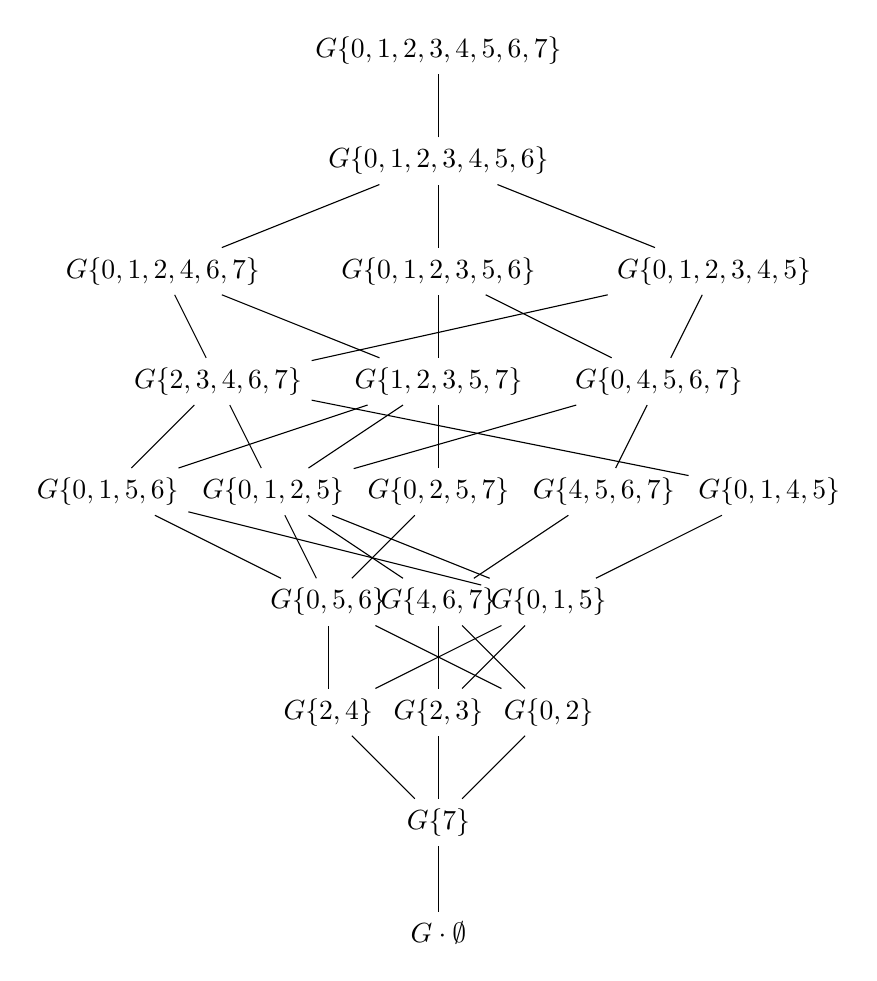
\begin{tikzpicture}[scale=.7]
  \node (0) at (0,-2) {$G\cdot\emptyset$};
  
  \node (1) at (0,0) {$G\{7\}$};
  
  \node (2) at (-2,2) {$G\{2,4\}$};
  \node (3) at (0,2) {$G\{2,3\}$};
  \node (4) at (2,2) {$G\{0,2\}$};
  
  \node (5) at (-2,4) {$G\{0,5,6\}$};
  \node (6) at (0,4) {$G\{4,6,7\}$};
  \node (7) at (2,4) {$G\{0,1,5\}$};
  
  \node (8) at (-6,6) {$G\{0,1,5,6\}$};
  \node (9) at (-3,6) {$G\{0,1,2,5\}$};
  \node (10) at (0,6) {$G\{0,2,5,7\}$};
  \node (11) at (3,6) {$G\{4,5,6,7\}$};
  \node (12) at (6,6) {$G\{0,1,4,5\}$};
  
  \node (13) at (-4,8) {$G\{2,3,4,6,7\}$};
  \node (14) at (0,8) {$G\{1,2,3,5,7\}$};
  \node (15) at (4,8) {$G\{0,4,5,6,7\}$};
  
  \node (16) at (-5,10) {$G\{0,1,2,4,6,7\}$};
  \node (17) at (0,10) {$G\{0,1,2,3,5,6\}$};
  \node (18) at (5,10) {$G\{0,1,2,3,4,5\}$};
  
  \node (19) at (0,12) {$G\{0,1,2,3,4,5,6\}$};
  
  \node (20) at (0,14) {$G\{0,1,2,3,4,5,6,7\}$};

  \draw (0) -- (1);
  
  \draw (1) -- (2);
  \draw (1) -- (3);
  \draw (1) -- (4);
  
  \draw (2) -- (5);
  \draw (2) -- (7);
  \draw (3) -- (6);
  \draw (3) -- (7);
  \draw (4) -- (5);
  \draw (4) -- (6);
  \draw (5) -- (8);
  \draw (5) -- (9);
  \draw (5) -- (10);
  \draw (6) -- (9);
  \draw (6) -- (11);
  \draw (7) -- (8);
  \draw (7) -- (9);
  \draw (7) -- (12);
  \draw (8) -- (13);
  \draw (8) -- (14);
  \draw (9) -- (13);
  \draw (9) -- (14);
  \draw (9) -- (15);
  \draw (10) -- (14);
  \draw (11) -- (15);
  \draw (12) -- (13);
  \draw (13) -- (16);
  \draw (13) -- (18);
  \draw (14) -- (16);
  \draw (14) -- (17);
  \draw (15) -- (17);
  \draw (15) -- (18);
  \draw (16) -- (19);
  \draw (17) -- (19);
  \draw (18) -- (19);
  \draw (19) -- (20);
\end{tikzpicture}
\caption{}
\end{figure}

\ssec{A Failed Attempt for Showing $\mathcal E(B_n/G)$ is unimodal}

In this section, we describe one path we were pursuing in order to show $\mathcal E(B_n/G)$ is unimodal. We were attempting to do this by trying to show there were injective order raising maps $U_i:\mathcal E(B_n/G)_i \rightarrow \mathcal E(B_n/G)_{i+1}.$

We shall now define several maps, so that we can draw a certain commuting diagram in Remark ~\ref{failed_commuting_diagram}


\begin{note}
Let $U_i:P_i \rightarrow P_{i+1}$ be the raising operator for the poset $P.$ Then, we obtain an induced map
\begin{align*}
	U_i \otimes U_{i+1}:P_i\otimes P_{i+1} \rightarrow P_{i+1} \otimes P_{i+1},(x,y) \mapsto U(x) \otimes U(y).
\end{align*}

We also have the natural inclusions
\begin{align*}
	k_i:\mathcal E(P)_i &\rightarrow P_i \otimes P_{i+1},\\
	(x, y) &\mapsto (x, y)\\
	k_i^{G\times G}:\mathcal E(P/G)_i &\rightarrow (P/G)_i \otimes (P/G)_{i+1},\\
	(Gx, Gy) &\mapsto (Gx, Gy),
\end{align*}
where we have $x \lessdot y$ and $Gx \lessdot Gy.$ The maps above are defined on a basis, and are extended by linearity.

Next, we define the map
\begin{align*}
	j_i:\mathcal (P/G)_i \otimes (P/G)_{i+1} & \rightarrow P_i \otimes P_{i+1},\\
	(Gx, Gy) &\mapsto \left(\frac{1}{|G|}\sum_{g \in G}^{} gx, \frac{1}{|G|}\sum_{h\in G}^{}hy).\right)
\end{align*}
where $x$ is an arbitrary representative of $Gx$ and $y$ is an arbitrary representative of $Gy$

Then, define the map
\begin{align*}
	p_i: P_i \otimes P_{i+1} &\rightarrow \mathcal (P/G)_i \otimes (P/G)_{i+1},\\
	(x, y) &\mapsto (Gx, Gy).
\end{align*}

Further, define the map 
\begin{align*}
	(U_i \otimes U_{i+1})^{G\times G}:P_i\otimes P_{i+1} &\rightarrow P_{i+1} \otimes P_{i+1},\\
	(Gx, Gy) &\mapsto p_{i+1}\circ(U_i \otimes U_{i+1})\circ j_i(Gx, Gy).
\end{align*}

We also have the projections inclusions
\begin{align*}
	\pi_i:P_i \otimes P_{i+1} & \rightarrow \mathcal E(P)_{i},\\
	(x, y) &\mapsto  \begin{cases}
	(x, y), &\text{ if }x\lessdot y\\
	0 &\text { otherwise}
\end{cases}\\
	\pi_i^{G\times G}: (P/G)_i \otimes (P/G)_{i+1} &\rightarrow\mathcal E(P/G)_i,\\
	(Gx, Gy) &\mapsto \begin{cases}
	(Gx, Gy), &\text{ if }Gx\lessdot Gy\\
	0 &\text { otherwise}
\end{cases},
\end{align*}
where we have $x \lessdot y$ and $Gx \lessdot Gy.$ The maps above are defined on a basis, and are extended by linearity.

Finally, denote
\begin{align*}
	\mathcal E(U)_i:\mathcal E(P)_i &\rightarrow \mathcal E(P)_{i+1}\\
	(x, y) &\mapsto k_i \circ (U \otimes U) \circ \pi_{i+1}(x, y)\\
\mathcal E(U)^{G\times G}_i:\mathcal E(P/G)_i & \rightarrow \mathcal E(P/G)_{i+1}\\
	(Gx, Gy) &\mapsto k^{G\times G}_i \circ (U \otimes U)^{G\times G} \circ \pi^{G\times G}_{i+1}(Gx, Gy)
\end{align*}
where it is defined above on a basis and we extend to the whole space by linearity.
\end{note}

\begin{rem}
\label{failed_commuting_diagram}
For $i < \frac{n}{2}$ we obtain the following (almost commuting, but $j_{i+1}\circ p_{i+1} \neq \id.$) diagram

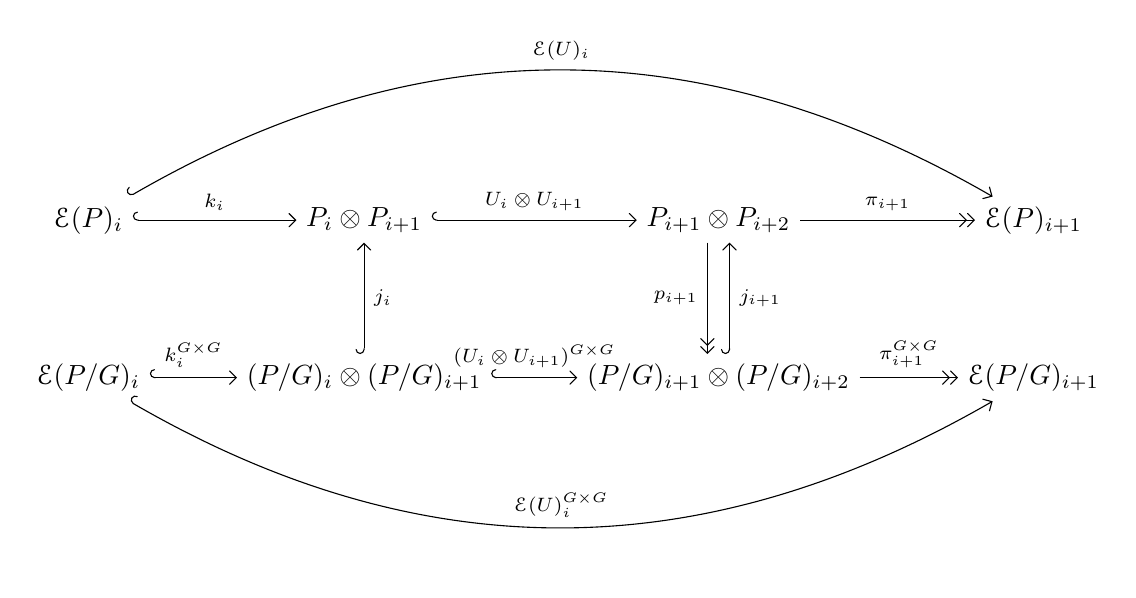
\begin{tikzpicture}[baseline=(current  bounding  box.center)]
\node (a) at (0,0) {$\mathcal E(P)_i$};
\node (b) at (3.5,0) {$P_i \otimes P_{i+1}$};
\node (c) at (8,0) {$P_{i+1} \otimes P_{i+2} $};
\node (d) at (12,0) {$\mathcal E(P)_{i+1}$};
\node (e) at (0,-2) {$\mathcal E(P/G)_i$};
\node (f) at (3.5,-2) {$(P/G)_i \otimes (P/G)_{i+1}$};
\node (g) at (8,-2) {$(P/G)_{i+1} \otimes (P/G)_{i+2} $};
\node (h) at (12,-2) {$\mathcal E(P/G)_{i+1}$};
\path[right hook->,font=\scriptsize,>=angle 90] ([xshift= 4pt]g.north) edge node[right] {$j_{i+1}$} ([xshift= 4pt]c.south)
(a) edge node[above]{$k_i$} (b)
(b) edge node[above]{$U_i\otimes U_{i+1}$} (c)
(e) edge node[above]{$k_i^{G\times G}$}(f)
(f) edge node[above] {$(U_i \otimes U_{i+1})^{G\times G}$} (g)
(f) edge node[right] {$j_{i}$} (b)
(a) edge [bend left] node[above] {$\mathcal E(U)_i$} (d)
(e) edge [bend right] node[above] {$\mathcal E(U)^{G\times G}_i$} (h)
;
\path[->>,font=\scriptsize,>=angle 90]
([xshift= -4pt]c.south) edge node[left] {$p_{i+1}$} ([xshift= -4pt]g.north)
(c) edge node[above] {$\pi_{i+1}$}(d)
(g) edge node[above] {$\pi_{i+1}^{G\times G}$} (h)
;
\end{tikzpicture}


Unfortunately, in general, with the above definitions of the maps, 
$$\ker \left(\pi^{G\times G}_{i+1}\circ p_{i+1}\right) \cap \im((U\otimes U)\circ j_i\circ k^{G\times G}_i)
\not\subset \ker \pi_{i+1} \cap \im((U\otimes U)\circ j_i\circ k^{G\times G}_i).$$
However, if we did have 
$$\ker \left(\pi^{G\times G}_{i+1}\circ p_{i+1}\right) \cap \im((U\otimes U)\circ j_i\circ k^{G\times G}_i)
\subset \ker \pi_{i+1} \cap \im((U\otimes U)\circ j_i\circ k^{G\times G}_i),$$
using the fact that $\mathcal E(U)_i,U_i,U_{i+1}$ are all injective, a fairly simple diagram chase would reveal $\mathcal E(U)_i^{G\times G}$ is injective. This, in turn, would imply $\mathcal E(B_n/G)_i$ is symmetric, unimodal, and Sperner.
We have tried several variations on these exact maps, but were never quite able to obtain the desired $\ker \left(\pi^{G\times G}_{i+1}\circ p_{i+1}\right) \cap \im((U\otimes U)\circ j_i\circ k^{G\times G}_i)\subset \ker \pi_{i+1} \cap \im((U\otimes U)\circ j_i\circ k^{G\times G}_i).$
\end{rem}

\ssec{Further Questions}

\sssec{Category Theoretic Properties}

First, it is worth noting that the functor $\mathcal E:\mathcal P \rightarrow \mathcal P$ is neither essentially surjective nor fully faithful. Let $P$ be the poset with points $a,b,c,d$ and relations $a \lessdot c, b \lessdot c, a \lessdot d.$ It is easy to see there is no poset $A$ with $\mathcal E(A) = P.$ This shows $\mathcal E$ is not essentially surjective. Next, let $Q$ be the poset whose elements are $e,f,g$ with $e \lessdot f, e \lessdot g,$ and let $R$ be the poset whose elements are $h,i,j,k$ with $h \lessdot i, j \lessdot k.$ It is clear that $\mathcal E(Q) \cong \mathcal E(R)$ are both a disjoint union of two points, but $Q \not \cong R.$ So, $\mathcal E$ is also not fully faithful.

However, there are many aspects of the functor $\mathcal E,$ and indeed $\mathcal E^{\vec r}$ which are still unexplored. First, note that it is worth noting that $\mathcal E$ also determines a endofunctor on the category of (ungraded) posets, which we shall now notate $\mathcal Q,$ as well as an endofunctor on the category of graded posets $\mathcal P.$ In general, the points of a poset $P$ can be identified with the set $Hom_{\mathcal Q}(B_0,P),$ and the edges of $P$ can be identified with the set $Hom_{\mathcal Q}(B_1,P).$ It is simple to see additionally that the points of $\mathcal E(P)$ are $Hom_{\mathcal Q}(B_0,\mathcal E(P)) \cong Hom_{\mathcal Q}(B_1,P).$ Additionally, the edges of $\mathcal E(P)$ are $Hom_{\mathcal Q}(B_1,\mathcal E(P)) \cong Hom_{\mathcal Q}(B_2,P).$ These relations may be a reasonable alternate way to think of the functor of points, and are further suggestive of the existence of an adjoint functor.

\begin{question}
Does the functor $\mathcal E$ have a left or right adjoint?
\end{question}

\sssec{Unitary Peck Generalizations}

Additionally, there are several posets which we would like to be unitary  
Peck, as this would allow us to apply much of the theory developed in this paper. They would also make several of the generalizations of $\mathcal E$ potentially more interesting. Two posets we are particularly interested in are $\mathcal E^{\vec r}(B_n)$ and its q-analog, $\mathcal E^{\vec r}(B_n(q)).$

\begin{question}
Is $\mathcal E^{\vec r}(B_n)$ unitary Peck?
\end{question}

As mentioned in the introduction, a natural extension of Conjecture ~\ref{conj:F_of_BnG_Peck} would be an analogous result for q-analogs. We suspect that a proof similar to that of Corollary ~\ref{cor:unitary_peck_edge_bn} may also prove Question ~\ref{question:unitary_peck_q_edge}.

\begin{question}
\label{question:unitary_peck_q_edge}
Is $\mathcal E(B_n(q))$ unitary peck? What about $\mathcal E^{\vec r}(B_n(q))?$
\end{question}

\sssec{A $q$-analog of Conjecture ~\ref{conj:F_of_BnG_Peck}}

In particular, if the answer to the previous Question ~\ref{question:unitary_peck_q_edge} is affirmative, it would immediately hold that $\mathcal E(B_n(q))/G$ is Peck, and if $G$ is CCT then $\mathcal E(B_n(q)/G)$ is Peck. Hence, we pose the following question: 

\begin{question}
For $G$ a group with a CCT action on $B_n(q)$ is $\mathcal E(B_n(q)/G)$ Peck?
\end{question}

Even more generally, we wonder if the q-analog of Conjecture ~\ref{conj:F_of_BnG_Peck} holds.

\begin{question}
For $G$ a group acting on $B_n(q)$, is $\mathcal E(B_n(q)/G)$ Peck? If not, is $\mathcal E(B_n(q)/G)$ rank unimodal?
\end{question}

\sssec{Additional CCT Actions}

We also found several additional interesting examples of CCT actions, and we are curious whether they generalize. Once such action is the linear automorphism of the $n$-cube. Using computers, we found that for $n \leq 3,$ the linear automorphisms of the $n$-cube is CCT. We wonder if this generalizes.

\begin{question}
Does the group of linear automorphism of an $n$-cube in $\BR^n$, whose vertices lie at $(\pm 1, \ldots, \pm 1)$ induce a common cover transitive action on $\BR^n$?
\end{question}

Also, we found using computers that the group of invertible linear maps on $\BF_2^3$ acting on the the seven nonzero points of $\BF_2^3$ induce an action on $B_7$ which is CCT. We wonder if this generalizes to other groups of invertible linear maps on finite fields.

\begin{question}
Is the action of $GL_n(\BF_q)$ on $B_{q^n-1}$ (induced by the action of $GL_n(\BF_q)$ on $(\BF_q^n)^*$) CCT? What about the action of $PGL_n(\BF_q)$ on $B_{q^n-1}?$ If not, what about the action of $PGL_n(\BF_2)$ on $B_{2^n-1}?$ 
\end{question}

\section*{Acknowledgements}
This research was carried out in the 2014 combinatorics REU program at the University of Minnesota, Twin Cities, and was supported by RTG grant NSF/DMS-1148634.
The authors would like to thank their mentor Victor Reiner for his consistent help and guidance throughout the project and their TA Elise DelMas for her helpful feedback on the paper. They would also like to thank Ka Yu Tam for helpful comments.  In addition, they thank the math department of University of Minnesota, Twin Cities, for its hospitality and Gregg Musiker for organizing the program.

\bibliography{References}
\bibliographystyle{alpha}


\end{document}
